\documentclass[11pt,a4paper]{report}
\usepackage[T1]{fontenc}
\usepackage[utf8]{inputenc}
\usepackage[margin=2cm]{geometry}
\usepackage{amsmath,amssymb,booktabs,longtable,array,xcolor,colortbl}
\usepackage{tikz,pgfplots}
\pgfplotsset{compat=1.18}
\usepackage[breaklinks=true,colorlinks=true,linkcolor=blue!45!black,urlcolor=blue!55!black]{hyperref}
\usepackage{xurl}
\definecolor{navy}{HTML}{174B65}
\definecolor{muted}{HTML}{8DA1AC}
\setlength{\parindent}{0pt}
\setlength{\parskip}{6pt}
\setcounter{tocdepth}{1}
\setcounter{secnumdepth}{1}
\makeatletter
\renewcommand{\l@section}{\@dottedtocline{1}{1.5em}{4em}}
\renewcommand{\l@figure}{\@dottedtocline{1}{1.5em}{4em}}
\renewcommand{\l@table}{\@dottedtocline{1}{1.5em}{4em}}
\makeatother
\emergencystretch=3em
\Urlmuskip=0mu plus 2mu\relax
\hypersetup{pdftitle={Caste Ties and Firm Growth in India's Mining Industry},pdfauthor={nakshatra0904}}
\begin{document}
\hypersetup{pageanchor=false}
\begin{titlepage}
\centering\vspace*{2cm}
{\Huge\bfseries Caste Ties and Firm Growth\par}
\vspace{0.5cm}{\LARGE India's Mining Industry\par}
\vspace{1cm}{\Large Public-data evidence, source inventory,\par fieldwork design and causal identification\par}
\vspace{1.5cm}{\large Detailed research report\par nakshatra0904\par 12 October 2026\par}
\vfill
\begin{minipage}{0.88\textwidth}
\textbf{Evidence boundary.} I analyzed historical aggregate data from the Sixth Economic Census and Census 2011, fitted nine regional establishment specifications and four controlled worker-duration models, and prepared nineteen figures and a 65-entry source inventory. I did not observe caste ties or longitudinal firm growth and have not estimated a causal caste-network effect. Prospective designs and trial-power calculations are explicitly identified as proposals.
\end{minipage}
\vspace{1cm}
\end{titlepage}
\pagenumbering{roman}
\hypersetup{pageanchor=true}
\chapter*{Abstract}\addcontentsline{toc}{chapter}{Abstract}
I extracted mining and quarrying tables containing 85,176 establishments and 557,474 workers. Within the proprietary subset, workers per establishment are 2.63 for SC owners, 3.68 for ST owners, 3.77 for OBC owners and 5.62 for the residual Others category. These aggregate ratios establish a historical difference in establishment scale. They do not identify a network mechanism, an individual-firm size distribution or growth. A demographic merge supports regressions for 35 historical state/UT regions and 35 Maharashtra districts. Adjusted log-size associations with SC and ST population shares have wide HC3 intervals. One unadjusted state-density coefficient has $p=0.036$, but its Benjamini--Hochberg value is $0.651$ across the specified 18-coefficient family. A detailed prospective design combines consent-based relationship measurement, repeated firm outcomes, administrative linkage and a randomized business-introduction intervention. The added Census worker baseline contains 2,105,736 workers, 20.87 percent SC and 17.32 percent ST. Within state-division-sex-residence strata, employment-weighted SC and ST marginal-duration contrasts versus the residual group are +1.49 and +5.08 percentage points; these are descriptive adjusted associations. Local Rajasthan studies report job-entry routes, caste composition and working conditions; Coal India administrative snapshots add employee and vacancy information. I retained all observed-data tables, all nineteen figures, source access classifications and fieldwork modules in this reproducible package.
\tableofcontents\listoffigures\listoftables\clearpage
\pagenumbering{arabic}

\chapter{Research question and what this report establishes}
I developed a dissertation research programme on caste relationships and enterprise growth in India's mining economy, and completed the empirical analyses supported by the public data I acquired. The central finding is a substantial descriptive difference in the employment scale of proprietary mining establishments across owners' broad social groups. The central identification finding is equally important: the available tabulations do not observe business relationships or repeated outcomes for the same firm. They therefore cannot identify the causal effect of caste ties on growth. The completed regressions describe geographic associations; the fieldwork and causal designs specify how to answer the original question credibly.

I used three source documents for my original establishment analysis: the government-authored All India Report of the Sixth Economic Census, Maharashtra's Sixth Economic Census report, and the Census of India 2011 Primary Census Abstract spreadsheet. I obtained the national report from an Ecensus mirror after official download attempts failed, and the Maharashtra report from NITI for States. I retained source files, acquisition routes, hashes, table locations, extracted data, transformations, statistical outputs and figures in my research package. These are historical data, principally 2011 and 2013-14, not a description of the mining economy in 2026. \hyperlink{S02}{[S02]} \hyperlink{S07}{[S07]} \hyperlink{S09}{[S09]}

There are 85,176 mining and quarrying establishments and 557,474 workers in the extracted national tables. The proprietary subset contains 73,170 establishments and 319,425 workers. Among that subset, workers per establishment are 2.63 for SC owners, 3.68 for ST owners, 3.77 for OBC owners and 5.62 for the residual Others category. These are ratios of employment totals to establishment totals, not medians of individual firms. The SC ratio is about 46.9 percent of the Others ratio. That difference motivates research on resources, market access and exclusion, but does not by itself establish any one mechanism.

I fitted nine regional OLS specifications. The national demographic merge contains 35 historical state/\allowbreak{}UT regions after pooling residual Andhra Pradesh and Telangana to match the 2011 undivided Andhra Pradesh geography. Log-size models have 33 observations because Delhi and Lakshadweep have no mining establishments in the extracted table. The Maharashtra replication contains 35 historical districts. Adjusted log-size associations with regional SC and ST population shares are imprecise. One SC coefficient in the state density model has an unadjusted p-value of 0.036, but the Benjamini-Hochberg adjusted value is 0.651 for the specified family of 18 social-composition coefficients. No causal conclusion follows from it.

I propose building a consent-based owner and business-relationship panel, linked where authorized to mine, lease, company and procurement identifiers. Fieldwork should cover operators and contractors separately, include both registered and less visible businesses, and follow surviving firms, exits and new entrants. A randomized introduction or procurement-brokerage intervention is the most defensible prospective route to a causal estimate of access to business relationships. Observational policy designs remain useful, but must establish a credible comparison group and cannot simply label a policy coefficient a caste-network effect.

I extended the analysis with official Census B18, B18SC and B18ST counts, two Coal India employee snapshots, selected recruitment disclosures and published Rajasthan worker evidence. The worker baseline contains 2,105,736 people in NIC divisions 05-09. Four fitted aggregate duration models show how SC/\allowbreak{}ST differences change with sex, rural/\allowbreak{}urban residence, state and mining division controls. The expanded inventory has 65 entries, the report includes nineteen graphs, and the questionnaire now has 86 draft measures including 30 worker/\allowbreak{}job-entry items. The worker chapter specifies source-specific denominators and limitations. \hyperlink{S56}{[S56]} \hyperlink{S57}{[S57]} \hyperlink{S58}{[S58]} \hyperlink{S59}{[S59]} \hyperlink{S60}{[S60]} \hyperlink{S61}{[S61]} \hyperlink{S62}{[S62]}

\section{Evidence status}
I completed source discovery and classification; downloading the three actual inputs; extracting national state tables and 23 industry by four social-group cells; constructing state and district demographic joins; checking arithmetic; producing descriptive statistics, correlations, nine OLS models, HC3 intervals, influence diagnostics, leave-one-out ranges, multiple-testing corrections, aggregate industry fixed-effect contrasts, twelve establishment graphs and illustrative trial-power calculations; the worker extension adds seven graphs and four employment-weighted controlled comparisons.

I did not conduct interviews, invent respondents or access a proprietary firm panel. No actual caste-tie variable, firm sales-growth series, individual-firm survival history, randomized assignment, policy treatment panel, instrumental-variable first stage or valid regression-discontinuity running variable was acquired. Consequently, I have not estimated a causal effect of caste ties or regressed observed mining firm growth on observed caste ties. I developed a detailed research specification for those analyses once the required data exist.

I assembled an expanded source inventory containing 65 entries, including documents, databases, administrative systems and source families. It is deliberately broad, but cannot certify that every possible Indian record has been located. Entries distinguish downloaded inputs, verified public documentation, conditional or commercial access, candidate source families and primary data still to be collected. A portal's existence is not treated as proof that its transaction-level data are publicly downloadable.

\chapter{Conceptual framework}
\section{Caste identity and caste ties are different objects}
An owner's broad category is an attribute. A caste tie is a relationship with another person or organization that may transmit information, trust, credit, labour, referrals, political access or obligations. A person can share a broad category with another entrepreneur without sharing a jati or any actual relationship. Conversely, a business tie can cross jati, category, religion or locality. Administrative SC, ST, OBC and residual classifications must not be treated as four internally uniform social networks.

I propose distinguishing at least four measurements in my future fieldwork. First, record self-reported broad social category and optional self-described jati. Second, observe named or coded business contacts and the respondent's own account of whether a relationship is connected to shared community identity. Third, record what each contact actually did, when it occurred and whether money or business information changed hands. Fourth, measure the eligible opportunity set: nearby businesses, procurement buyers, lenders, labour brokers and associations with which contact could plausibly have occurred.

Scheduled Tribe identity also deserves a distinct analytical treatment. Adivasi social organization, community claims, land access, displacement and the institutional circumstances of mining are not adequately represented by assuming they are identical to caste-based entrepreneur networks. SC and ST results should be presented separately before any pooled disadvantaged-group analysis. The EC residual Others category is a coding residual; it is not a validated indicator of upper-caste identity or dominance. \hyperlink{S01}{[S01]} \hyperlink{S13}{[S13]}

I will not infer individuals' caste from surnames, photographs, geography, directors' names or association labels. Identity and relationship information should come from voluntary self-report or an explicitly authorized administrative classification, with a separate unknown or declined-response code. This preserves construct validity and avoids turning uncertain social classification into a hidden measurement error.

\section{Mechanisms and competing hypotheses}
H1 is an information mechanism: community contacts reduce the cost of learning about leases, tenders, buyers, equipment and credit. H2 is an enforcement mechanism: repeated social interaction permits trade credit and informal insurance where legal collection is costly. H3 concerns labour recruitment and monitoring: referrals can ease hiring, but may also segment jobs and exclude outsiders. H4 concerns access to gatekeepers: connected firms may navigate administrative requirements or secure introductions more quickly. These hypotheses require process measures, not merely a coefficient on owner category.

H5 is a constraint mechanism. Dense within-community networks can lock firms into a narrow buyer pool, impose transfers or obligations, and discourage relationships outside a familiar market. H6 is an exclusion mechanism: established networks may screen out entrepreneurs from historically disadvantaged groups even when those entrepreneurs have comparable productive capabilities. The effect of ties can therefore vary by type of contact, social location, mineral, scale and institutional setting. A single positive or negative average coefficient would conceal that heterogeneity.

Resources and selection produce competing explanations. Wealthier households may both enter capital-intensive mining and sustain influential contacts. Larger firms may attract buyers and lenders, creating ties as a consequence of success. Migration may alter both network composition and business opportunities. Technology, concession size, mineral quality, inherited land, local demand and formal-company organization can generate size differences even if relationships have no causal effect. The report treats these alternatives as hypotheses to discriminate, not as explanations already demonstrated.

The literature offers motivation rather than a transferable mining estimate. Iyer, Khanna and Varshney's work establishes the usefulness of Economic Census ownership information for studying entrepreneurship and social hierarchy. Munshi and Rosenzweig examine how traditional networks can influence choices and mobility in a different setting. Neither study licenses extrapolating a causal coefficient to Indian mining firms. The research contribution here would be direct relationship measurement in a sector with strong licensing, geology and buyer concentration, followed by longitudinal or experimental identification.

\section{Outcomes and estimands}
The preferred primary outcome is employment growth over a pre-specified interval, with real sales growth and survival as separate outcome families. A secondary outcome is production growth in mineral-specific physical units. Employment should separate owner work, unpaid family work, directly hired labour and contract labour. Sales should separate production sales, trading revenue and inter-company transactions. A firm with several mines requires both establishment-level and legal-entity-level accounts.

For continuing businesses with positive employment at both dates, annualized log employment growth is defined as follows. It should be supplemented by levels and by a symmetric growth measure that handles entry and exit, since conditioning only on survivors selects on an outcome affected by relationships.

\[
g_i^{E}=\frac{\log E_{i,t_1}-\log E_{i,t_0}}{t_1-t_0},\qquad
g_i^{DHS}=\frac{2(E_{i,t_1}-E_{i,t_0})}{E_{i,t_1}+E_{i,t_0}}.
\]
For a prospectively randomized brokerage offer, the primary estimand is the intention-to-treat effect of being offered the programme among eligible baseline firms. A treatment-on-the-treated interpretation for actual relationship formation needs additional assumptions. It is inappropriate to describe the effect of an offer containing training, information and introductions as the pure effect of caste ties. Those components must be measured and, where feasible, separated by design.

\[
\operatorname{ITT}=\mathbb{E}[Y_i(1)-Y_i(0)],\qquad
Y_i(z)=\text{outcome under assignment }z.
\]
For the observational panel, the target must be stated as an association unless a defensible identification argument is supplied. A one-standard-deviation increase in a pre-specified relationship index, a new buyer introduction and a change in within-jati tie share are different exposures and estimands. The dissertation should not switch among them after inspecting which specification is significant.

\chapter{Mining sector scope and the empirical population}
\section{Operators and the mining supply chain}
The core operator universe uses the relevant mining and quarrying classification. NIC 2008 Section B covers divisions 05 through 09, including coal and lignite, petroleum and natural gas, metal ores, other mining and quarrying, and support activities. The Sixth EC broad activity code 05 is a broad mining category; it is not NIC division 05, which specifically denotes coal and lignite. Confusing those two code systems would create a serious sample error. \hyperlink{S01}{[S01]} \hyperlink{S02}{[S02]}

Mining-dependent suppliers can belong to transport, machinery repair, construction, trading, professional services or other classifications. A supplier should be included on the basis of a documented mining revenue share or verified mining contracts, not on its industry code alone. A practical threshold is to pre-specify a mining sales-exposure measure and retain the continuous share for robustness. Operator estimates and supplier estimates should be reported separately even when both populations are sampled in the same district.

Major-mineral mines, small stone quarries, sand operations, coal enterprises and hydrocarbon operators face different reporting and concession regimes. The all-India public-data analysis is broad; the prospective fieldwork should concentrate on populations in which owner relationships can be measured reliably and enough independent businesses exist. Large public enterprises can serve as buyers and institutional context, but their own output cannot be attributed to an entrepreneur's caste network.

\section{Geographic priorities}
An initial core could combine Rajasthan's stone and quarrying businesses, Odisha's mineral and contractor ecosystem, and Maharashtra's quarrying and contractor population. The inclusion of Maharashtra is supported by an actually acquired district dataset, which permits frame checks and a transparent replication. Odisha has a verified public lessee register and an administrative system with stable codes. Rajasthan offers a potentially useful small-operator setting, but its current frame needs to be acquired and checked before district selection. \hyperlink{S07}{[S07]} \hyperlink{S33}{[S33]} \hyperlink{S34}{[S34]} \hyperlink{S35}{[S35]}

The final cluster list should be chosen after a short listing pilot rather than by declaring well-known mining districts representative. Stratify within states by mineral, formal operator versus contractor, approximate scale, rurality and lease or contract status. Include commercially active locations and areas with small or intermittent operations. Oversample groups with small entrepreneur counts, while retaining probabilities and survey weights so the target population remains explicit.

Geography must be historical when historical data are used. The national merge pools EC residual Andhra Pradesh and Telangana into the 2011 state of Andhra Pradesh. The Maharashtra merge uses 35 districts in their historical configuration, including Thane before Palghar's later separation and the older names in the source. Present-day district maps should not be applied to these counts without a documented crosswalk. There is no spatial regression or geocoded mine map in the completed analysis.

\chapter{Data discovery and acquisition strategy}
\section{Four layers of evidence}
Layer 1 is the establishment frame: Economic Censuses, state directories, lease registers, Udyam and a new area listing. Layer 2 is outcomes: authorized mine returns, company accounts, production and dispatch records, procurement contracts and repeated field measurements. Layer 3 is relationships: a consented owner and alter module, association participation and dated introductions. Layer 4 is context: geology, mineral prices, transport access, population composition and institutional events.

No single identified source provides all four layers. Economic Census data are particularly useful for broad coverage and owner category but weak for direct relationships and firm-level growth. Company panels provide financial trajectories but exclude many small businesses and do not supply validated owner caste. Administrative mining records may provide physical outcomes and concession events but require access verification and still need a relationship module. IHDS offers household social-capital questions and longitudinal household information, with mining sample size and business attribution still to be checked. \hyperlink{S01}{[S01]} \hyperlink{S12}{[S12]} \hyperlink{S20}{[S20]} \hyperlink{S37}{[S37]} \hyperlink{S39}{[S39]}

ASUSE and the related unincorporated manufacturing, trade and service sources need a coverage check before use. The checked official coverage excludes mining Section B. They may be valuable for eligible ancillary enterprises, but treating them as a mining-operator dataset would misstate the population. ASI likewise requires an explicit factory and industry eligibility check; mineral processing and manufacturing are not automatically the same population as mine operators. \hyperlink{S15}{[S15]} \hyperlink{S16}{[S16]}

\section{Acquiring usable records}
First request original EC5 and EC6 microdata through the official registered access route, schedules, record layouts and code lists. Obtain social group by mining by district tabulations if direct unit access is delayed. Retrieve the official distribution when possible to verify the mirrored national report byte-for-byte or reconcile content differences. Do not mix provisional and final census totals. The official FAQ checked during this work describes seventh-census finalization; an unverified final seventh-census file is not included. \hyperlink{S03}{[S03]} \hyperlink{S05}{[S05]}

Second request a deidentified mine-month or mine-year panel from IBM and the selected state departments, including mine code, lease holder, mineral, physical output, employment, dispatch, operational status, filing status and revisions. Ask for unsuccessful and non-operating records as well as operating mines. A returns system can omit precisely the businesses most likely to exit or remain informal. Administrative non-filing must not be silently recoded as zero production. \hyperlink{S20}{[S20]} \hyperlink{S21}{[S21]} \hyperlink{S34}{[S34]}

Third seek the university's Prowess licence or authorized MCA research access. Define entity identifiers and preserve standalone and consolidated financial statements. Add procurement bidder and award records for a clearly scoped set of buyers and services. Losing bidders and eligibility failures are particularly valuable: a winners-only dataset cannot estimate the probability of obtaining a contract. Obtain the relevant portal terms before downloading or redistributing restricted extracts. \hyperlink{S38}{[S38]} \hyperlink{S39}{[S39]} \hyperlink{S45}{[S45]}

Fourth undertake field listing and an owner panel. Record permission for each linkage, maintain contact information outside the analytical files, and use a stable pseudonymous firm identifier. Mine codes, legal firms and operating establishments form a many-to-many system. The linkage table must preserve ownership transfers, separate subsidiaries and multiple mines, rather than collapsing them into a deceptively simple one-row-per-company file.

\section{Access status and search limits}
The archive includes an acquisition log with successful and failed attempts. The official national-report landing and some older MoSPI download routes did not yield a usable report during my acquisition attempts, while a government-authored mirror did. EC microdata metadata were discoverable, but the requested downloadable unit records were not acquired. Original microdata have not been replaced with invented establishment observations or surname-derived owner labels.

The 65-entry appendix records source-specific access and analytical roles. Families such as GST, payroll, bank credit, GeM, state-board consents, other state mining departments, exporter records and association lists remain conditional research leads. Their presence in the appendix is not a claim of access or an assessment of every file's schema. I have not sent institutional data requests or opened accounts to obtain restricted research records.

\chapter{Construction of the completed analytical data}
\section{Extraction and source traceability}
The national report contributes Table 2.5 on mining establishments at PDF page 145, printed page 135, and Table 4.5 on mining employment at PDF page 169, printed page 159. Table 12 at PDF page 195, printed page 185, and Table 15 at PDF page 198, printed page 188, provide industry by owner-group establishment and employment totals. The Maharashtra report contributes Table 2.5 at PDF page 123, printed page 117, and Table 4.5 at PDF page 147, printed page 141. Page references are one-based.

I extracted the trailing numerical columns for each geography and checked every row against own-account plus hired-establishment totals, rural plus urban totals and combined counts. The extracted national totals reconcile to 85,176 establishments and 557,474 workers. The Maharashtra totals reconcile to 6,229 establishments and 29,527 workers and match the national Maharashtra row. The four mining owner-group counts reconcile to 73,170 proprietary establishments and 319,425 workers.

The numerical columns labelled employment in establishments with at least one hired worker include all persons working in those establishments. They are not counts of hired workers alone. Similarly, an own-account establishment has no hired worker under the census definition but may involve several household members. Misreading these columns would distort both employment shares and average size.

There are 92 aggregate industry-group observations, consisting of 23 broad industries crossed with four owner groups. These are not 92 sampled firms and are certainly not 52 million independent microdata rows. I therefore computed the industry contrasts as ratios of published counts and reported descriptive point estimates without manufacturing firm-level standard errors.

\section{Demographic joins and transformations}
The PCA input supplies total population, SC population, ST population, urban population and literate population at state and district levels. I joined state codes to historical geographic units after correcting Andhra Pradesh, and checked Maharashtra district names against both the source names and the historical district codes. The completed merge retains all 35 state/\allowbreak{}UT regions and all 35 Maharashtra districts; no unmatched geography is silently dropped.

\[
\overline E_r=\frac{W_r}{N_r},\qquad
d_r=100000\frac{N_r}{P_r},\qquad
h_r=100\frac{N_r^{H}}{N_r}.
\]
Here W is workers, N is establishments, P is the 2011 population and NH is the count of establishments with at least one hired worker. The population reference date differs from the establishment enumeration period. Density is a contextual historical measure with that timing limitation. SC and ST shares equal their population counts divided by total population, multiplied by 100. Literacy equals the literate population divided by population aged seven and above, not total population.

Size and hired shares are undefined when establishments are zero. They remain missing for Delhi and Lakshadweep; they are not filled with zero. Density includes the zeros. The density regression uses log of one plus establishments per 100,000 residents, making that dependent variable explicitly different from log density. The 50-establishment restriction is a sensitivity analysis intended to reduce instability in small district denominators, not a rule for deleting genuine large mines.

\section{Quality and measurement limitations}
Arithmetic reconciliation validates extraction, not census completeness. Under-enumeration, industry miscoding, intermittent activity and ownership classification can remain. The EC does not supply a verified longitudinal business identity in these tabulations. The national ownership categories are reported for proprietary establishments; incorporated operators, partnerships and public enterprises do not inherit a caste label from a table about proprietors.

The mineral composition of a region is not observed in the completed regressions. Major metal mines, smaller stone units and support activities can have very different labour intensity. This missing composition is a plausible explanation of geographic variation. Local demographics and infrastructure may also influence selection into mining. The report does not claim that basic literacy and urbanization controls remove these confounders.

The package preserves raw numerical counts and full-precision transformations. Rounded published percentages are retained for checking, while reported shares are recomputed from counts. The distinction matters because rounded percentages may sum to 100.1 or 99.9 without any extraction error. Unknown categories, non-applicable ownership and true zero establishments should be kept conceptually separate.

\chapter{Descriptive findings}
\section{Ownership and scale}
The national average is 6.54 workers per mining establishment when employment and establishments are summed before division. About 73.74 percent of establishments are rural. About 52.03 percent have at least one hired worker, and those establishments account for 88.84 percent of workers in the mining table. Proprietary businesses comprise 85.90 percent of establishments but 57.30 percent of mining employment. This indicates that the establishment frame is dominated numerically by proprietors while employment is more concentrated in larger and other organizational forms.

Within proprietary mining, SC owners account for 12.03 percent of establishments but 7.25 percent of workers. ST owners account for 8.87 percent and 7.47 percent respectively; OBC owners account for 38.93 percent and 33.60 percent. Others account for 40.18 percent of establishments and 51.68 percent of workers. Employment in a social-group row is employment at establishments owned by that group. It is not employment of workers from that group.

The SC mean is about 53.1 percent lower than the Others mean. The ST and OBC means are about 34.5 and 32.9 percent lower respectively. This is meaningful for describing business scale in this historical proprietary population. It cannot establish whether differences arise at entry, through subsequent expansion, through survival, through mineral specialization or through access to finance and contracts. Those explanations require different data and empirical tests.

Comparing owner shares with the whole population can provide a rough context, but it is not a properly adjusted entrepreneurship participation rate. The eligible-owner denominator depends on age, location, labour-market attachment, household resources and business opportunity. A national OBC participation ratio cannot be calculated from the acquired PCA because that source has no comparable general OBC population denominator. Broad Others categories also differ across datasets.

\section{Geography and heterogeneity}
After combining Andhra Pradesh and Telangana, the five largest state/\allowbreak{}UT regions account for 49.41 percent of establishments and 51.25 percent of workers. The establishment Herfindahl index is 0.0722 and the employment index is 0.0768 across those historical regions. These indices describe geographic concentration, not firm market concentration or buyer competition. They are affected by region size and aggregation.

The unweighted mean of the 33 non-empty regional size ratios is 9.18 workers, while their median is 6.48. These differ from the national 6.54 because the national ratio weights each regional mean by its establishment count. An average of regional ratios answers a different question from the ratio of national totals. The discrepancy is particularly large when small regions contain a few large operations.

Maharashtra has 6,229 mining establishments and 29,527 workers, for a pooled mean of 4.74 workers. Across districts the unweighted mean is 5.73 and the median is 3.15. Chandrapur's ratio is 58.5 workers per establishment, reflecting 5,148 workers across 88 establishments in the table. This is not a reason to classify the observation as an error: it is a reason to inspect sector composition and influence. The 23-district restriction with at least 50 establishments yields another explicit target population.

The report provides raw regional counts, denominator-based indicators, distribution summaries, rank figures, social-group shares, cross-industry ratios and the state correlation matrix. Histograms describe distributions of regional mean sizes. They do not describe the individual-firm employment distribution. Individual medians, firm-size percentiles, inequality within owner groups, and the fraction of SC mining firms above a given size cannot be recovered from the acquired aggregates.

\section{Cross-industry contrasts}
An aggregate descriptive model relates log of the group-specific industry mean size to industry indicators and group indicators. With equal weight per industry-group cell, the fitted SC contrast is -0.261 log points, approximately 23.0 percent smaller than Others. The OBC and ST contrasts are approximately 16.6 and 15.3 percent smaller. With establishment-count weights, the SC contrast is about 17.5 percent smaller and the OBC and ST contrasts about 13.5 and 13.4 percent smaller.

These results are summaries of published cell means across industries. Changing the weights changes the target summary, so the two estimates are not robustness proofs for a causal parameter. The particularly large raw mining SC contrast is useful for prioritizing a sector-specific investigation. It cannot show that a mining mechanism is statistically different from an individual-firm mechanism in other industries. No sampling p-values are presented for the cell models.

\chapter{Regression methods and completed results}
\section{Specifications}
The completed regional models use a baseline specification with SC and ST population shares, and an adjusted specification adding urban population share and literacy. All shares are scaled so a unit increase means ten percentage points. The source observations are regions, not individual owners. The dependent variables are log mean employment size, log of one plus establishment density, and the share of establishments with at least one hired worker. Each outcome has its own units.

\[
\log \overline E_r=\alpha+\beta_{SC}\frac{s_{SC,r}}{10}
+\beta_{ST}\frac{s_{ST,r}}{10}
+\gamma_U\frac{u_r}{10}+\gamma_L\frac{\ell_r}{10}+\varepsilon_r.
\]
S1 is the state log-size baseline. S2 adds the two controls. S3 repeats the adjusted size model among the 28 historical states excluding 2011 UTs. S4 uses transformed establishment density across all 35 regions, including zero-count regions. S5 uses the hired-establishment share in 33 non-empty regions. D1, D2 and D3 repeat adjusted size, density and hired-share models in the 35 Maharashtra districts. D4 restricts adjusted district size to the 23 districts with at least 50 establishments.

I used HC3 heteroskedasticity corrections and t-based intervals for the regional OLS models. The HC3 adjustment gives greater weight to the uncertainty introduced by high-leverage observations. These are model-based uncertainty summaries across a hypothetical population of comparable regions; the published census counts are not a random sample of these particular regions. Spatial dependence remains unaddressed because verified coordinates or a contemporaneous boundary adjacency file were not acquired. HC3 is not a correction for all spatial correlation.

\section{Main coefficients and interpretation}
In S2, the SC coefficient is 0.0306 with a 95 percent interval from -0.4932 to 0.5544; the ST coefficient is 0.0084 with an interval from -0.1421 to 0.1589. These associations are small at their point estimates but extremely imprecise. For example, the SC interval permits a substantial negative or positive relationship of local population composition with regional mean mining size. It does not permit a confident finding of no relationship.

In D1, the SC coefficient is -0.0406 with an interval from -0.6760 to 0.5948. The ST coefficient is 0.1273 with an interval from -0.2685 to 0.5230. The district data similarly do not identify a stable adjusted association. The ecological regressions should therefore be used as a description of context and a check against overconfident geographic narratives, not as an owner-level caste-effect analysis.

S4 yields an SC coefficient of -0.5284 on log of one plus establishment density, with an unadjusted p-value of 0.0362. A ten-percentage-point difference in SC population share corresponds to a fitted factor exp(-0.5284), about 0.59, for one plus density, conditional on the included controls. This cannot simply be reported as a 41 percent reduction in density itself, particularly near zero. The association may reflect geology, mineral composition, administrative coverage, region size or other omitted factors.

I defined an exploratory testing family of eighteen SC/\allowbreak{}ST coefficients across the nine regional models and calculated Holm and Benjamini-Hochberg adjustments, which I retained in the CSV. The S4 SC adjusted value is approximately 0.651; no coefficient meets a 5 percent threshold after the corrections. The models and sample restrictions were selected for feasibility and sensitivity analysis rather than chosen after screening for significance. This remains exploratory work, not a preregistered confirmatory study.

\section{Influence and robustness}
Cook's distances and leverage are retained for every observation in every OLS model. Leave-one-out coefficient ranges show how a fitted relationship changes when each region is removed in turn. The report also contrasts inclusion and exclusion of UTs and removes very small district denominators in D4. Such checks can reveal instability, but they do not cure omitted geology or replace direct network measurement.

When a large mine creates a high district average, deleting it would change the question from all mining establishments to a selected small-scale segment. The appropriate response is to collect mineral, organizational form and operating-scale information, then stratify or model those features. Winsorization should be a pre-specified sensitivity exercise, not a method of forcing a convenient coefficient. I did not winsorize the completed model data.

The raw regression table includes all intercepts and control coefficients, sample sizes, R-squared values, HC3 standard errors, raw p-values and confidence intervals. The source package also contains the influence file, the correlation matrix and full descriptive output. I emphasize social-composition coefficients in my main discussion because they address the research question, and I retain the other fitted terms in the complete results.

\chapter{Mining workers: caste composition, job entry and employment conditions}
\section{What the additional evidence contributes}
Worker composition is observable in several sources, even though caste-linked recruitment and firm growth remain incompletely observed. I added a national Census worker baseline, Coal India administrative employee snapshots, published recruitment flows and two Rajasthan stone-sector studies. They answer different questions. Census records industry-classified persons; Coal India records corporate employees; Rajasthan studies interview selected workers across extraction and processing. None supplies a linked national employer-worker network panel. I used actual published cells and retained their denominators, geographical coverage, dates and source locations. \hyperlink{S56}{[S56]} \hyperlink{S57}{[S57]} \hyperlink{S58}{[S58]} \hyperlink{S59}{[S59]} \hyperlink{S60}{[S60]} \hyperlink{S61}{[S61]} \hyperlink{S62}{[S62]}

The first distinction is between workers' own social identity and their employers' identity. EC6 employment classified by the proprietor's group does not reveal the group of the people employed. The B18 SC and ST tables directly classify workers by their own broad group. These series therefore substantially improve the labour-side description, but cannot be merged to EC6 to construct a worker-employer pairing. The second distinction is between a route into employment and the social identity of the person providing that route. A relative or colleague can provide a referral without sharing a caste; a same-category contact need not share a jati. Recruitment through relationships is evidence of relational hiring, rather than a direct measure of caste homophily.

\section{National Census extraction and population definitions}
I used three official Census 2011 Excel workbooks: B18 all persons, B18SC and B18ST. I selected NIC 2008 divisions 05, 06, 07, 08 and 09, with group code 000 and class code 0000. This avoids counting a division and then counting its constituent groups and classes again. The five divisions cover coal/\allowbreak{}lignite, petroleum/\allowbreak{}natural gas, metal ores, other mining/\allowbreak{}quarrying and mining-support services. Historical state codes 01-35 are retained; code 00 is the separate India total and never enters the regression. \hyperlink{S56}{[S56]} \hyperlink{S57}{[S57]} \hyperlink{S58}{[S58]}

The national total is 2,105,736 main plus marginal workers in the selected divisions. SC workers number 439,519, or 20.87 percent, and ST workers number 364,749, or 17.32 percent. The remaining 1,301,468 workers, or 61.81 percent, are derived by subtraction. That remainder contains OBC and other workers; it is not an upper-caste population. The source does not provide an OBC worker table. I did not manufacture a population-wide OBC denominator from the remainder.

Main workers worked for at least six months during the preceding reference year; marginal workers worked for less than six months. This is an annual-duration distinction. It does not classify permanent versus temporary contracts, regular versus contractor payroll, skilled versus unskilled employment, or insured versus uninsured workers. It also includes industry-classified workers beyond wage employees. Thus a marginal-worker share is a defensible duration outcome, while calling it the informal-employment rate would be incorrect. The official definitions are also available at \url{https://data.gov.in/catalog/main-workers-marginal-workers-non-workers-and-those-marginal-workers-non-workers} .

I checked every extracted numeric column for male plus female equalling persons and rural plus urban equalling total. SC and ST counts must not exceed the corresponding all-worker cell when combined. Missing published zero division rows are padded only against the all-worker grid, and all state sums then reconcile to the national workbook entries. I applied these checks separately to main and marginal employment and retained original workbook row numbers. Published counts are not used as a substitute for access to individual Census records.

The worker total is much larger than the EC6 establishment employment total of 557,474. The series have different observation units, reference periods, industry classification procedures and enumeration coverage. This discrepancy must be investigated through the original schedules and producer clarification before any coverage adjustment. It cannot be interpreted as growth, a measured informal-work residual, or evidence that a specific fraction of miners was missed by EC6. Neither arithmetic difference nor a cross-source ratio creates a valid estimate of unregistered employment.

\section{Descriptive segmentation across subsectors, places and sex}
SC and ST participation varies sharply across the five divisions. In metal-ore mining the ST share is 34.83 percent, compared with 13.46 percent in coal/\allowbreak{}lignite and 8.31 percent in petroleum/\allowbreak{}natural gas. SC shares are 23.14 percent in other mining/\allowbreak{}quarrying, 18.29 percent in coal/\allowbreak{}lignite and 11.72 percent in metal ores. These are industry-worker denominators, rather than shares of the SC or ST population who work in mining. The distinction matters: an industry composition statistic cannot establish an individual's probability of getting a mining job.

The unadjusted marginal-worker shares are 15.59 percent among SC workers, 22.74 percent among ST workers and 11.75 percent among the remainder. Coal/\allowbreak{}lignite has relatively low marginal shares; other mining/\allowbreak{}quarrying has substantially higher values across groups. The appended sex-specific graph and all-state table show why pooling mining as a single industry can conceal composition differences. State charts include small workforces, and therefore retain counts alongside percentages. A high group share in a small island or northeastern workforce should not be mistaken for a large contribution to national mining employment.

Three descriptive targets are kept separate: national pooled shares, state-level shares and the average across state cells. I used pooled counts for the first target, each state's own count for the second, and employment weights in my regressions. These choices answer different questions; an unweighted average over states would overweight very small mining workforces. No worker is represented by a reconstructed individual record. The full rural/\allowbreak{}urban-by-sex-by-division-by-group cells are available for further descriptive work.

\section{Controlled comparisons: four fitted models}
I defined the added regression outcome as the percentage of workers in each observed cell who are marginal workers. Cells cross historical state, NIC division, male/\allowbreak{}female, rural/\allowbreak{}urban and SC/\allowbreak{}ST/\allowbreak{}remainder. Zero-employment cells have no defined percentage and are excluded from fitting. There are 1,275 nonempty cells in 35 historical state/\allowbreak{}UT regions, with denominator weights summing to 2,105,736. This is 1,275 aggregate observations, not 2.11 million independently observed survey records.

\[
y_c=100\frac{M_c}{N_c},\qquad
\underset{\theta}{\operatorname{minimize}}\ \sum_c N_c(y_c-X_c\theta)^2.
\]
W1 includes SC and ST indicators with the remainder as the reference group. W2 adds sex and rural/\allowbreak{}urban residence. W3 adds historical state and NIC-division fixed effects. W4 instead absorbs the complete state-by-division-by-sex-by-residence stratum, comparing social groups within the same joint context. The weights are the cell's main-plus-marginal count. W4 is a more demanding descriptive comparison because additive controls alone cannot account for every interaction between place, mineral and labour-market composition.

\[
y_{g,s,d,k,a}=\alpha_{s,d,k,a}
 +\beta_{SC}\mathbf{1}\{g=SC\}
 +\beta_{ST}\mathbf{1}\{g=ST\}+u_{g,s,d,k,a}.
\]
The unadjusted SC contrast is +3.83 percentage points, falling to +2.47 in W2, +1.89 in W3 and +1.49 in W4. The ST contrast falls from +10.99 to +7.58, +6.23 and +5.08 percentage points, respectively. Relative to the unadjusted contrasts, the W4 values are about 61 percent smaller for SC and 54 percent smaller for ST. This attenuation shows that the pooled differences are partly associated with where people work, the mining division and sex/\allowbreak{}residence composition. It is not a decomposition into causal contributions of those factors.

The W3 model-based 95 percent intervals are +0.35 to +3.43 points for SC and +5.16 to +7.30 for ST. W4 intervals are -0.46 to +3.45 and +3.58 to +6.58. Thus the more demanding within-stratum SC comparison is less conclusive, while the ST duration difference remains positive in these fitted specifications. All coefficients and controls are archived, including the absorbed stratum coefficients, and the regression table identifies the reference group and units. The four models form a stated sensitivity sequence; their overlapping intervals should not be read as independent replications.

I clustered model inference at the 35 historical states/\allowbreak{}UTs and used a finite-sample covariance correction and t reference distribution. These intervals describe a model across regional aggregates. They do not quantify Census enumeration errors, recover unavailable household survey design variance, or cure selection and omitted-variable bias. Thirty-five clusters give limited asymptotic reassurance; W4 uses many strata relative to the cell count, so its clustered intervals merit particular caution. The point estimates and their change with controls are the principal descriptive evidence. A policy or causal dissertation would need suitable design-based or small-cluster inference under its actual sampling/\allowbreak{}assignment scheme.

Age, education, occupation within the division, work experience, landholding, firm capital, contractor status and recruitment route are not jointly observed in these Census cells. I therefore did not add these unavailable controls. The remaining coefficients cannot be described as equal-productivity comparisons, discrimination effects or the effect of caste ties on hiring. Duration itself may depend on preferences, seasonality, secondary work and labour demand. Workers already employed in mining are selected from a wider population, so even a perfectly fitted employment-duration model cannot explain who gained access to mining employment in the first place.

\section{Formal coal employment and observable recruitment flows}
Coal Ministry chapter 16 reports Coal India's employment groups A-D and SC/\allowbreak{}ST/\allowbreak{}OBC composition. On 1 January 2024 the disclosed total is 231,058 employees: 44,601 SC, 33,143 ST and 58,296 OBC. On 1 January 2026 the total is 214,333: 35,351 SC, 26,755 ST and 40,395 OBC. Recomputed 2026 shares are 16.49, 12.48 and 18.85 percent. These are corporate employee stocks, including roles beyond mine-face work, and do not represent all Indian miners or the full contractor workforce. The 2026 residual includes the separately disclosed 510 EWS employees. Employment groups A-D are retained as administrative labels rather than automatically renamed as occupations. \hyperlink{S59}{[S59]} \hyperlink{S60}{[S60]}

The difference between snapshots is not a recruitment effect. Explaining a change in a group's stock requires opening stock plus hires and transfers minus retirements, deaths and other exits, together with consistent coverage and classification. Those matched flows are absent. In addition, published recruitment reservation percentages describe eligibility rules for vacancies, not realised workforce shares. A disability table in the same chapter has the same total employee denominator but reports only employees with benchmark disabilities; it is deliberately excluded from the caste-workforce calculation.

An observable recruitment example is the SECL Mining Sirdar disclosure for FY2024-25: 350 advertised vacancies and 345 filled. The ST vacancy category has 97 advertised and 92 filled, with five non-joiners reported; UR, SC, EWS and OBC category counts fill their disclosed advertised numbers. The resulting 94.85 percent ST vacancy-fill rate has advertised reserved vacancies as its denominator. It is not the probability an ST applicant was hired. UR describes an unreserved vacancy category and cannot be relabelled as a general-caste employee identity. Recruitment through advertised examinations, GATE/\allowbreak{}CBT for specified management-trainee streams, and separately reported dependent-employment arrangements should be measured as distinct routes. \hyperlink{S60}{[S60]}

This distinction between public recruitment institutions and informal referral chains is analytically useful. It suggests separate dissertation strata rather than assuming a single Indian mining labour market. A comparison of company payroll groups with quarry interviewees can motivate questions about institutional access, but requires sampling and common outcomes before numerical gaps between those sources can be interpreted.

\section{Rajasthan stone workers and job-entry evidence}
Arisa/\allowbreak{}CLRA's 2024 report covers 97 individual interviews: 47 in Budhpura and 50 in Makrana; ten Budhpura home-workers used a different instrument. Published SC/\allowbreak{}ST/\allowbreak{}OBC shares are 36/\allowbreak{}19/\allowbreak{}45 percent in Budhpura and 82/\allowbreak{}0/\allowbreak{}18 percent in Makrana. The Budhpura composition paragraph leaves the precise instrument denominator unresolved. Of Makrana's 50 workers, 80 percent entered through relatives/\allowbreak{}co-workers, seven approached an employer and three used contractors. These are local, non-probability supply-chain samples, not nationally representative miners. No caste-by-route cross-tabulation is published. \hyperlink{S61}{[S61]}

Additional Makrana counts include 20 illiterate workers, seven with secondary education or higher, 48 local residents, 20 PPE users and no written employment contracts. An advance paragraph reports 18/\allowbreak{}50, while the conclusion reports 38 percent; the discrepancy is retained rather than silently corrected. Budhpura's main instrument reports 31/\allowbreak{}37 piece-rate workers. The report's wage averages are not used to reconstruct individual pay or an adjusted caste wage gap. \hyperlink{S61}{[S61]}

The ILO's 2021 Rajasthan study interviewed 115 workers and 43 owners, largely in the formal value chain across two clusters. Worker composition is reported as 34 percent SC, 30 ST, 30 OBC and 5 General; the 99-percent sum reflects rounded publication values and is not forced to 100. It describes informal connections and direct approaches as hiring routes. Other published indicators cover literacy, financial inclusion, local residence and Provident Fund access. Reported annual work duration differs by sex and production stage. Individual records and caste-by-recruitment tables were not obtained. \hyperlink{S62}{[S62]}

These observations motivate specific fieldwork questions. The recruitment agent, legal employer, wage payer and current supervisor may be different people. Being local does not imply recruitment without relationships, and a contractor is not necessarily the person who first supplied job information. An advance may affect the ability to leave a job, while the original referral may affect access to one. Each event needs its own date and relationship code. Safety equipment use also differs from effective protection; a survey should measure task, exposure, provision, training and use separately, without inferring disease from an interview response.

\section{Additional usable sources and the controls they would permit}
The acquired PLFS 2023-24 layout and interview instructions verify household social group and person-level industry, occupation, enterprise type, enterprise workforce band, contract and earnings fields. The first-visit layout uses sg at household level, ind\_pas and ind\_sas for usual principal/\allowbreak{}subsidiary industry, and job\_pas/\allowbreak{}job\_sas for job-contract measures. Records must be joined using the full survey household identifier and visit/\allowbreak{}quarter context, rather than row order. Documentation is acquired; the unit records are not. No PLFS wage regression is claimed. \hyperlink{S11}{[S11]} \hyperlink{S63}{[S63]}

A defensible next wage analysis would define wage-employed miners under one activity-status convention, separate monthly regular earnings from daily casual earnings, and estimate log earnings against group indicators, age and age squared, education, sex, state, rural/\allowbreak{}urban residence and occupation. Hours, days and tenure should be added only when genuinely measured for the same earnings period. Industry and establishment characteristics can enter subsequent specifications to reveal how the descriptive gap changes. Report weighted effective sample sizes by group and mining division before fitting; a small ST oil-sector cell may not sustain a precise estimate. Survey strata, PSUs, multipliers and annualization instructions must be applied from the exact release.

Occupational controls may themselves reflect the labour-market channel under study. Consequently, an occupation-adjusted pay contrast answers a different question from the total pay difference. The same is true of current contractor status, advances and job tenure if recruitment affects them. A controlled coefficient should therefore be accompanied by an estimand and a causal diagram, rather than a claim that adding every available variable always improves identification. Separate baseline determinants from possible mediators and report the sequence of specifications.

The Labour Bureau's Occupational Wage Survey offers occupation-level pay and employment information for selected mining industries; the identified seventh-round four-mining-industry report is a specific acquisition lead. Its caste field and unit-record access have not been verified. Separate Labour Bureau SC/\allowbreak{}ST working-and-living-condition, unorganised-worker and women-worker survey families should be searched by industry, locality and vintage, rather than presumed to contain a modern national mining panel. Company reservation returns, union records, contractor wage registers and consented site rosters can complement these sources but will have distinct coverage and access rules. \hyperlink{S64}{[S64]} \hyperlink{S65}{[S65]}

\section{Matched worker-firm fieldwork and identified extensions}
The additional W01-W30 instrument links a worker's broad self-reported group, job and recruitment event to an anonymous establishment identifier. It separately records who supplied information, who recommended the worker, who selected them, who pays wages, and whether a contact relationship existed before the vacancy. Optional jati and self-reported shared-community relationships require consent and declined/\allowbreak{}unknown codes; they are never inferred from surnames. Employer rosters should be reconciled with workers' accounts, including off-roster contractors and home workers where these fall inside the chosen supply-chain scope.

Sample workers through both site listing and area/\allowbreak{}household listing, with probabilities recorded. Employer-supplied lists alone may exclude mobile, indebted, dismissed or informal workers. Track incumbents, new recruits, applicants and rejected applicants separately. For hiring access, the relevant denominator is the eligible applicant/\allowbreak{}opportunity population; for retention it is the baseline recruited cohort; for productivity it is the matched firm over repeated periods. Recording those populations makes it possible to distinguish caste-related access from sorting among people already employed.

A future descriptive recruitment regression can use referral route as an outcome and pre-job age, education, prior experience, origin and recruitment cohort as controls, with firm or site effects where overlap permits. It needs observed joint records. I cannot identify a referral advantage from the published 80-percent Makrana referral share and 82-percent SC share: many joint distributions are compatible with those two margins. An individual-route regression reconstructed from them would merely encode arbitrary assumptions.

For causal work, an explicitly randomized job-information or introduction offer could estimate whether widening information access changes applications, interview invitations, hiring and retention, with owner and worker category heterogeneity specified before analysis. A trial manipulating information should be described as an access intervention; it does not randomize caste. Any paired employer-worker design must protect workers from disclosure to employers and monitor interference, job displacement and substitution between applicants. Firm sales and employment follow-ups are then required to test whether recruitment and retention channels affect growth. My controlled Census results establish a labour-duration baseline and sharpen hypotheses; they do not substitute for that design.

\chapter{Why the completed results cannot identify caste ties and growth}
\section{Missing treatment and missing longitudinal outcomes}
Identification requires an observed exposure and an outcome related to the desired causal contrast. The acquired caste tables observe owner category and total employment at a single enumeration. Regional tables observe population composition and aggregate mining scale. None observes the tie intensity Ti, the baseline firm size Ei0 and the subsequent outcome Ei1 jointly for a business. Repeated aggregate censuses would help describe net changes but would still mix entry, exit and incumbent expansion.

Many different business histories can produce the same aggregate table. One world could have no effect of community relationships and strong inherited-resource differences. Another could have powerful network advantages offset by other disadvantages. Both could reproduce the observed owner-group counts and employment totals. Because those worlds imply different causal effects while yielding the same acquired data, the desired effect is not identified by these tabulations.

This is not a problem resolved by adding more regression commands. Fixed effects, matching, propensity scores, a complex machine-learning model or an instrumental-variable label cannot reconstruct an unobserved treatment. Data construction and the assignment mechanism must lead the econometric choice. The observed disparity is an important fact about scale; it is not an estimate of discrimination or the economic return to same-caste contacts.

\section{Causal pathways and adjustment}
The conceptual graph has baseline household resources, geology, inherited land and business ability affecting both relationships and outcomes. Baseline social identity can affect treatment opportunities and resources. Relationships can affect finance, buyer access and hiring, which can affect growth. Previous firm success can also create relationships. Local institutions and commodity demand influence several pathways simultaneously.

If the goal is the total effect of relationships, controlling for credit or contract wins measured after the relationship was formed may block mechanisms the study is trying to estimate. If the goal is a direct effect holding finance constant, stronger assumptions are required and the estimand changes. Baseline predictors, mediators and outcome consequences need separate variable tags in the data dictionary.

A district fixed effect can compare firms facing a shared local environment, but does not remove owner-specific wealth or ability. A firm fixed effect can remove time-invariant characteristics, but not a new buyer relationship formed in anticipation of expansion. Lagging contacts improves temporal ordering but cannot guarantee exogeneity. Fixed effects do not randomize owner identity.

\chapter{Prospective causal inference designs}
\section{A randomized business introduction design}
The most credible prospective intervention is a randomized offer of structured business introductions or brokerage among eligible firms. Randomize clusters of connected business environments when introductions can spill over. Stratify assignment by state, mineral, baseline scale and the sampled owner categories. Pre-specify an equal-probability treatment assignment and retain a control group receiving any ordinary public information required by the study's ethical commitments.

Measure whether the offer creates additional business relationships, whether those relationships cross existing community boundaries, and whether new contacts yield actual loans, quotations, contracts or orders. Primary outcomes can be real sales, employment and survival at 12 and 24 months. Programme delivery must not discriminate against participants based on caste. Subgroup analyses should examine heterogeneity in access and gains while presenting the overall programme effect first.

\[
Y_{ic,1}=\alpha+\tau Z_c+\rho Y_{ic,0}
+\lambda_{\text{randomization stratum}}+X_{ic,0}'\theta+e_{ic}.
\]
Estimate intention-to-treat by assignment with inference at the randomization unit. Report take-up and a first stage for relationship formation. Instrumenting actual ties with assignment could target a local effect only if the exclusion, monotonicity and relevance conditions are credible. A package that independently teaches procurement rules or improves applications violates a pure relationship exclusion restriction unless those channels are isolated. The principal claim should remain the causal effect of the offered programme.

Networks create interference. A contact made by a treated business can become available to controls; contracts can also be displaced from controls to treated firms. Record contact sharing and define exposure to treated neighbours before analysis. A saturation or two-stage randomized design can estimate direct and spillover effects, but it requires enough clusters and a defensible interference map. Arbitrary post hoc network definitions would undermine the estimand. Aronow and Samii provide a formal framework for exposure-based inference; the specific exposure definitions here remain a proposed study decision.

\section{Policy and auction difference in differences}
A plausible observational programme would examine a verified change in auctions, procurement support, registration, portal access or licensing that varies across eligible units and time. Collect several outcome waves before the event and enough after it, including unaffected or not-yet-affected comparable units. Define exposure using eligibility and actual legal implementation, rather than whether a firm benefited or won a contract.

If treatment timing is staggered, estimate cohort-time effects using a method appropriate for heterogeneous treatment effects and state the comparison groups explicitly. Callaway and Sant'Anna offer one such framework. Avoid interpreting a conventional two-way fixed-effects coefficient mechanically when already-treated firms become controls. Show event-study estimates with simultaneous uncertainty, composition checks and robustness to comparison-group choice. A failure to reject pre-trends is not proof of parallel trends.

\[
\operatorname{ATT}(g,t)=
\mathbb{E}[Y_t(1)-Y_t(0)\mid G=g],\quad t\geq g.
\]
An interaction with baseline self-reported network strength can test effect heterogeneity, but it identifies a policy effect differing by baseline connections, not necessarily the causal effect of those connections. Policy adoption can reflect local mining conditions, administrative capacity or political demand. The nationwide 2015 change is not automatically a staggered experiment. A dissertation must show the actual exposure variation and legal timing relevant to the selected population. \hyperlink{S24}{[S24]} \hyperlink{S25}{[S25]}

\section{Regression discontinuity and close auctions}
A verified support-programme cutoff could permit a discontinuity design if eligibility is determined by a predetermined score that firms cannot precisely manipulate, outcomes are smooth in the score absent treatment, and observations exist on both sides. Collect the complete running variable, the operational threshold, exceptions, application outcomes and programme take-up. Inspect bunching, balance and the local support. None of those inputs was acquired for this report.

A close-auction design needs the exact bidding mechanism, all bids, tie rules, eligibility conditions and reasons bids were rejected. Merely comparing winners with losers close in an endogenous bid does not create random assignment. Even a credible local allocation effect concerns acquiring a concession or contract. A caste-network interpretation additionally requires observed relationships and an argument separating allocation from other channels.

\section{Instruments that should not be assumed valid}
Historical caste concentration, distance to co-community settlements, geology, mineral prices, local political ties and family business ownership are tempting instruments. Each plausibly affects growth directly or proxies persistent resources and demand. Their exclusion restrictions are therefore weak without unusually strong evidence. Historical instruments can add a veneer of causality while magnifying measurement error and geographic confounding.

If a valid instrument emerges, report the institutional argument first, then relevance, weak-instrument diagnostics, reduced-form outcomes and the scope of the local effect. Use uncertainty methods that remain valid when the first stage is weak. Overidentification tests cannot establish that all excluded instruments are valid. The present report does not estimate an IV model because no defensible observed instrument-treatment-outcome dataset exists.

\section{Observational matching and doubly robust estimation}
Once the firm panel exists, matching or inverse-probability approaches can improve comparisons on observed baseline characteristics. They require conditional exchangeability, positivity, consistent treatment definition and adequate measurement. Diagnose common support and effective sample size; trim according to pre-specified rules and report the resulting population. Outcome and treatment nuisance models can be estimated with cross-fitting in sufficiently large samples.

These methods remain vulnerable to unobserved inherited resources, ability and anticipated growth. Report estimates as conditional associations unless the exchangeability argument is credible. A sensitivity analysis should ask how much omitted confounding would overturn the substantive conclusion, not merely whether the adjusted p-value is below a threshold. Network spillovers and endogenous tie formation are additional complications beyond ordinary binary treatment selection.

\chapter{Fieldwork design and questionnaire}
\section{Sampling and recruitment}
Start with a frame merge of leases, registrations, firms, directory entries, buyer vendors and a new area listing. Deduplicate establishments while retaining multiple sites under one legal firm. List inactive concessions, intermittently operating units and known closed businesses. Do not rely exclusively on referrals from influential association members: such recruitment can build the treatment into the sample selection mechanism.

A proposed baseline target is 1,200 businesses across 80 clusters, with roughly 15 businesses per cluster. This is a design assumption, not an observed sample. Allocate separate operator and contractor strata and ensure multiple clusters within each selected state and mineral. A trial would need an explicit cluster assignment unit; a descriptive panel could use different sampling clusters. Final allocation should follow pilot response rates, subgroup incidence, costs and measured outcome variability.

Use probability sampling within completed listings, with documented oversampling for smaller entrepreneur groups. If a hard-to-reach segment requires a supplemental referral sample, label it separately and do not claim that inverse-probability weights solve unknown inclusion probabilities. Weights for population estimation should reflect listing and within-cluster selection; regression estimands should clarify whether they target the sampled firms or the frame population.

\section{Owner and business module}
Collect legal and operating names, pseudonymous business ID, organizational form, mines and sites, operating start, mineral, support activity, licence and registration status, and the respondent's role. Record all active owners and ownership shares where feasible. Ask who exercises effective control, separately from the legal proprietor. Do not automatically assign a multi-owner business the caste of the interviewer's main respondent.

The identity module asks voluntary self-reported broad category, optional jati name, state of category recognition, religion where relevant to the conceptual question, and whether the respondent wishes to decline. Retain original text in a protected coding environment and use a documented harmonized classification in the analytical file. Record ambiguity rather than forcing a category. Interview owners in a setting where colleagues or gatekeepers cannot overhear sensitive answers.

The baseline resource module covers education, earlier experience, inherited business or concession, initial capital source, household assets in broad bands, previous employment, land access, equipment and initial workforce. Sensitive wealth and revenue questions should offer ranges and a declined-response option. Distinguish inherited capability, family financing and commercial relationships in both questions and analysis.

\section{Relationship name generators}
Ask the respondent to identify coded contacts who helped obtain the most recent major buyer, loan, equipment, licence-related information, large contract or recruitment batch. For each contact record role, relationship origin, date first known, date of assistance, geographic location, frequency of interaction and whether the contact has business authority. Separate family relationships from explicitly reported community relationships and from ordinary commercial referrals.

Ask whether the respondent considers each contact part of the same jati or community, whether that fact mattered to the introduction, and whether the contact's identity is directly known. Do not force respondents to classify an alter they do not know. Relationship coding should include unknown and declined responses, as well as cross-community contacts. Contacts need not be named publicly: local identifiers and a protected linkage key can support panel tracking.

For each assistance event ask what changed: a buyer introduction, a quotation, a guarantee, a loan amount or range, deferred payment, information about a tender, a hiring recommendation, or no observable result. Record the sequence of dates. A contact merely known to the owner is different from a contact activated for business, and the latter is different from a completed transaction.

\section{Financial and growth module}
Collect monthly or quarterly employment and production where records exist, plus the preceding fiscal year's sales, costs, inventories, equipment purchases, borrowing and receivables. Retain evidence flags: audited statement, ledger, payslip or payroll, dispatch record, respondent recall, or bounded estimate. Align recall windows to the fiscal year or operating season and record downtime. Separate quantity, grade and price to distinguish production growth from commodity-price changes.

Measure buyer and supplier concentration, top-customer revenue share, payment delays, contract values, bidding participation, wins, reasons for nonparticipation and geographic market reach. Record credit applications and rejections as well as loans received. Ask about formal and informal finance separately. Contract workers require establishment and employer identifiers to avoid counting the same labour both at the contractor and mine operator.

Panel follow-ups at 12 and 24 months should verify operating status and collect growth outcomes. A closed business remains in the panel. Ask the owner or a permitted substitute about closure timing and reasons, and distinguish temporary suspension from exit. Track ownership transfers and mergers. New entrants can form a supplementary entry sample, but they should not be mixed with the original experimental cohort without explicit definitions.

\section{Qualitative work}
Conduct a nested qualitative sample selected for analytical contrasts: different minerals, owner categories, business scales, strong versus weak networks, successful versus unsuccessful applications and surviving versus exiting firms. A provisional target of 60 to 90 interviews is a planning range, not a saturation claim. Include lenders, buyer procurement officers, association representatives and workers where the research question requires them.

Interview guides should reconstruct events rather than solicit only general views about caste. Compare accounts of the same transaction when permission permits, triangulate documents, and record disagreement. Analyse negative cases in which relationships failed to help or cross-community ties became commercially important. Qualitative evidence can sharpen mechanisms and reveal mismeasurement; it does not substitute for the assignment assumptions of a causal estimate.

\chapter{Network measurement and analysis plan}
\section{Core indicators}
Define the activated business-contact set before estimating relationships with growth. A within-jati share is the fraction of classified activated contacts the respondent reports as sharing jati. Record its denominator and the fraction whose identity is unknown. A categorical broad-group homophily index is a different measure and should not replace the jati-specific index without explanation.

\[
H_i=\frac{\sum_j A_{ij}1\{J_i=J_j\}}{\sum_j A_{ij}},\qquad
C_i=\frac{\text{activated contacts with classification}}{\text{all activated contacts}}.
\]
H should be missing when no eligible classified contacts exist, while Ci records classification completeness. Report the number of contacts, within-community share, cross-community bridging ties, functional diversity, geographic reach and dependence on the strongest contact separately. A high share with only one contact is different from a high share across ten contacts. Fix the maximum number of elicited alters or record truncation so interview caps do not masquerade as network limits.

Adjust homophily for the plausible opportunity set where that set is measured. For example, local co-jati prevalence among listed eligible suppliers can benchmark observed contact shares. General village SC share is not a substitute for the prevalence of the owner's jati among eligible mining buyers. Availability-adjusted homophily is especially important when an apparent same-community preference is mechanically generated by who is nearby.

An ego-network survey does not identify complete network centrality, global betweenness or the entire mining industry's network structure. Such measures require a sufficiently complete bounded network and accurate alter linkage. Use degree and brokerage measures appropriate to the observed design, preserve anonymous unlinked alters, and test sensitivity to missing links. Any reported network visualization should avoid making protected identities reidentifiable.

\section{Firm panel specifications}
The descriptive baseline panel can regress later growth on baseline tie measures, owner identity and baseline resources, with location by mineral effects. Separate a total-association model from models including potentially mediating credit and buyer access. Interactions with SC, ST and OBC identity should be pre-specified and interpreted within their support. Report group-specific sample sizes and tie distributions.

\[
g_{i,t+1}=\alpha_{d\times m}+\beta T_{i,t}
+\sum_c\delta_c1\{C_i=c\}
+\sum_c\phi_cT_{i,t}1\{C_i=c\}+X_{i,0}'\theta+u_{i,t+1}.
\]
Repeated employment levels can support firm fixed effects and mineral-by-time controls. Dynamic specifications need enough waves and careful treatment of endogenous lagged outcomes. A two-wave observational panel cannot justify an elaborate dynamic GMM procedure merely because such software exists. With small samples, simple transparent specifications and credible assignment are preferable to a long list of fragile estimators.

Analyze employment, real sales and production in separate outcome families. Use appropriate deflators and price exposure. Report survival separately and present a growth measure that includes exits. Conditional-survivor sales growth answers a selected question; it should not be the sole headline result if the programme changes survival. Quantile or distributional analysis needs adequate firm-level data and cluster-aware inference.

\chapter{Power, inference and pre-analysis commitments}
\section{Power assumptions}
The supplied power table is illustrative. It assumes equal treatment assignment, 15 baseline businesses per cluster, 20 percent attrition, 80 percent power, a two-sided 5 percent test, and intracluster correlations of 0.02, 0.05 and 0.10. Calculations use a cluster-based t critical value plus the normal 80-percent power quantile and a design effect evaluated at the retained average cluster size. They do not incorporate any verified pilot residual variance or covariate gain.

\[
\operatorname{DEFF}=1+(m_{\rm retained}-1)\rho,\qquad
\operatorname{MDE}_{SD}\approx
(t_{0.975,G-2}+z_{0.80})\sqrt{\frac{4\operatorname{DEFF}}{n_{\rm retained}}}.
\]
The 1,200-business, 80-cluster proposal with ICC 0.05 yields an MDE of roughly 0.23 outcome standard deviations under these assumptions. If the residual standard deviation of log growth were 0.5, that corresponds to roughly 0.114 log points. That standard deviation is assumed, not estimated from this study. Unequal clusters, rare group incidence, noncompliance, spillovers and multiple outcomes may require more clusters or larger samples.

Heterogeneous effects by owner group require their own power calculations. A design adequately powered for the overall programme effect can be badly underpowered for an SC-versus-ST interaction. Do not promise precise subgroup estimates without pilot incidence and cluster allocation. Compute detectable first-stage changes in relationships as well as detectable outcome changes before funding the intervention.

\section{Pre-analysis plan}
Register the primary estimand, primary outcome window, assignment unit, strata, sample exclusions and treatment coding before outcomes are observed. Fix rules for permanent exit, temporary shutdown, multiple sites, ownership transfer and missing accounts. Pre-specify baseline adjustment and the distinction between total programme effects, mechanisms and exploratory heterogeneity.

Declare outcome families and multiplicity corrections. For an experimental study, use randomization inference when appropriate and cluster inference at the assignment level. For few clusters, use methods suited to that design rather than relying only on asymptotic robust standard errors. Report confidence intervals and substantively meaningful magnitudes; absence of statistical significance does not establish absence of an economically meaningful effect.

Track missingness by treatment assignment, owner category, mineral and baseline size. Report attrition rates and reasons. Weighting under a missing-at-random assumption should be accompanied by sensitivity analysis. Bound outcomes under transparent scenarios when missingness is plausibly nonignorable; monotonicity-based bounds require a defended direction of selection. No attrition adjustment was needed in the completed census-table analysis because it is not a respondent panel.

\section{Placebos and robustness}
For the observational policy design, inspect pre-treatment outcomes, alternative unaffected minerals or service categories, eligibility placebo definitions, policy anticipation and concurrent changes. A convincing placebo test cannot rescue an implausible assignment mechanism, but contradictory placebo evidence can undermine it. Collect the same information for treated and comparison groups to prevent differential outcome measurement.

For the firm panel, vary credible baseline resource controls, geographic and mineral strata, outcome definitions and treatment measures. Show sensitivity to network classification completeness, ties that predate business establishment, self-reported versus documentary outcomes, and the presence of family firms. Use a principled limited set of checks; do not search every transformation and report the subset with favourable signs.

\chapter{Ethics, governance and field implementation}
\section{Consent and disclosure control}
The relationship module concerns potentially sensitive social identity and commercial arrangements. Explain the research purpose, voluntary participation, right to skip questions, intended use and linkage options in the respondent's preferred language. Seek the applicable institutional ethics review before fieldwork. Separate permission to be interviewed from permission to link records, contact alters or conduct follow-ups. Participation should not affect licensing or procurement opportunities.

Store names, phone numbers, exact locations and linkage keys separately from analytical data. Limit access to the minimum research team, encrypt retained identifiers and define a deletion schedule. Public releases should suppress small cells and remove reidentifiable relationship diagrams. A public GitHub repository should contain code and properly licensed aggregates; it should not contain raw owner identities, classified alter identities or unauthorized commercial histories.

Sensitive statements about influence, exclusion or administrative contact should be recorded without assuming illegality. Qualitative claims need corroboration and appropriate anonymization. Enumerators must not pressure respondents to name officials or discuss actions they consider risky. This study is designed to measure business relationships and economic outcomes, not to classify people from external clues or make unsupported allegations.

\section{Enumerator and data quality protocol}
Pilot the identity and relationship questions in the selected local languages. Use neutral examples, separate the question about knowing a contact from the question about receiving assistance, and test whether respondents distinguish caste, family and business association. Rotate or standardize module order to reduce priming. Capture interview duration, skipped modules and reasons for ambiguous classifications.

Use checks that flag inconsistent units, duplicated sites, improbable employment jumps and mismatched fiscal years. Confirm a subset of nonsensitive numerical responses and document enumerator corrections. Back-checking should not disclose one respondent's caste or commercial relationships to another. Record provenance for each correction rather than overwriting the original response invisibly.

\section{Proposed timetable}
Months 1-3 should cover original-data access, administrative negotiations, instrument translation and ethics review. Months 4-5 should conduct listing and a small pilot, finalize power and cluster selection, and freeze the pre-analysis plan. Months 6-9 should complete baseline fieldwork and any randomized rollout. Short verification contacts can monitor operating status, while outcome follow-ups occur at 12 and 24 months after baseline. Analysis and dissertation writing follow validated data freezes rather than an arbitrary promise of immediate causal results.

A formal budget should be built from local quotes for listing, enumerators, travel, translation, data management, follow-up and record acquisition. No fabricated rupee budget is presented. The scope can be scaled by reducing minerals or states while preserving enough independent clusters; expanding geographic coverage without sufficient cluster depth can weaken the actual identification design.

\chapter{Interpretation and dissertation contribution}
The acquired data demonstrate historical inequality in the scale of proprietary mining businesses across broad owner categories. The strongest current result is the gap in ratios of employment to establishments, supported by exact published counts and reproducible arithmetic. The findings do not identify the effects of caste ties, discrimination, ability or inherited resources. The regional regressions reinforce that caution: local population shares are weak and imprecise proxies for the actual relationships the question concerns.

The relevance is practical. A fieldwork project can use the Economic Census as a coverage benchmark, administrative mine and lease systems as a current operator frame, financial or production records as growth outcomes, and a new relationship panel as the essential treatment measurement. A study that combines those sources can ask whether community relationships facilitate entry and expansion, constrain diversification, or mediate exclusion, with distinct evidence for each mechanism.

A credible dissertation contribution would be threefold: direct measurement of functional business relationships in a differentiated mining population; longitudinal separation of entry, survival and incumbent growth; and an identified intervention or policy comparison showing how access to relationships changes economic outcomes. I assembled the source map, historical statistical baseline and research architecture needed to pursue that contribution. It should be cited as a preliminary public-data analysis and research design, not as a completed causal dissertation.

Policy implications remain conditional. The observed size gap supports investigating whether entrepreneurs face unequal financing, buyer access, equipment or licensing constraints. It does not yet establish that a particular caste-based programme will improve growth. A brokerage trial could test whether opening business access helps and whom it helps; complementary resource and discrimination measures are needed before attributing any observed advantage to networks alone.

\chapter{Reproducibility and reading the research package}
The package contains the self-contained LaTeX report, source inventory, raw acquired reports and spreadsheet, extracted text, derived CSV files, full statistical results, all nineteen PNG figures, scripts, requirements and a README. Hashes identify the downloaded files. The national mirror and official producer are both recorded. Download failures and unavailable unit records are documented rather than hidden.

The analysis script reproduces the source extraction, joins, ratios, regressions, diagnostics, descriptive cell contrasts and power assumptions. An additional plotting script produces the extended figure set. Code does not require a commercial licence or a hidden respondent dataset. The raw-source hashes and totals provide meaningful integrity checks; exact coefficient reproduction also depends on numerical-library versions, which are specified.

The standalone LaTeX document embeds plotting coordinates and tables, so it is designed to compile without external figure assets. The PNG versions are supplied for reuse in slides or papers and correspond to the information reproduced in the report; panel arrangement may differ. The source is opened in the built-in editor. The archive records the actual compilation outcome and any environment limitations. I prepared a public GitHub research deposit containing the compiled report, editable source, public inputs, analysis outputs and reproducible scripts. The deposit does not contain confidential respondent records.

Historical tables can be reused for context, but a current dissertation should update the frame and validate the original releases before making current-policy claims. New microdata, administrative panels or fieldwork responses should be added as separately versioned inputs, with their own terms and access log. Re-running the public-data scripts will not magically add the unobserved relationships or growth outcomes.

\chapter{Selected methodological and substantive references}
Iyer, Lakshmi, Tarun Khanna and Ashutosh Varshney. Caste and Entrepreneurship in India. Harvard Business School working paper 12-028, 2011; related article in Economic and Political Weekly 48(6), 2013. Primary working paper: \url{https://www.hbs.edu/ris/Publication%20Files/12-028_0e6e69ba-da4d-4abc-b66a-9611dc07c53b.pdf} . Used to motivate ownership and enterprise research, not to supply a mining causal estimate.

Munshi, Kaivan and Mark Rosenzweig. Traditional Institutions Meet the Modern World Caste Gender and Schooling Choice in a Globalizing Economy. American Economic Review 96(4), 2006. \url{https://pubs.aeaweb.org/doi/abs/10.1257/aer.96.4.1225} . Used for conceptual motivation about networks and mobility in a different population.

Callaway, Brantly and Pedro H C Sant'Anna. Difference in Differences with Multiple Time Periods. Journal of Econometrics 225(2), 2021. Author manuscript: \url{https://psantanna.com/files/Callaway_SantAnna_2020.pdf} . Used to specify a potential staggered-policy design; no such design was estimated with the acquired cross-section.

Aronow, Peter M and Cyrus Samii. Estimating Average Causal Effects under General Interference with Application to a Social Network Experiment. Annals of Applied Statistics, 2017. \url{https://arxiv.org/abs/1305.6156} . Used for a proposed exposure and spillover framework; no observed network experiment is available here.

Central Statistics Office. All India Report of Sixth Economic Census. Ministry of Statistics and Programme Implementation, 2016. Official landing: \url{https://www.mospi.gov.in/all-india-report-sixth-economic-census} . Acquired mirror and exact empirical tables are documented in source S02.

Directorate of Economics and Statistics Government of Maharashtra. Sixth Economic Census 2013 Maharashtra. Acquired official repository copy: \url{https://www.nitiforstates.gov.in/public-assets/Policy/policy-repo/urbanization/RSS71M000226.pdf} . The exact mining district tables are documented in source S07.

Office of the Registrar General and Census Commissioner India. Primary Census Abstract India and States State and District Level 2011. \url{https://censusindia.gov.in/nada/index.php/catalog/6191} . The downloaded workbook supplies the demographic denominators and controls.

\chapter{All graphical results}
Every graph generated for this study is reproduced below using inline vector coordinates. The archive also contains nineteen PNG versions. State geography is harmonized to Census 2011; district geography uses the 35 historical Maharashtra districts. Captions state the population and units. Proposed trial power is a design calculation, not an observed treatment effect.
\clearpage\begin{figure}[p]\centering
\resizebox{\linewidth}{!}{%
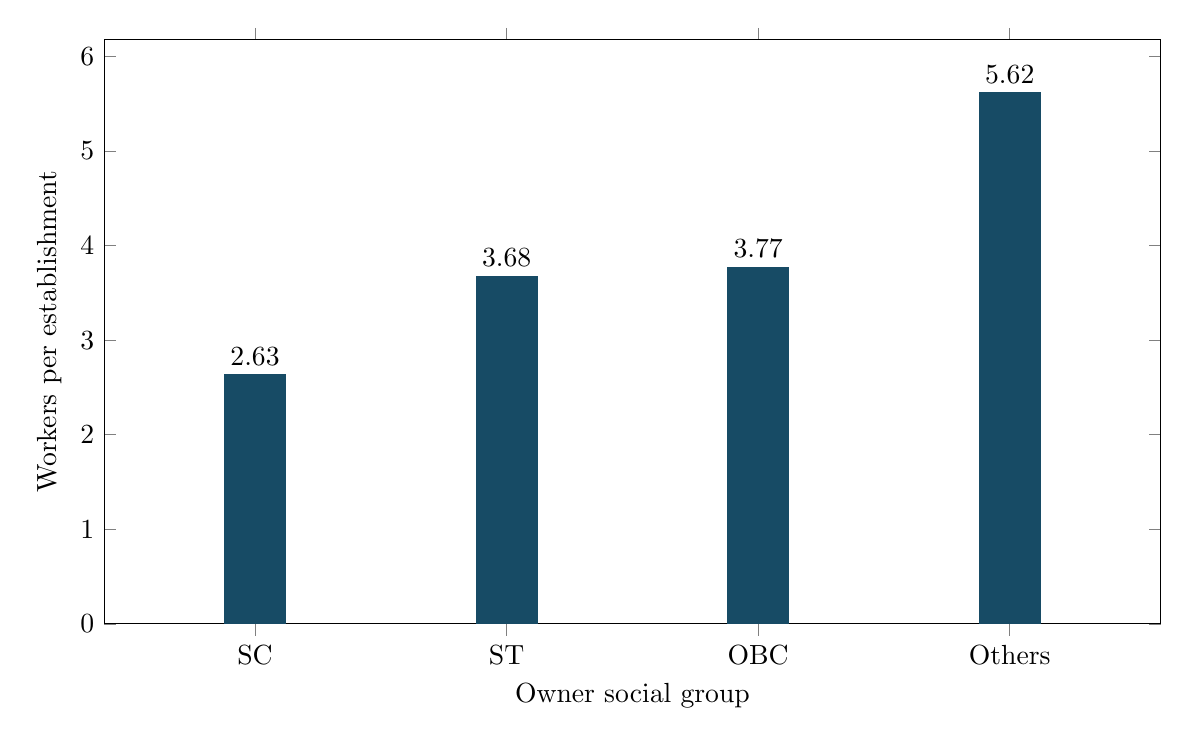
\begin{tikzpicture}
\begin{axis}[width=15cm,height=9cm,ybar,bar width=22pt,xtick={0,1,2,3},xticklabels={SC,ST,OBC,Others},ymin=0,ylabel={Workers per establishment},xlabel={Owner social group},nodes near coords,point meta=explicit symbolic,enlarge x limits=0.2]
\addplot[fill=navy,draw=navy] coordinates {(0,2.633367) [2.63] (1,3.675913) [3.68] (2,3.767702) [3.77] (3,5.615471) [5.62]};
\end{axis}
\end{tikzpicture}}

\caption{Mean employment scale by owner social group. Proprietary mining and quarrying establishments only. Source: EC6 Tables 12 and 15, PDF pages 195 and 198. Ratios of totals, not firm medians. Others is a residual category.}\end{figure}\clearpage
\clearpage\begin{figure}[p]\centering
\resizebox{\linewidth}{!}{%
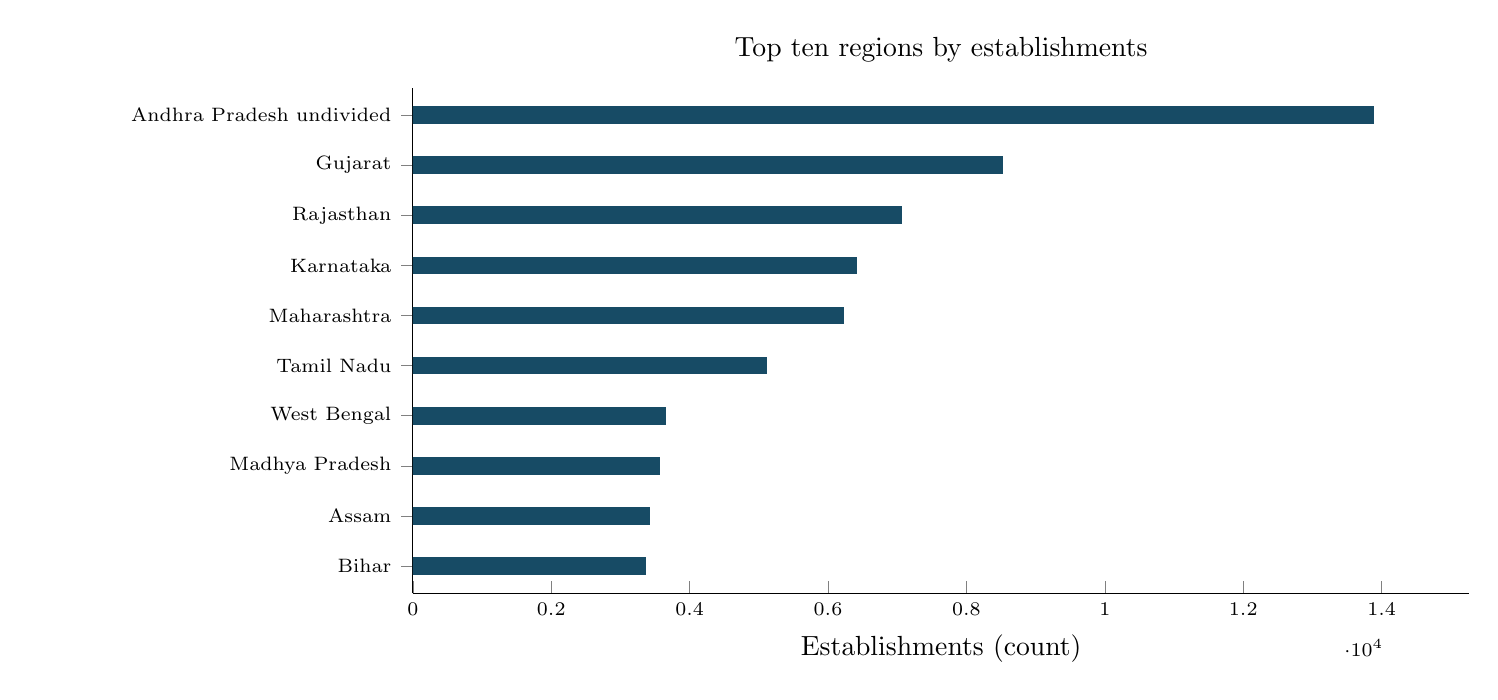
\begin{tikzpicture}
\begin{axis}[width=15cm,height=8cm,xbar,xmin=0,ytick={0,1,2,3,4,5,6,7,8,9},yticklabels={{Bihar},{Assam},{Madhya Pradesh},{West Bengal},{Tamil Nadu},{Maharashtra},{Karnataka},{Rajasthan},{Gujarat},{Andhra Pradesh undivided}},tick label style={font=\scriptsize},yticklabel style={text width=4.5cm,align=right},xlabel={Establishments (count)},title={Top ten regions by establishments},bar width=6pt,axis x line*=bottom,axis y line*=left,enlarge y limits=0.06]
\addplot[fill=navy,draw=navy] coordinates {(3368,0) (3414,1) (3564,2) (3654,3) (5110,4) (6229,5) (6406,6) (7055,7) (8516,8) (13880,9)};
\end{axis}
\end{tikzpicture}}

\par\vspace{0.5cm}
\resizebox{\linewidth}{!}{%
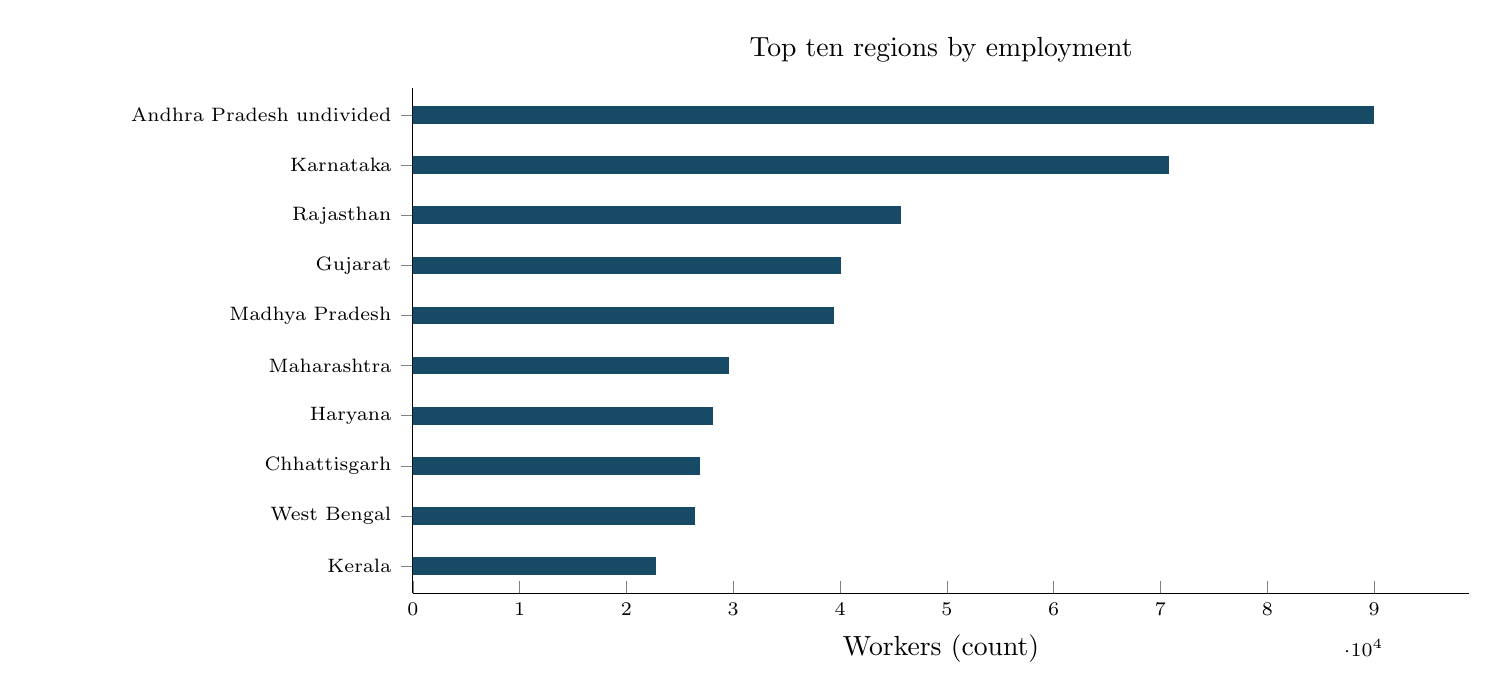
\begin{tikzpicture}
\begin{axis}[width=15cm,height=8cm,xbar,xmin=0,ytick={0,1,2,3,4,5,6,7,8,9},yticklabels={{Kerala},{West Bengal},{Chhattisgarh},{Haryana},{Maharashtra},{Madhya Pradesh},{Gujarat},{Rajasthan},{Karnataka},{Andhra Pradesh undivided}},tick label style={font=\scriptsize},yticklabel style={text width=4.5cm,align=right},xlabel={Workers (count)},title={Top ten regions by employment},bar width=6pt,axis x line*=bottom,axis y line*=left,enlarge y limits=0.06]
\addplot[fill=navy,draw=navy] coordinates {(22686,0) (26386,1) (26834,2) (28045,3) (29527,4) (39410,5) (40015,6) (45628,7) (70725,8) (89923,9)};
\end{axis}
\end{tikzpicture}}

\caption{Geographic concentration in establishments and workers. Mining and quarrying, all ownership forms. Sources: EC6 Tables 2.5 and 4.5. Undivided Andhra Pradesh combines residual Andhra Pradesh and Telangana for comparability with Census 2011.}\end{figure}\clearpage
\clearpage\begin{figure}[p]\centering
\resizebox{\linewidth}{!}{%
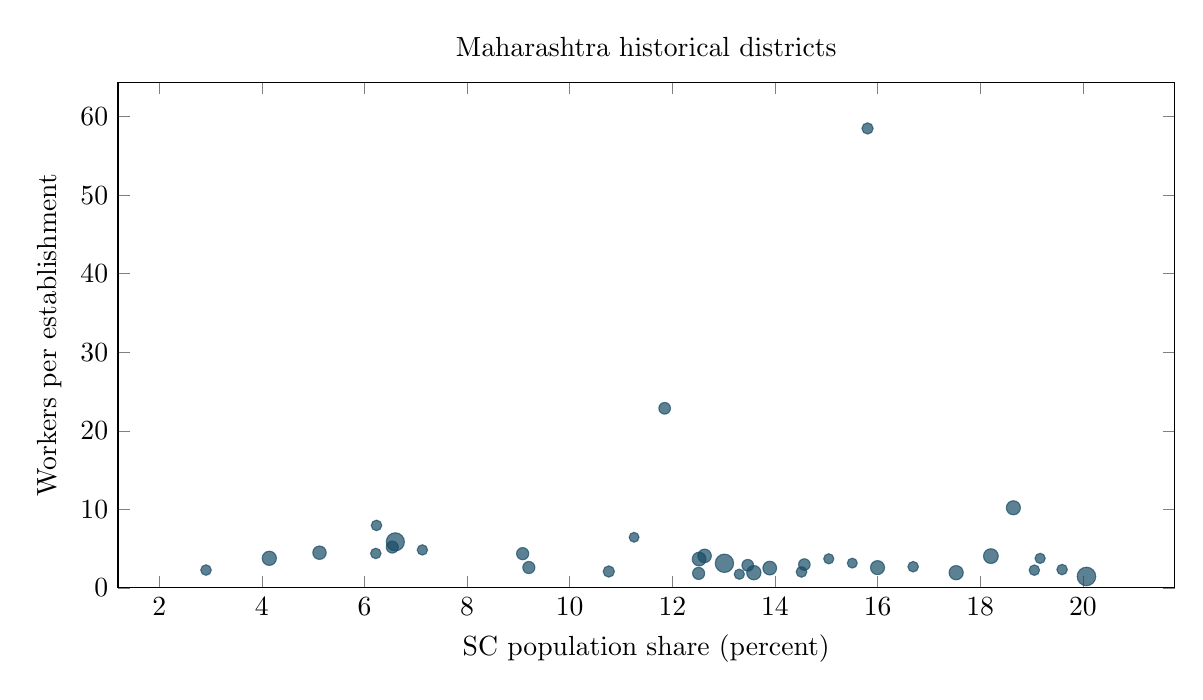
\begin{tikzpicture}
\begin{axis}[width=15cm,height=8cm,xlabel={SC population share (percent)},ylabel={Workers per establishment},title={Maharashtra historical districts},ymin=0]
\addplot[only marks,mark=*,navy,opacity=0.7,mark size=1.911pt] coordinates {(2.91119,2.270833)};
\addplot[only marks,mark=*,navy,opacity=0.7,mark size=1.898pt] coordinates {(6.22036,4.386364)};
\addplot[only marks,mark=*,navy,opacity=0.7,mark size=2.189pt] coordinates {(9.202852,2.595745)};
\addplot[only marks,mark=*,navy,opacity=0.7,mark size=2.670pt] coordinates {(18.20758,4.045181)};
\addplot[only marks,mark=*,navy,opacity=0.7,mark size=3.355pt] coordinates {(20.07044,1.455904)};
\addplot[only marks,mark=*,navy,opacity=0.7,mark size=1.849pt] coordinates {(19.1672,3.758621)};
\addplot[only marks,mark=*,navy,opacity=0.7,mark size=2.567pt] coordinates {(17.53102,1.9375)};
\addplot[only marks,mark=*,navy,opacity=0.7,mark size=1.936pt] coordinates {(14.51674,2.035714)};
\addplot[only marks,mark=*,navy,opacity=0.7,mark size=2.543pt] coordinates {(18.64618,10.20144)};
\addplot[only marks,mark=*,navy,opacity=0.7,mark size=1.904pt] coordinates {(16.69302,2.695652)};
\addplot[only marks,mark=*,navy,opacity=0.7,mark size=1.855pt] coordinates {(13.30511,1.741935)};
\addplot[only marks,mark=*,navy,opacity=0.7,mark size=1.781pt] coordinates {(11.25364,6.444444)};
\addplot[only marks,mark=*,navy,opacity=0.7,mark size=2.035pt] coordinates {(15.80383,58.5)};
\addplot[only marks,mark=*,navy,opacity=0.7,mark size=2.106pt] coordinates {(11.84981,22.86607)};
\addplot[only marks,mark=*,navy,opacity=0.7,mark size=1.895pt] coordinates {(19.05467,2.255814)};
\addplot[only marks,mark=*,navy,opacity=0.7,mark size=1.795pt] coordinates {(15.5065,3.153846)};
\addplot[only marks,mark=*,navy,opacity=0.7,mark size=2.112pt] coordinates {(13.4693,2.877193)};
\addplot[only marks,mark=*,navy,opacity=0.7,mark size=2.482pt] coordinates {(13.89789,2.521739)};
\addplot[only marks,mark=*,navy,opacity=0.7,mark size=2.097pt] coordinates {(14.57246,2.972477)};
\addplot[only marks,mark=*,navy,opacity=0.7,mark size=2.197pt] coordinates {(9.082529,4.361111)};
\addplot[only marks,mark=*,navy,opacity=0.7,mark size=3.280pt] coordinates {(6.601078,5.863057)};
\addplot[only marks,mark=*,navy,opacity=0.7,mark size=1.904pt] coordinates {(6.233882,7.956522)};
\addplot[only marks,mark=*,navy,opacity=0.7,mark size=1.872pt] coordinates {(7.128191,4.833333)};
\addplot[only marks,mark=*,navy,opacity=0.7,mark size=2.425pt] coordinates {(5.123073,4.482609)};
\addplot[only marks,mark=*,navy,opacity=0.7,mark size=2.485pt] coordinates {(12.5215,3.669291)};
\addplot[only marks,mark=*,navy,opacity=0.7,mark size=2.455pt] coordinates {(12.62773,4.07438)};
\addplot[only marks,mark=*,navy,opacity=0.7,mark size=2.586pt] coordinates {(13.5879,1.939189)};
\addplot[only marks,mark=*,navy,opacity=0.7,mark size=1.901pt] coordinates {(19.59554,2.333333)};
\addplot[only marks,mark=*,navy,opacity=0.7,mark size=2.536pt] coordinates {(15.9983,2.581818)};
\addplot[only marks,mark=*,navy,opacity=0.7,mark size=1.842pt] coordinates {(15.04821,3.703704)};
\addplot[only marks,mark=*,navy,opacity=0.7,mark size=2.041pt] coordinates {(10.76111,2.088889)};
\addplot[only marks,mark=*,navy,opacity=0.7,mark size=2.567pt] coordinates {(4.14521,3.767361)};
\addplot[only marks,mark=*,navy,opacity=0.7,mark size=2.169pt] coordinates {(6.542216,5.19403)};
\addplot[only marks,mark=*,navy,opacity=0.7,mark size=3.319pt] coordinates {(13.01499,3.132512)};
\addplot[only marks,mark=*,navy,opacity=0.7,mark size=2.191pt] coordinates {(12.51152,1.84507)};

\end{axis}
\end{tikzpicture}}

\par\vspace{0.3cm}
\resizebox{\linewidth}{!}{%
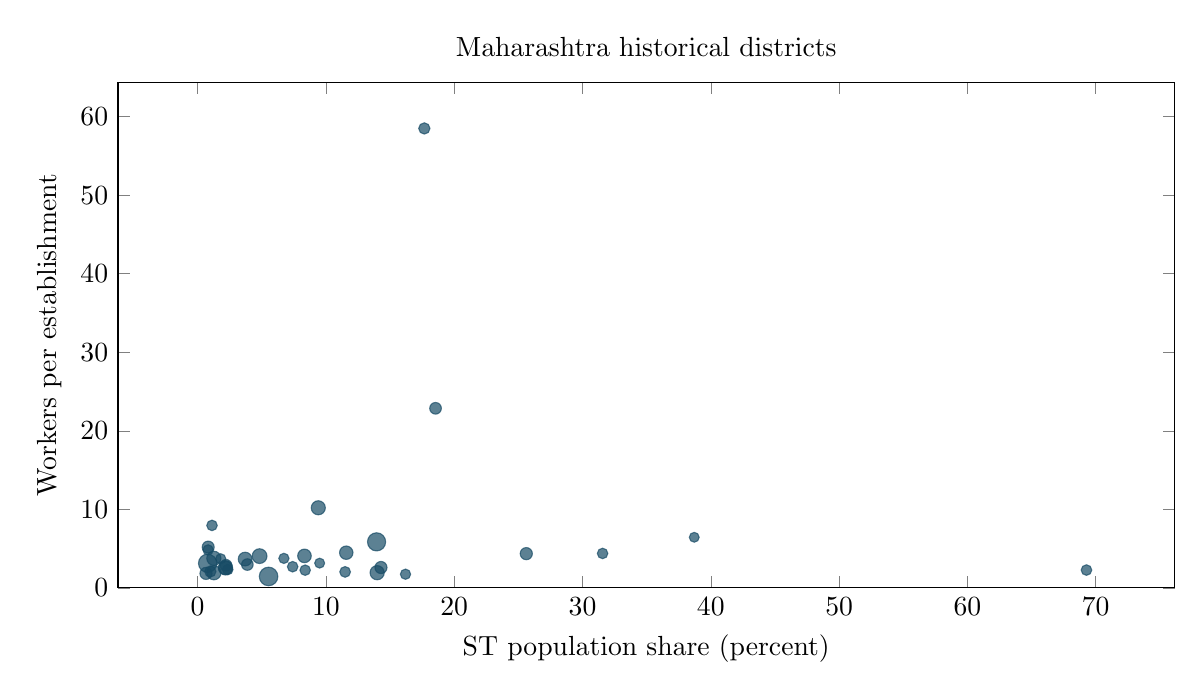
\begin{tikzpicture}
\begin{axis}[width=15cm,height=8cm,xlabel={ST population share (percent)},ylabel={Workers per establishment},title={Maharashtra historical districts},ymin=0]
\addplot[only marks,mark=*,navy,opacity=0.7,mark size=1.911pt] coordinates {(69.27965,2.270833)};
\addplot[only marks,mark=*,navy,opacity=0.7,mark size=1.898pt] coordinates {(31.56307,4.386364)};
\addplot[only marks,mark=*,navy,opacity=0.7,mark size=2.189pt] coordinates {(14.28792,2.595745)};
\addplot[only marks,mark=*,navy,opacity=0.7,mark size=2.670pt] coordinates {(4.826935,4.045181)};
\addplot[only marks,mark=*,navy,opacity=0.7,mark size=3.355pt] coordinates {(5.528401,1.455904)};
\addplot[only marks,mark=*,navy,opacity=0.7,mark size=1.849pt] coordinates {(6.721825,3.758621)};
\addplot[only marks,mark=*,navy,opacity=0.7,mark size=2.567pt] coordinates {(13.9912,1.9375)};
\addplot[only marks,mark=*,navy,opacity=0.7,mark size=1.936pt] coordinates {(11.4937,2.035714)};
\addplot[only marks,mark=*,navy,opacity=0.7,mark size=2.543pt] coordinates {(9.40291,10.20144)};
\addplot[only marks,mark=*,navy,opacity=0.7,mark size=1.904pt] coordinates {(7.405106,2.695652)};
\addplot[only marks,mark=*,navy,opacity=0.7,mark size=1.855pt] coordinates {(16.20052,1.741935)};
\addplot[only marks,mark=*,navy,opacity=0.7,mark size=1.781pt] coordinates {(38.70722,6.444444)};
\addplot[only marks,mark=*,navy,opacity=0.7,mark size=2.035pt] coordinates {(17.66728,58.5)};
\addplot[only marks,mark=*,navy,opacity=0.7,mark size=2.106pt] coordinates {(18.5423,22.86607)};
\addplot[only marks,mark=*,navy,opacity=0.7,mark size=1.895pt] coordinates {(8.380557,2.255814)};
\addplot[only marks,mark=*,navy,opacity=0.7,mark size=1.795pt] coordinates {(9.509022,3.153846)};
\addplot[only marks,mark=*,navy,opacity=0.7,mark size=2.112pt] coordinates {(2.206542,2.877193)};
\addplot[only marks,mark=*,navy,opacity=0.7,mark size=2.482pt] coordinates {(2.157326,2.521739)};
\addplot[only marks,mark=*,navy,opacity=0.7,mark size=2.097pt] coordinates {(3.873415,2.972477)};
\addplot[only marks,mark=*,navy,opacity=0.7,mark size=2.197pt] coordinates {(25.61521,4.361111)};
\addplot[only marks,mark=*,navy,opacity=0.7,mark size=3.280pt] coordinates {(13.94602,5.863057)};
\addplot[only marks,mark=*,navy,opacity=0.7,mark size=1.904pt] coordinates {(1.117457,7.956522)};
\addplot[only marks,mark=*,navy,opacity=0.7,mark size=1.872pt] coordinates {(0.813279,4.833333)};
\addplot[only marks,mark=*,navy,opacity=0.7,mark size=2.425pt] coordinates {(11.58321,4.482609)};
\addplot[only marks,mark=*,navy,opacity=0.7,mark size=2.485pt] coordinates {(3.699872,3.669291)};
\addplot[only marks,mark=*,navy,opacity=0.7,mark size=2.455pt] coordinates {(8.325264,4.07438)};
\addplot[only marks,mark=*,navy,opacity=0.7,mark size=2.586pt] coordinates {(1.265817,1.939189)};
\addplot[only marks,mark=*,navy,opacity=0.7,mark size=1.901pt] coordinates {(2.342437,2.333333)};
\addplot[only marks,mark=*,navy,opacity=0.7,mark size=2.536pt] coordinates {(2.174199,2.581818)};
\addplot[only marks,mark=*,navy,opacity=0.7,mark size=1.842pt] coordinates {(1.797045,3.703704)};
\addplot[only marks,mark=*,navy,opacity=0.7,mark size=2.041pt] coordinates {(0.986603,2.088889)};
\addplot[only marks,mark=*,navy,opacity=0.7,mark size=2.567pt] coordinates {(1.261494,3.767361)};
\addplot[only marks,mark=*,navy,opacity=0.7,mark size=2.169pt] coordinates {(0.821043,5.19403)};
\addplot[only marks,mark=*,navy,opacity=0.7,mark size=3.319pt] coordinates {(0.7793084,3.132512)};
\addplot[only marks,mark=*,navy,opacity=0.7,mark size=2.191pt] coordinates {(0.6496127,1.84507)};

\end{axis}
\end{tikzpicture}}

\par\vspace{0.3cm}
\caption{District population composition and mining establishment scale. Each point is one of 35 historical Maharashtra districts; marker area increases with establishment count. Sources: Maharashtra EC6 and Census 2011 PCA. Population shares are contextual variables, not owner identities or caste relationships. Chandrapur has mean size 58.5.}\end{figure}\clearpage
\clearpage\begin{figure}[p]\centering
\resizebox{\linewidth}{!}{%
\begin{tikzpicture}
\begin{axis}[width=15cm,height=11cm,ytick={0,1,2,3,4,5,6,7},yticklabels={{S2 SC},{S2 ST},{S3 SC},{S3 ST},{D1 SC},{D1 ST},{D4 SC},{D4 ST}},y dir=reverse,tick label style={font=\scriptsize},xlabel={Coefficient per 10 percentage points},title={Selected adjusted log-size specifications},enlarge y limits=0.08]
\addplot[gray,dashed,mark=none] coordinates {(0,-0.5)(0,7.5)};
\addplot+[only marks,mark=*,navy,error bars/.cd,x dir=both,x explicit,error bar style={navy}] coordinates {(0.03061465,0) +- (0.5238001,0) (0.008391072,1) +- (0.1505302,0) (0.1783876,2) +- (0.7081318,0) (0.03351971,3) +- (0.1630708,0) (-0.04060918,4) +- (0.6354137,0) (0.1272612,5) +- (0.3957869,0) (-0.03925949,6) +- (0.977243,0) (0.6111745,7) +- (0.9958295,0)};
\end{axis}
\end{tikzpicture}}

\caption{Selected SC and ST population-composition coefficients with 95 percent HC3 intervals. S2 all nonempty state/\allowbreak{}UT regions; S3 excludes 2011 UTs; D1 all Maharashtra districts; D4 districts with at least 50 mining establishments. Outcome is log workers per establishment. Intervals are model-based, not census sampling errors.}\end{figure}\clearpage
\clearpage\begin{figure}[p]\centering
\resizebox{\linewidth}{!}{%
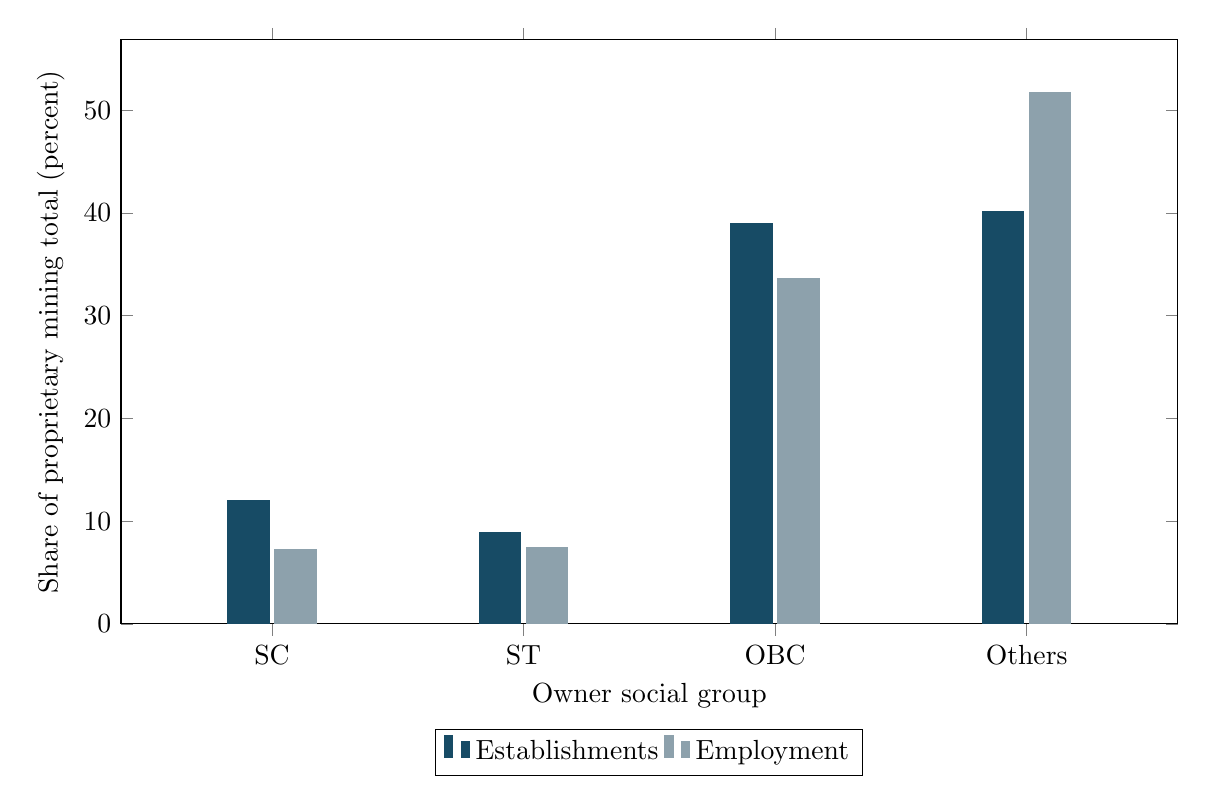
\begin{tikzpicture}
\begin{axis}[width=15cm,height=9cm,ybar,bar width=15pt,xtick={0,1,2,3},xticklabels={SC,ST,OBC,Others},ymin=0,ylabel={Share of proprietary mining total (percent)},xlabel={Owner social group},legend style={at={(0.5,-0.18)},anchor=north,legend columns=2},enlarge x limits=0.2]
\addplot[fill=navy,draw=navy] coordinates {(0,12.02542) (1,8.868389) (2,38.92989) (3,40.1763)};
\addlegendentry{Establishments}
\addplot[fill=muted,draw=muted] coordinates {(0,7.253972) (1,7.467481) (2,33.59881) (3,51.67974)};
\addlegendentry{Employment}

\end{axis}
\end{tikzpicture}}

\caption{Owner-group shares of establishments and employment. Proprietary mining only, recomputed from exact counts. Sources: EC6 Tables 12 and 15. The lower SC employment share relative to establishment share reflects smaller aggregate employment scale.}\end{figure}\clearpage
\clearpage\begin{figure}[p]\centering
\resizebox{\linewidth}{!}{%
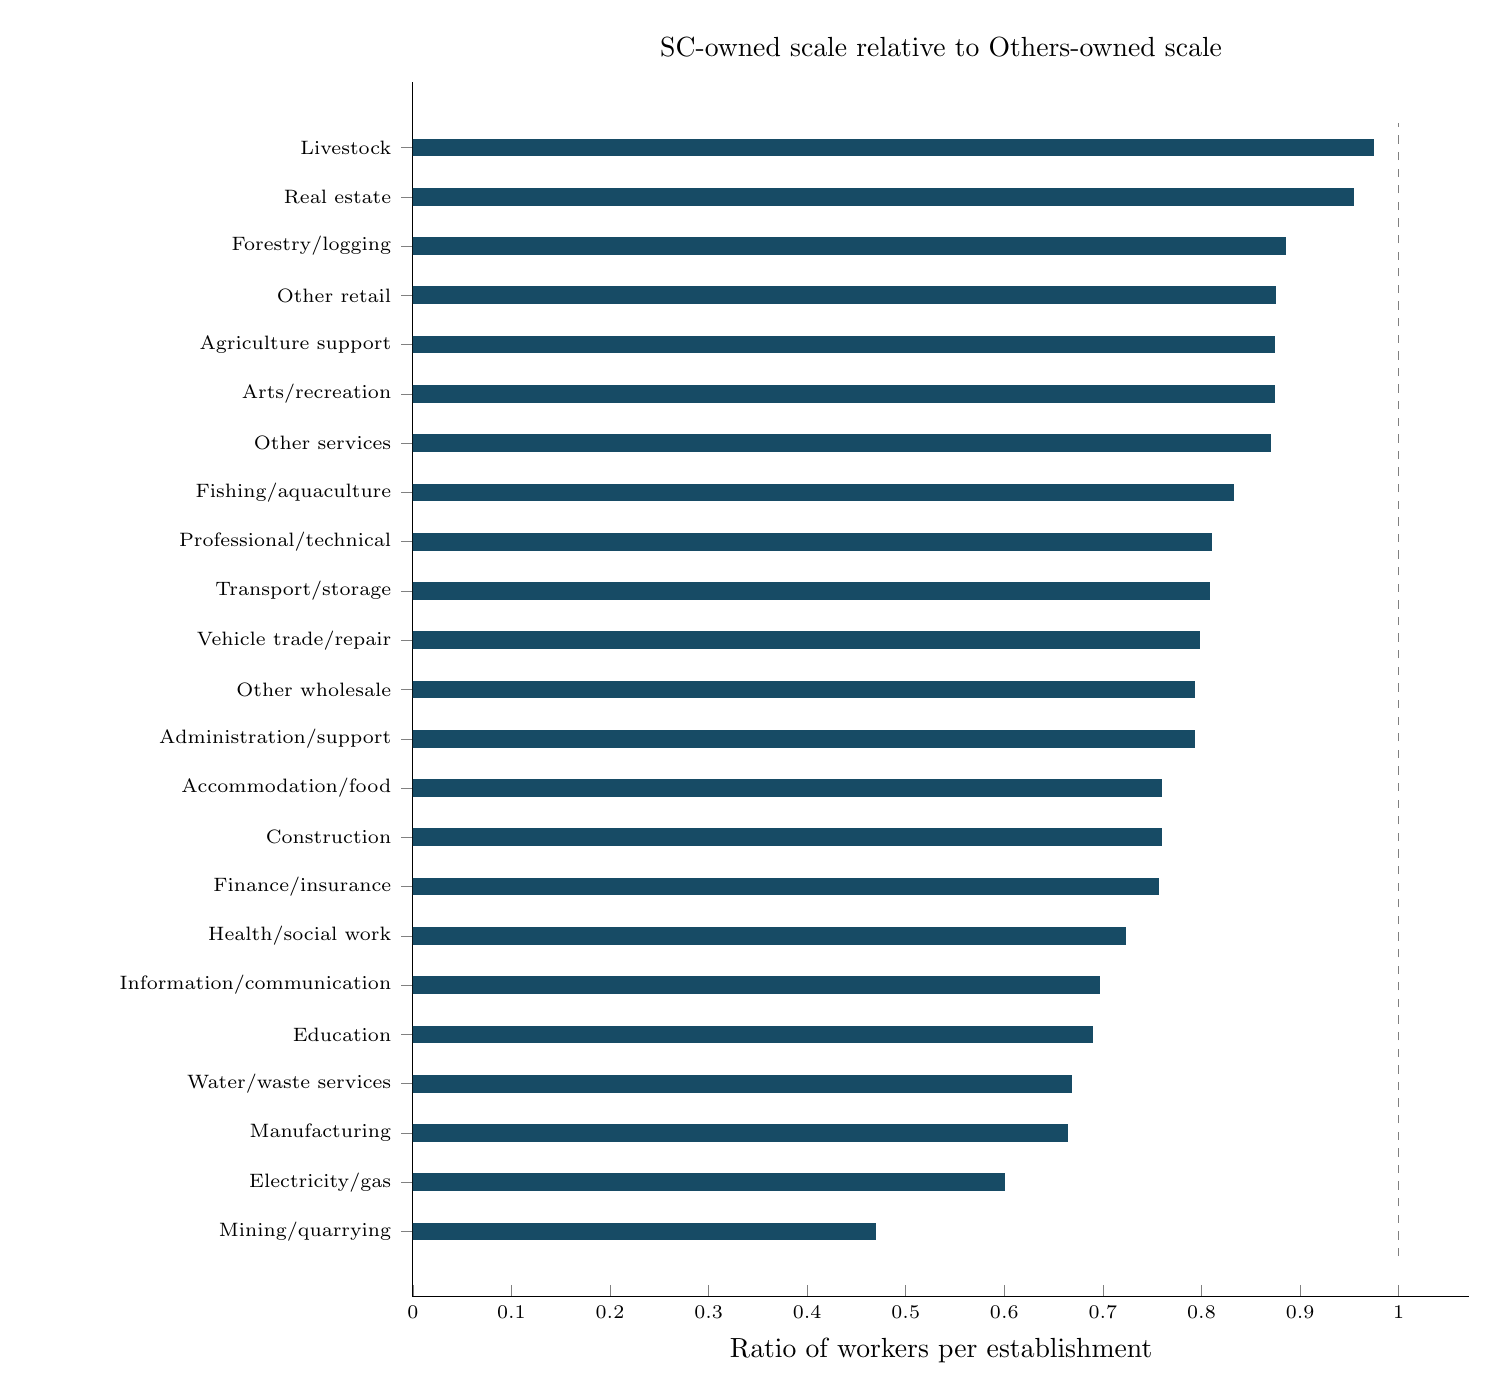
\begin{tikzpicture}
\begin{axis}[width=15cm,height=17cm,xbar,xmin=0,ytick={0,1,2,3,4,5,6,7,8,9,10,11,12,13,14,15,16,17,18,19,20,21,22},yticklabels={{Mining/\allowbreak{}quarrying},{Electricity/\allowbreak{}gas},{Manufacturing},{Water/\allowbreak{}waste services},{Education},{Information/\allowbreak{}communication},{Health/\allowbreak{}social work},{Finance/\allowbreak{}insurance},{Construction},{Accommodation/\allowbreak{}food},{Administration/\allowbreak{}support},{Other wholesale},{Vehicle trade/\allowbreak{}repair},{Transport/\allowbreak{}storage},{Professional/\allowbreak{}technical},{Fishing/\allowbreak{}aquaculture},{Other services},{Arts/\allowbreak{}recreation},{Agriculture support},{Other retail},{Forestry/\allowbreak{}logging},{Real estate},{Livestock}},tick label style={font=\scriptsize},yticklabel style={text width=4.5cm,align=right},xlabel={Ratio of workers per establishment},title={SC-owned scale relative to Others-owned scale},bar width=6pt,axis x line*=bottom,axis y line*=left,enlarge y limits=0.06]
\addplot[fill=navy,draw=navy] coordinates {(0.4689486,0) (0.6000585,1) (0.6641397,2) (0.6680537,3) (0.6895871,4) (0.696529,5) (0.7223919,6) (0.7568258,7) (0.7590394,8) (0.7596603,9) (0.7929095,10) (0.7933498,11) (0.7975721,12) (0.8077522,13) (0.8099771,14) (0.8328899,15) (0.8702429,16) (0.8736276,17) (0.8739518,18) (0.8751842,19) (0.884817,20) (0.9538043,21) (0.9743228,22)};
\draw[gray,dashed] (axis cs:1,-0.5)--(axis cs:1,22.5);\end{axis}
\end{tikzpicture}}

\caption{Cross-industry SC to Others mean-size ratios for 23 EC6 broad industries. Proprietary establishments only. Sources: Tables 12 and 15. A ratio of one is equal aggregate scale. Sector labels are shortened; full names appear in the complete industry-cell table. These are broad-sector cells, not adjusted firm-level treatment effects; mining is the Mining/\allowbreak{}quarrying row.}\end{figure}\clearpage
\clearpage\begin{figure}[p]\centering
\resizebox{\linewidth}{!}{%
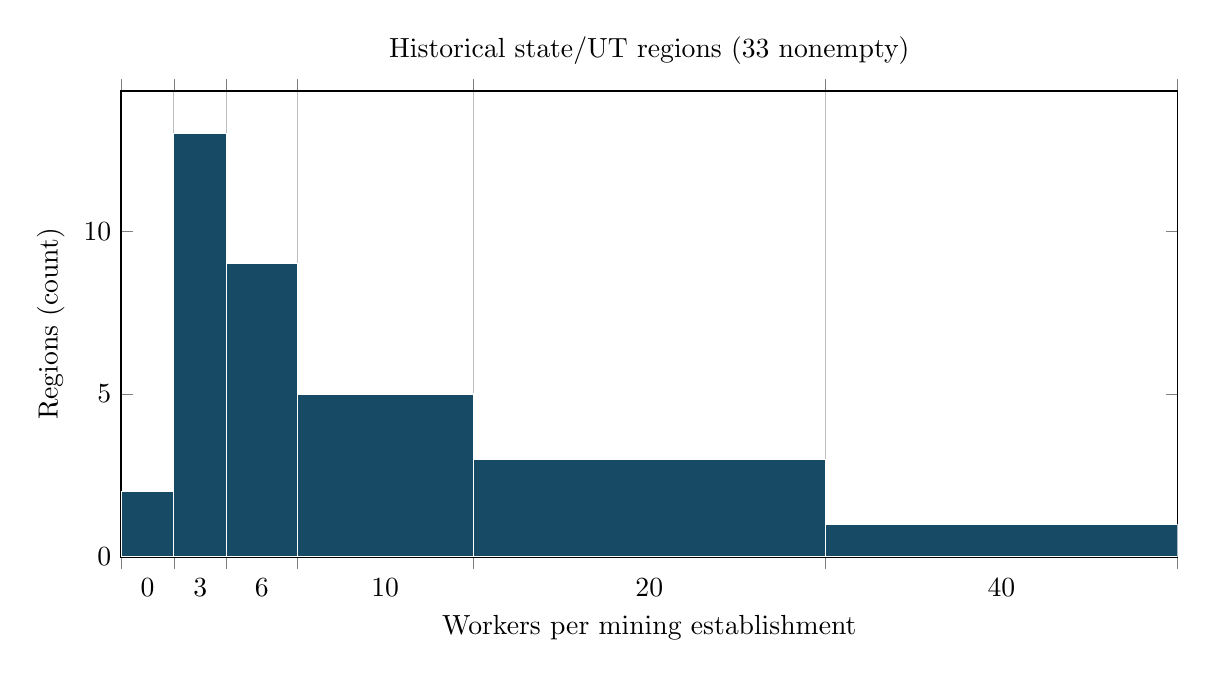
\begin{tikzpicture}
\begin{axis}[width=15cm,height=7.5cm,ybar interval,xtick={0,3,6,10,20,40,60},xmin=0,xmax=60,ymin=0,xlabel={Workers per mining establishment},ylabel={Regions (count)},title={Historical state/UT regions (33 nonempty)}]
\addplot[fill=navy,draw=white] coordinates {(0,2) (3,13) (6,9) (10,5) (20,3) (40,1) (60,0)};
\end{axis}
\end{tikzpicture}}

\par\vspace{0.3cm}
\resizebox{\linewidth}{!}{%
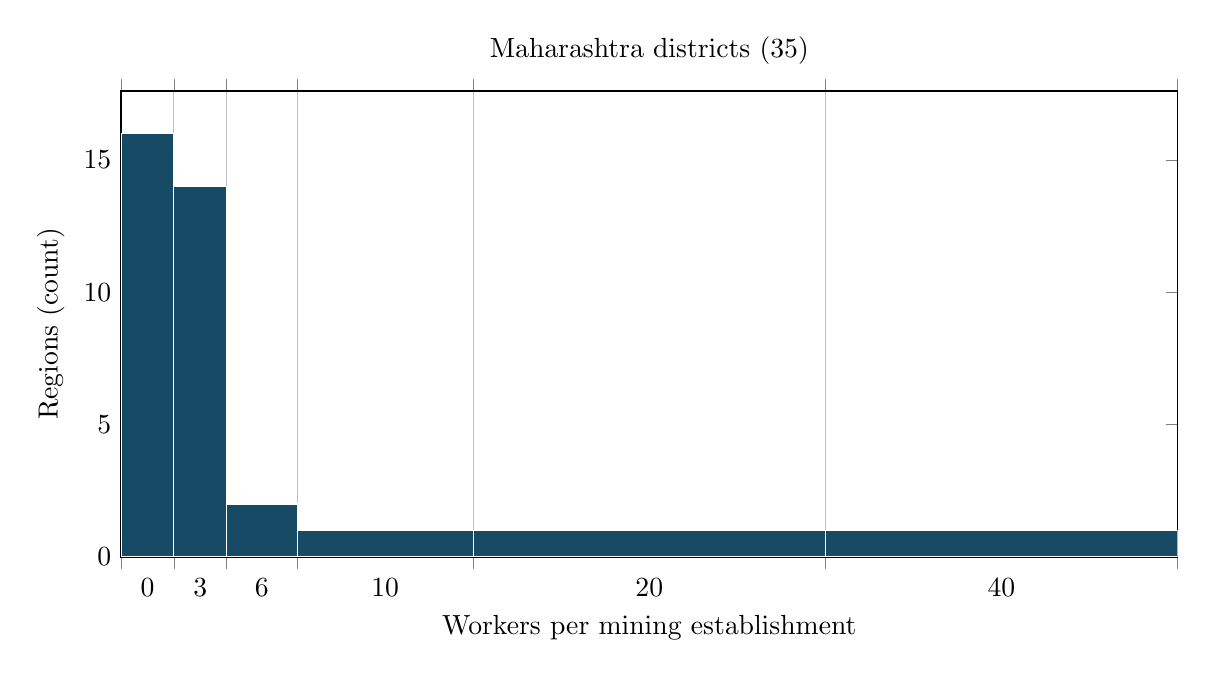
\begin{tikzpicture}
\begin{axis}[width=15cm,height=7.5cm,ybar interval,xtick={0,3,6,10,20,40,60},xmin=0,xmax=60,ymin=0,xlabel={Workers per mining establishment},ylabel={Regions (count)},title={Maharashtra districts (35)}]
\addplot[fill=navy,draw=white] coordinates {(0,16) (3,14) (6,2) (10,1) (20,1) (40,1) (60,0)};
\end{axis}
\end{tikzpicture}}

\par\vspace{0.3cm}
\caption{Distribution of regional mean sizes. EC6 mining counts and employment. These histograms describe variation in regional ratios, not a size distribution of individual firms. Bin boundaries are 0, 3, 6, 10, 20, 40 and 60 workers per establishment.}\end{figure}\clearpage
\clearpage\begin{figure}[p]\centering
\resizebox{\linewidth}{!}{%
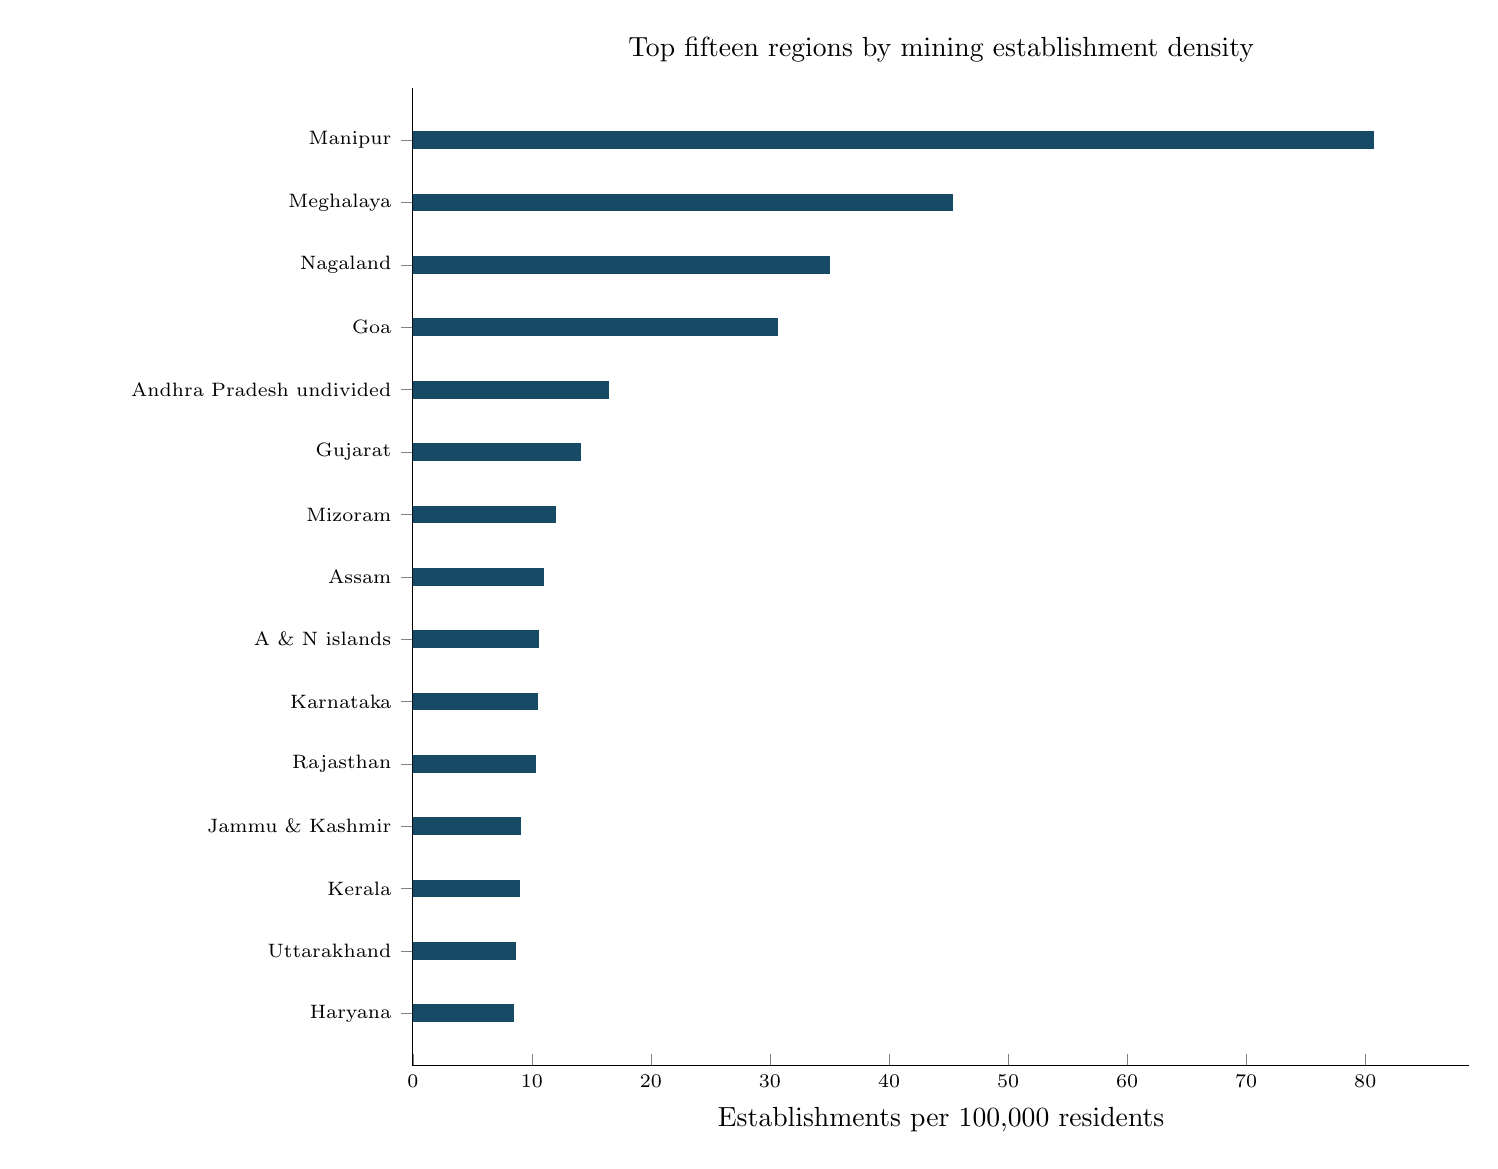
\begin{tikzpicture}
\begin{axis}[width=15cm,height=14cm,xbar,xmin=0,ytick={0,1,2,3,4,5,6,7,8,9,10,11,12,13,14},yticklabels={{Haryana},{Uttarakhand},{Kerala},{Jammu \& Kashmir},{Rajasthan},{Karnataka},{A \& N islands},{Assam},{Mizoram},{Gujarat},{Andhra Pradesh undivided},{Goa},{Nagaland},{Meghalaya},{Manipur}},tick label style={font=\scriptsize},yticklabel style={text width=4.5cm,align=right},xlabel={Establishments per 100,000 residents},title={Top fifteen regions by mining establishment density},bar width=6pt,axis x line*=bottom,axis y line*=left,enlarge y limits=0.06]
\addplot[fill=navy,draw=navy] coordinates {(8.464995,0) (8.645397,1) (8.944485,2) (9.081992,3) (10.29199,4) (10.48526,5) (10.51025,6) (10.94035,7) (11.93942,8) (14.09008,9) (16.41035,10) (30.64698,11) (35.0265,12) (45.36739,13) (80.67809,14)};
\end{axis}
\end{tikzpicture}}

\caption{Historical mining establishment density. Sources: EC6 establishment counts and Census 2011 total population. Counts include all ownership forms; the population denominator predates EC6. Undivided Andhra Pradesh includes Telangana.}\end{figure}\clearpage
\clearpage\begin{figure}[p]\centering
\small\begin{tabular}{lrrrrrrr}\toprule
 & Size & Hired share & Density & SC share & ST share & Urban & Literacy \\
Size & \cellcolor{navy!40}1.00 & \cellcolor{navy!12}0.30 & \cellcolor{orange!11}-0.27 & \cellcolor{navy!0}0.01 & \cellcolor{orange!1}-0.01 & \cellcolor{navy!9}0.23 & \cellcolor{navy!6}0.15 \\
Hired share & \cellcolor{navy!12}0.30 & \cellcolor{navy!40}1.00 & \cellcolor{orange!14}-0.35 & \cellcolor{orange!10}-0.24 & \cellcolor{orange!1}-0.02 & \cellcolor{navy!10}0.24 & \cellcolor{navy!6}0.16 \\
Density & \cellcolor{orange!11}-0.27 & \cellcolor{orange!14}-0.35 & \cellcolor{navy!40}1.00 & \cellcolor{orange!15}-0.38 & \cellcolor{navy!13}0.31 & \cellcolor{orange!6}-0.15 & \cellcolor{orange!1}-0.02 \\
SC share & \cellcolor{navy!0}0.01 & \cellcolor{orange!10}-0.24 & \cellcolor{orange!15}-0.38 & \cellcolor{navy!40}1.00 & \cellcolor{orange!27}-0.67 & \cellcolor{orange!5}-0.12 & \cellcolor{orange!9}-0.23 \\
ST share & \cellcolor{orange!1}-0.01 & \cellcolor{orange!1}-0.02 & \cellcolor{navy!13}0.31 & \cellcolor{orange!27}-0.67 & \cellcolor{navy!40}1.00 & \cellcolor{orange!3}-0.06 & \cellcolor{navy!4}0.11 \\
Urban & \cellcolor{navy!9}0.23 & \cellcolor{navy!10}0.24 & \cellcolor{orange!6}-0.15 & \cellcolor{orange!5}-0.12 & \cellcolor{orange!3}-0.06 & \cellcolor{navy!40}1.00 & \cellcolor{navy!26}0.65 \\
Literacy & \cellcolor{navy!6}0.15 & \cellcolor{navy!6}0.16 & \cellcolor{orange!1}-0.02 & \cellcolor{orange!9}-0.23 & \cellcolor{navy!4}0.11 & \cellcolor{navy!26}0.65 & \cellcolor{navy!40}1.00 \\
\bottomrule\end{tabular}
\caption{State-level Pearson correlation heatmap. Pairwise-complete observations: 33 for pairs involving size or hired share, 35 otherwise. Blue indicates positive correlation and orange negative correlation; intensity reflects absolute magnitude. Hired share means the share of establishments with hired workers, not the share of workers who are hired. Sources: EC6 and Census 2011.}\end{figure}\clearpage
\clearpage\begin{figure}[p]\centering
\resizebox{\linewidth}{!}{%
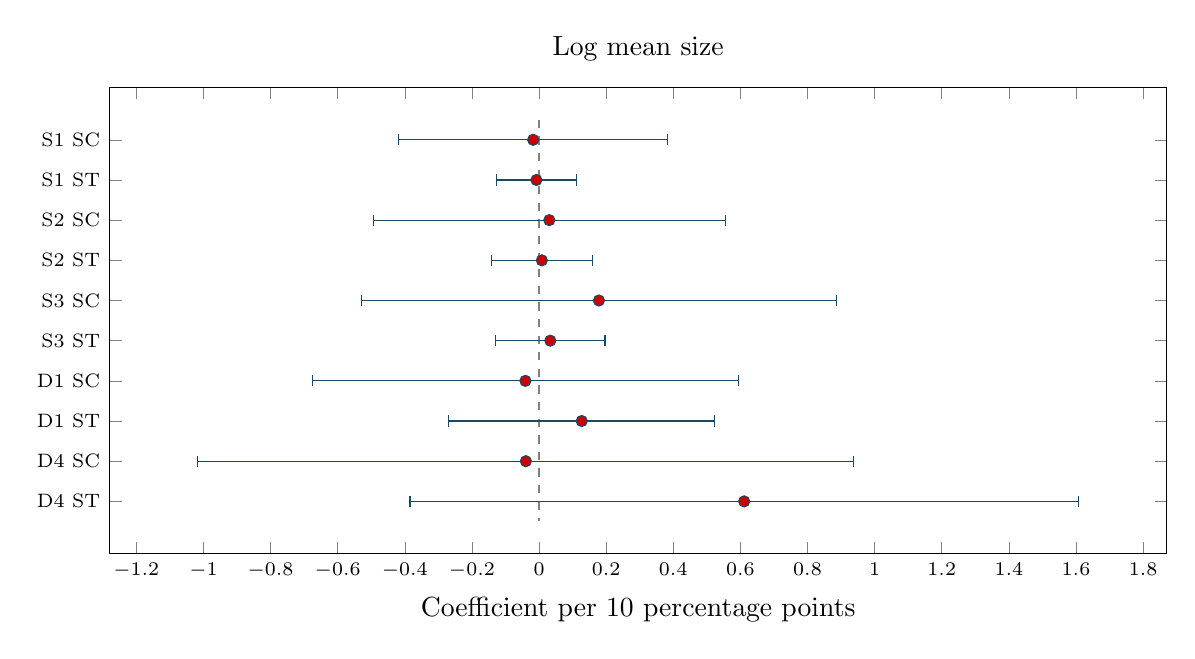
\begin{tikzpicture}
\begin{axis}[width=15cm,height=7.5cm,ytick={0,1,2,3,4,5,6,7,8,9},yticklabels={{S1 SC},{S1 ST},{S2 SC},{S2 ST},{S3 SC},{S3 ST},{D1 SC},{D1 ST},{D4 SC},{D4 ST}},y dir=reverse,tick label style={font=\scriptsize},xlabel={Coefficient per 10 percentage points},title={Log mean size},enlarge y limits=0.08]
\addplot[gray,dashed,mark=none] coordinates {(0,-0.5)(0,9.5)};
\addplot+[only marks,mark=*,navy,error bars/.cd,x dir=both,x explicit,error bar style={navy}] coordinates {(-0.01750641,0) +- (0.4011231,0) (-0.007855865,1) +- (0.1192842,0) (0.03061465,2) +- (0.5238001,0) (0.008391072,3) +- (0.1505302,0) (0.1783876,4) +- (0.7081318,0) (0.03351971,5) +- (0.1630708,0) (-0.04060918,6) +- (0.6354137,0) (0.1272612,7) +- (0.3957869,0) (-0.03925949,8) +- (0.977243,0) (0.6111745,9) +- (0.9958295,0)};
\end{axis}
\end{tikzpicture}}

\par\vspace{0.2cm}
\resizebox{\linewidth}{!}{%
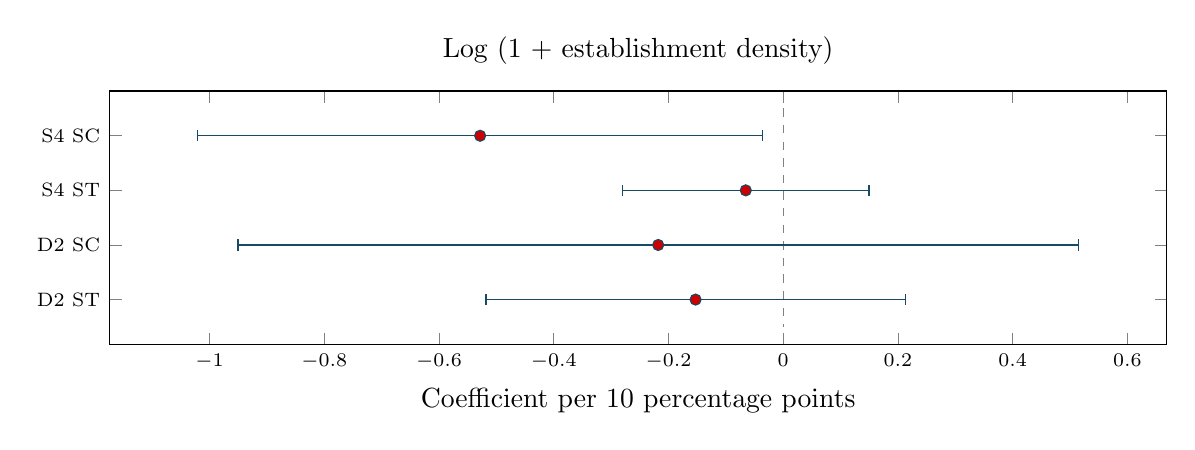
\begin{tikzpicture}
\begin{axis}[width=15cm,height=4.8cm,ytick={0,1,2,3},yticklabels={{S4 SC},{S4 ST},{D2 SC},{D2 ST}},y dir=reverse,tick label style={font=\scriptsize},xlabel={Coefficient per 10 percentage points},title={Log (1 + establishment density)},enlarge y limits=0.08]
\addplot[gray,dashed,mark=none] coordinates {(0,-0.5)(0,3.5)};
\addplot+[only marks,mark=*,navy,error bars/.cd,x dir=both,x explicit,error bar style={navy}] coordinates {(-0.528371,0) +- (0.4920177,0) (-0.06524675,1) +- (0.214796,0) (-0.2179438,2) +- (0.7325612,0) (-0.1527549,3) +- (0.3653778,0)};
\end{axis}
\end{tikzpicture}}

\par\vspace{0.2cm}
\resizebox{\linewidth}{!}{%
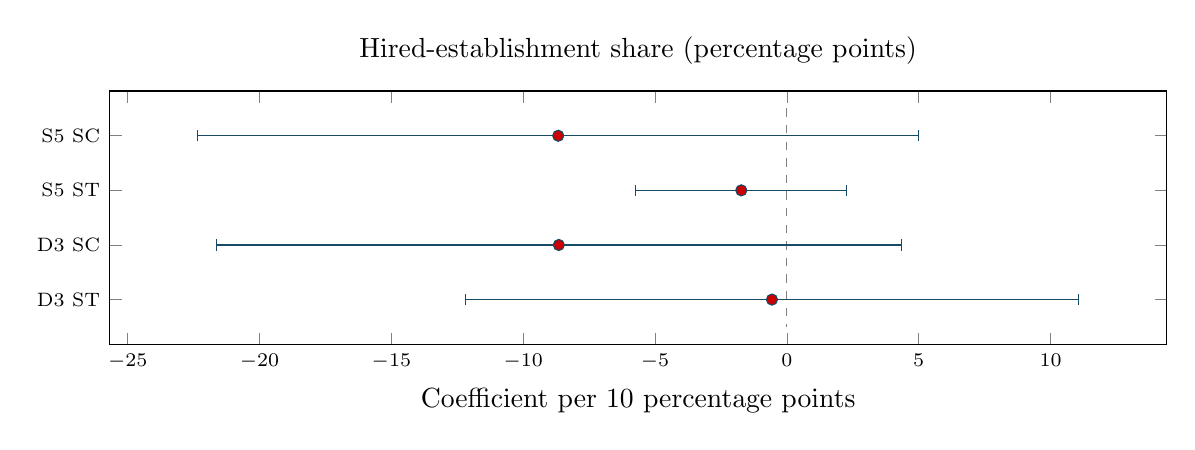
\begin{tikzpicture}
\begin{axis}[width=15cm,height=4.8cm,ytick={0,1,2,3},yticklabels={{S5 SC},{S5 ST},{D3 SC},{D3 ST}},y dir=reverse,tick label style={font=\scriptsize},xlabel={Coefficient per 10 percentage points},title={Hired-establishment share (percentage points)},enlarge y limits=0.08]
\addplot[gray,dashed,mark=none] coordinates {(0,-0.5)(0,3.5)};
\addplot+[only marks,mark=*,navy,error bars/.cd,x dir=both,x explicit,error bar style={navy}] coordinates {(-8.673576,0) +- (13.66533,0) (-1.729806,1) +- (4.003882,0) (-8.650936,2) +- (12.98568,0) (-0.5663143,3) +- (11.61997,0)};
\end{axis}
\end{tikzpicture}}

\par\vspace{0.2cm}
\caption{All 18 social-composition coefficients in nine models, with 95 percent HC3 intervals. Panels use separate outcome units; compare coefficients within an outcome, not across panels. SC/\allowbreak{}ST shares are scaled in ten percentage points. None passes the stated Holm or Benjamini--Hochberg adjustment over the 18-coefficient family.}\end{figure}\clearpage
\clearpage\begin{figure}[p]\centering
\resizebox{\linewidth}{!}{%
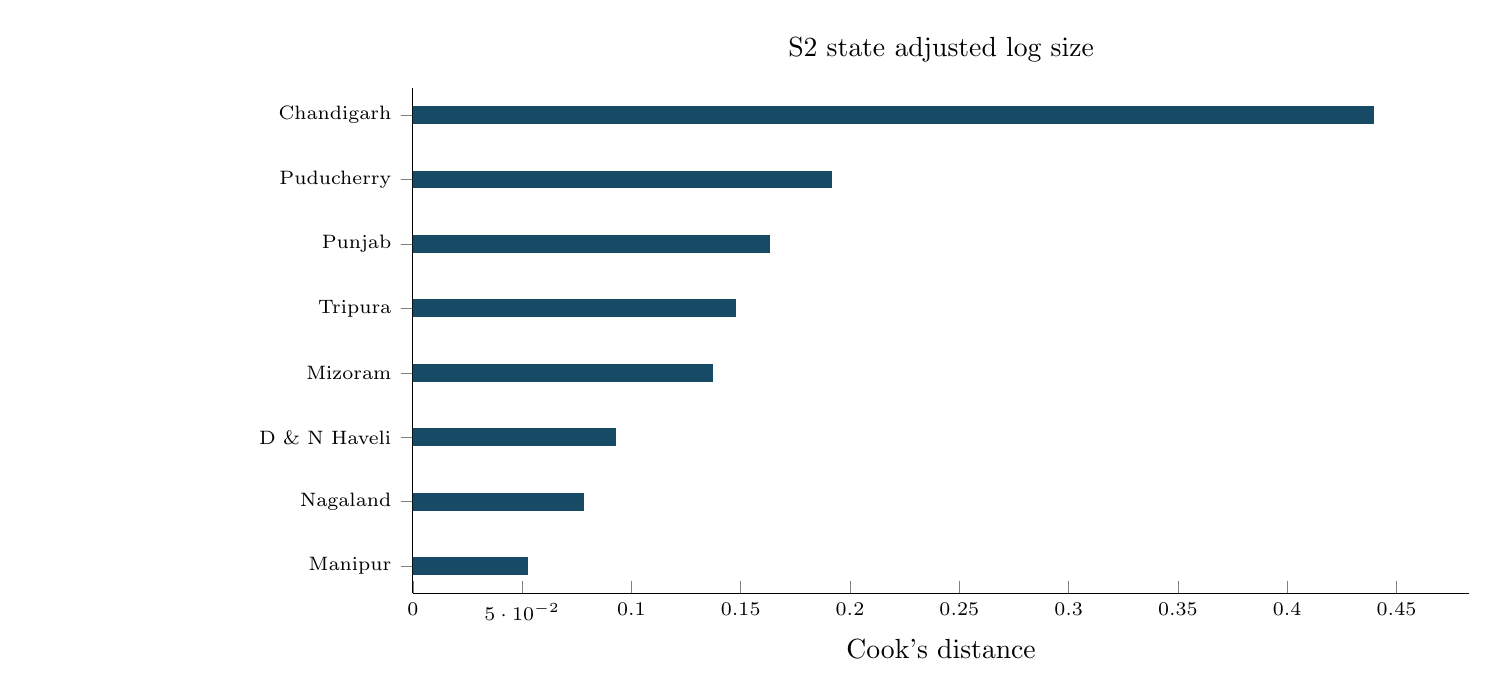
\begin{tikzpicture}
\begin{axis}[width=15cm,height=8cm,xbar,xmin=0,ytick={0,1,2,3,4,5,6,7},yticklabels={{Manipur},{Nagaland},{D \& N Haveli},{Mizoram},{Tripura},{Punjab},{Puducherry},{Chandigarh}},tick label style={font=\scriptsize},yticklabel style={text width=4.5cm,align=right},xlabel={Cook's distance},title={S2 state adjusted log size},bar width=6pt,axis x line*=bottom,axis y line*=left,enlarge y limits=0.06]
\addplot[fill=navy,draw=navy] coordinates {(0.05244097,0) (0.07801461,1) (0.09270551,2) (0.1369556,3) (0.147454,4) (0.1631666,5) (0.1912794,6) (0.4393932,7)};
\end{axis}
\end{tikzpicture}}

\par\vspace{0.3cm}
\resizebox{\linewidth}{!}{%
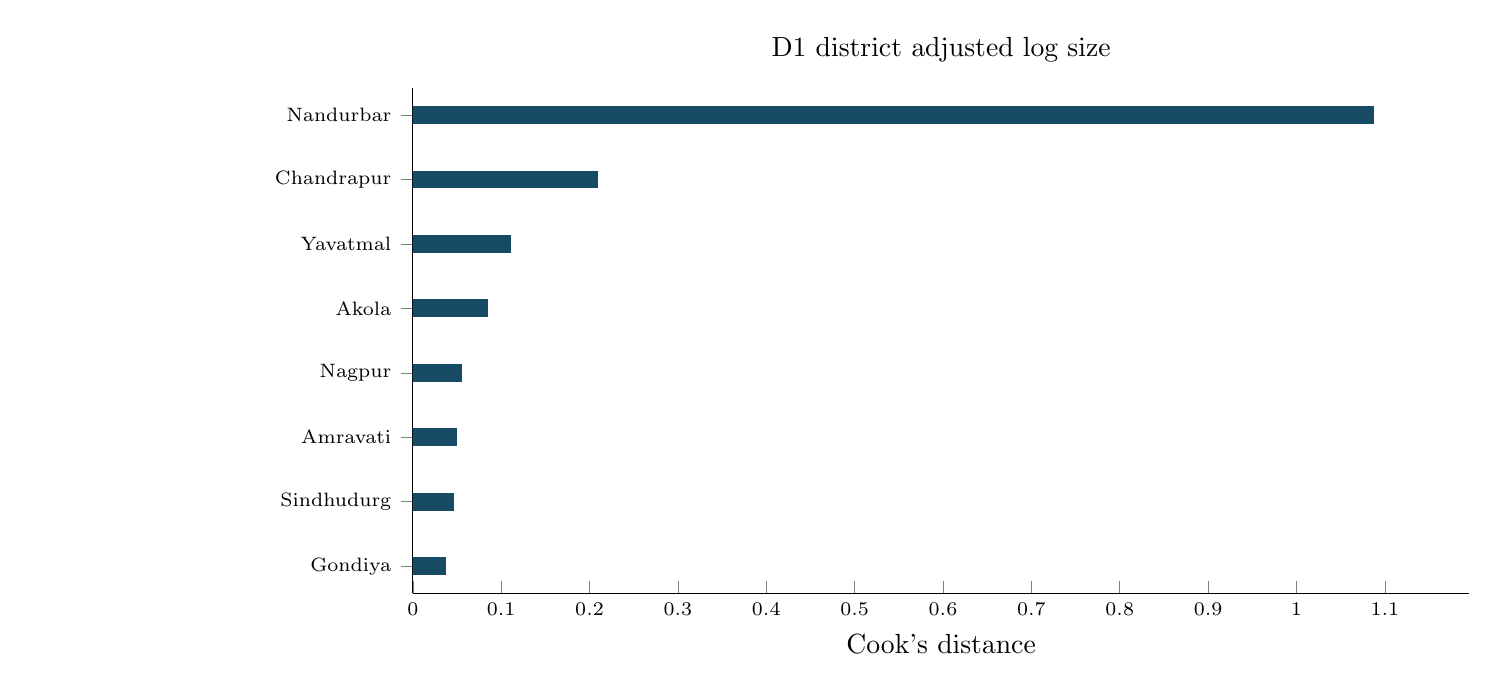
\begin{tikzpicture}
\begin{axis}[width=15cm,height=8cm,xbar,xmin=0,ytick={0,1,2,3,4,5,6,7},yticklabels={{Gondiya},{Sindhudurg},{Amravati},{Nagpur},{Akola},{Yavatmal},{Chandrapur},{Nandurbar}},tick label style={font=\scriptsize},yticklabel style={text width=4.5cm,align=right},xlabel={Cook's distance},title={D1 district adjusted log size},bar width=6pt,axis x line*=bottom,axis y line*=left,enlarge y limits=0.06]
\addplot[fill=navy,draw=navy] coordinates {(0.03734191,0) (0.04581411,1) (0.04976328,2) (0.05500545,3) (0.084754,4) (0.1100194,5) (0.2088084,6) (1.086964,7)};
\end{axis}
\end{tikzpicture}}

\par\vspace{0.3cm}
\caption{The eight most influential regions in each adjusted log-size regression. Cook's distance measures OLS sensitivity, not a probability that an observation is wrong. Full leverage, residual and leave-one-out coefficient ranges are in the statistical appendix and CSV archive.}\end{figure}\clearpage
\clearpage\begin{figure}[p]\centering
\resizebox{\linewidth}{!}{%
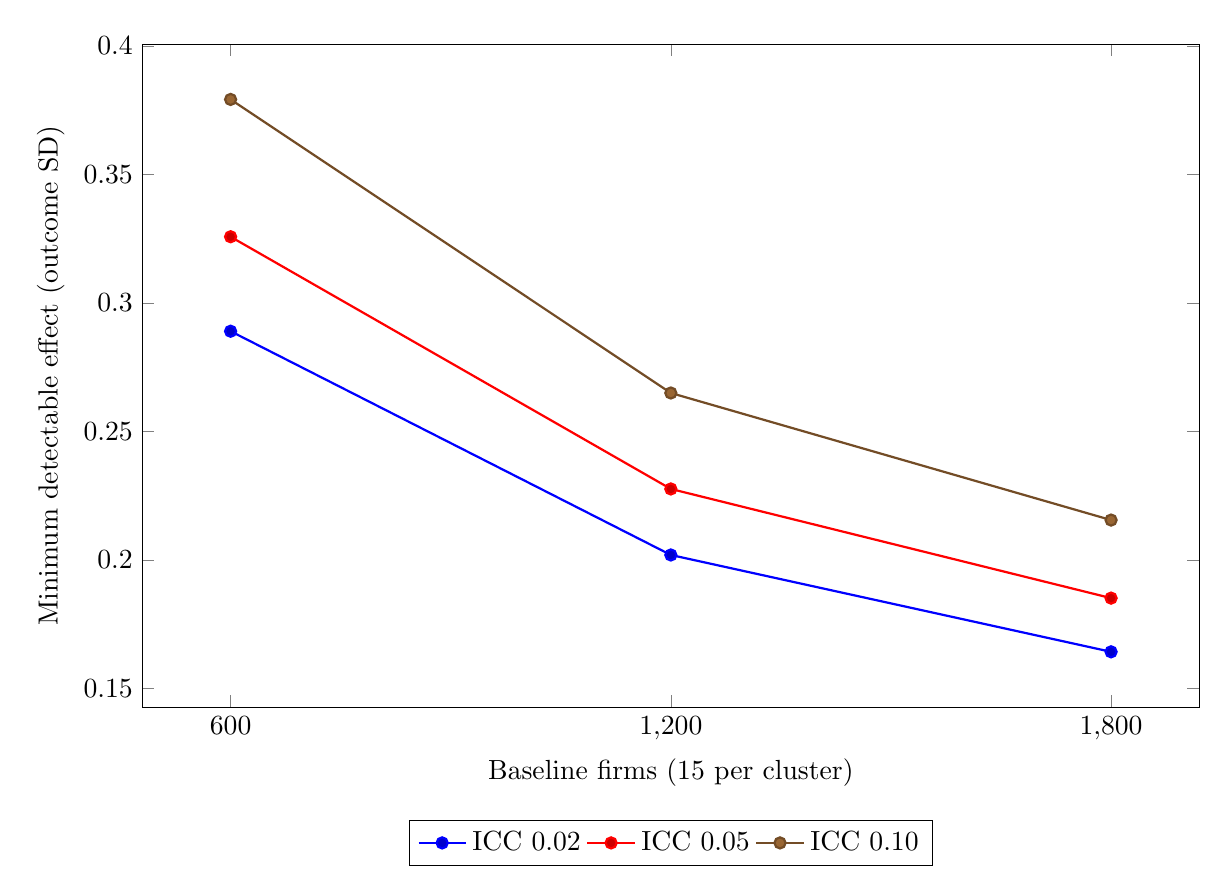
\begin{tikzpicture}
\begin{axis}[width=15cm,height=10cm,xlabel={Baseline firms (15 per cluster)},ylabel={Minimum detectable effect (outcome SD)},legend style={at={(0.5,-0.17)},anchor=north,legend columns=3},xtick={600,1200,1800}]
\addplot+[mark=*,thick] coordinates {(600,0.28898) (1200,0.2019479) (1800,0.1642742)};
\addlegendentry{ICC 0.02}
\addplot+[mark=*,thick] coordinates {(600,0.325727) (1200,0.2276278) (1800,0.1851634)};
\addlegendentry{ICC 0.05}
\addplot+[mark=*,thick] coordinates {(600,0.3791382) (1200,0.2649531) (1800,0.2155257)};
\addlegendentry{ICC 0.10}

\end{axis}
\end{tikzpicture}}

\caption{Illustrative power for a proposed cluster-randomized introduction intervention. Assumptions: 80 percent power, five percent two-sided test, equal assignment, 15 baseline firms per cluster, 20 percent attrition and the stated ICC. Retained cluster size is 12. No intervention was conducted; these are prospective design assumptions.}\end{figure}\clearpage
\chapter{Complete statistical tables}
All tables below are produced from the archived CSV files. Totals are published census tabulations; HC3 inference concerns a fitted regional model. Missing size values arise where establishment counts are zero. Rounded displays do not replace full precision in the CSV outputs.
\begingroup\footnotesize\setlength{\tabcolsep}{4pt}
\begin{longtable}{lrrrrr}
\caption{National proprietary mining ownership and employment scale}\\\toprule
Owner group & Establishments & Workers & Mean size & Est. share \% & Emp. share \% \\\midrule\endfirsthead
\multicolumn{6}{l}{\textit{Continued from previous page}}\\\toprule
Owner group & Establishments & Workers & Mean size & Est. share \% & Emp. share \% \\\midrule\endhead
\midrule\multicolumn{6}{r}{\textit{Continued on next page}}\\\endfoot\bottomrule\endlastfoot
SC & 8,799 & 23,171 & 2.63 & 12.03 & 7.25 \\
ST & 6,489 & 23,853 & 3.68 & 8.87 & 7.47 \\
OBC & 28,485 & 107,323 & 3.77 & 38.93 & 33.60 \\
Others & 29,397 & 165,078 & 5.62 & 40.18 & 51.68 \\
\end{longtable}\endgroup
\begingroup\footnotesize\setlength{\tabcolsep}{4pt}
\begin{longtable}{>{\raggedright\arraybackslash}p{5.0cm}rrrrr}
\caption{Mining establishments and employment by historical state/\allowbreak{}UT region}\\\toprule
Historical region & Estab. & Workers & Mean size & Hired \% & Density \\\midrule\endfirsthead
\multicolumn{6}{l}{\textit{Continued from previous page}}\\\toprule
Historical region & Estab. & Workers & Mean size & Hired \% & Density \\\midrule\endhead
\midrule\multicolumn{6}{r}{\textit{Continued on next page}}\\\endfoot\bottomrule\endlastfoot
Jammu \& Kashmir & 1,139 & 4,783 & 4.20 & 69.97 & 9.08 \\
Himachal Pradesh & 238 & 1,910 & 8.03 & 67.23 & 3.47 \\
Punjab & 1,207 & 2,971 & 2.46 & 49.30 & 4.35 \\
Chandigarh & 60 & 231 & 3.85 & 46.67 & 5.68 \\
Uttarakhand & 872 & 4,345 & 4.98 & 70.41 & 8.65 \\
Haryana & 2,146 & 28,045 & 13.07 & 48.56 & 8.46 \\
Delhi & 0 & 0 & -- & -- & 0.00 \\
Rajasthan & 7,055 & 45,628 & 6.47 & 66.68 & 10.29 \\
Uttar Pradesh & 3,182 & 13,959 & 4.39 & 52.51 & 1.59 \\
Bihar & 3,368 & 13,378 & 3.97 & 40.32 & 3.24 \\
Sikkim & 14 & 57 & 4.07 & 42.86 & 2.29 \\
Arunachal Pradesh & 46 & 507 & 11.02 & 65.22 & 3.32 \\
Nagaland & 693 & 2,119 & 3.06 & 36.36 & 35.03 \\
Manipur & 2,304 & 3,795 & 1.65 & 6.68 & 80.68 \\
Mizoram & 131 & 551 & 4.21 & 61.07 & 11.94 \\
Tripura & 51 & 1,089 & 21.35 & 31.37 & 1.39 \\
Meghalaya & 1,346 & 11,179 & 8.31 & 72.36 & 45.37 \\
Assam & 3,414 & 12,118 & 3.55 & 28.15 & 10.94 \\
West Bengal & 3,654 & 26,386 & 7.22 & 25.86 & 4.00 \\
Jharkhand & 2,599 & 18,067 & 6.95 & 69.22 & 7.88 \\
Odisha & 3,234 & 21,451 & 6.63 & 39.58 & 7.70 \\
Chhattisgarh & 1,188 & 26,834 & 22.59 & 72.47 & 4.65 \\
Madhya Pradesh & 3,564 & 39,410 & 11.06 & 65.88 & 4.91 \\
Gujarat & 8,516 & 40,015 & 4.70 & 72.49 & 14.09 \\
Daman \& Diu & 13 & 159 & 12.23 & 92.31 & 5.34 \\
D \& N Haveli & 11 & 303 & 27.55 & 81.82 & 3.20 \\
Maharashtra & 6,229 & 29,527 & 4.74 & 42.05 & 5.54 \\
Karnataka & 6,406 & 70,725 & 11.04 & 53.15 & 10.49 \\
Goa & 447 & 2,657 & 5.94 & 56.60 & 30.65 \\
Lakshadweep & 0 & 0 & -- & -- & 0.00 \\
Kerala & 2,988 & 22,686 & 7.59 & 81.96 & 8.94 \\
Tamil Nadu & 5,110 & 20,873 & 4.08 & 57.30 & 7.08 \\
Puducherry & 31 & 1,453 & 46.87 & 67.74 & 2.48 \\
A \& N islands & 40 & 340 & 8.50 & 92.50 & 10.51 \\
Andhra Pradesh undivided & 13,880 & 89,923 & 6.48 & 41.33 & 16.41 \\
\end{longtable}\endgroup
\begingroup\footnotesize\setlength{\tabcolsep}{4pt}
\begin{longtable}{>{\raggedright\arraybackslash}p{5.0cm}rrrrr}
\caption{State demographic controls and population denominators}\\\toprule
Historical region & Population & SC \% & ST \% & Urban \% & Literacy \% \\\midrule\endfirsthead
\multicolumn{6}{l}{\textit{Continued from previous page}}\\\toprule
Historical region & Population & SC \% & ST \% & Urban \% & Literacy \% \\\midrule\endhead
\midrule\multicolumn{6}{r}{\textit{Continued on next page}}\\\endfoot\bottomrule\endlastfoot
Jammu \& Kashmir & 12,541,302 & 7.38 & 11.91 & 27.38 & 67.16 \\
Himachal Pradesh & 6,864,602 & 25.19 & 5.71 & 10.03 & 82.80 \\
Punjab & 27,743,338 & 31.94 & 0.00 & 37.48 & 75.84 \\
Chandigarh & 1,055,450 & 18.86 & 0.00 & 97.25 & 86.05 \\
Uttarakhand & 10,086,292 & 18.76 & 2.89 & 30.23 & 78.82 \\
Haryana & 25,351,462 & 20.17 & 0.00 & 34.88 & 75.55 \\
Delhi & 16,787,941 & 16.75 & 0.00 & 97.50 & 86.21 \\
Rajasthan & 68,548,437 & 17.83 & 13.48 & 24.87 & 66.11 \\
Uttar Pradesh & 199,812,341 & 20.70 & 0.57 & 22.27 & 67.68 \\
Bihar & 104,099,452 & 15.91 & 1.28 & 11.29 & 61.80 \\
Sikkim & 610,577 & 4.63 & 33.80 & 25.15 & 81.42 \\
Arunachal Pradesh & 1,383,727 & 0.00 & 68.79 & 22.94 & 65.38 \\
Nagaland & 1,978,502 & 0.00 & 86.48 & 28.86 & 79.55 \\
Manipur & 2,855,794 & 3.41 & 40.88 & 29.21 & 76.94 \\
Mizoram & 1,097,206 & 0.11 & 94.43 & 52.11 & 91.33 \\
Tripura & 3,673,917 & 17.83 & 31.76 & 26.17 & 87.22 \\
Meghalaya & 2,966,889 & 0.58 & 86.15 & 20.07 & 74.43 \\
Assam & 31,205,576 & 7.15 & 12.45 & 14.10 & 72.19 \\
West Bengal & 91,276,115 & 23.51 & 5.80 & 31.87 & 76.26 \\
Jharkhand & 32,988,134 & 12.08 & 26.21 & 24.05 & 66.41 \\
Odisha & 41,974,218 & 17.13 & 22.85 & 16.69 & 72.87 \\
Chhattisgarh & 25,545,198 & 12.82 & 30.62 & 23.24 & 70.28 \\
Madhya Pradesh & 72,626,809 & 15.62 & 21.09 & 27.63 & 69.32 \\
Gujarat & 60,439,692 & 6.74 & 14.75 & 42.60 & 78.03 \\
Daman \& Diu & 243,247 & 2.52 & 6.32 & 75.17 & 87.10 \\
D \& N Haveli & 343,709 & 1.80 & 51.95 & 46.72 & 76.24 \\
Maharashtra & 112,374,333 & 11.81 & 9.35 & 45.22 & 82.34 \\
Karnataka & 61,095,297 & 17.15 & 6.95 & 38.67 & 75.36 \\
Goa & 1,458,545 & 1.74 & 10.23 & 62.17 & 88.70 \\
Lakshadweep & 64,473 & 0.00 & 94.80 & 78.07 & 91.85 \\
Kerala & 33,406,061 & 9.10 & 1.45 & 47.70 & 94.00 \\
Tamil Nadu & 72,147,030 & 20.01 & 1.10 & 48.40 & 80.09 \\
Puducherry & 1,247,953 & 15.73 & 0.00 & 68.33 & 85.85 \\
A \& N islands & 380,581 & 0.00 & 7.50 & 37.70 & 86.63 \\
Andhra Pradesh undivided & 84,580,777 & 16.41 & 7.00 & 33.36 & 67.02 \\
\end{longtable}\endgroup
\begingroup\footnotesize\setlength{\tabcolsep}{4pt}
\begin{longtable}{lrrrrr}
\caption{Maharashtra historical district mining establishments and employment}\\\toprule
District & Estab. & Workers & Mean size & Hired \% & Density \\\midrule\endfirsthead
\multicolumn{6}{l}{\textit{Continued from previous page}}\\\toprule
District & Estab. & Workers & Mean size & Hired \% & Density \\\midrule\endhead
\midrule\multicolumn{6}{r}{\textit{Continued on next page}}\\\endfoot\bottomrule\endlastfoot
Nandurbar & 48 & 109 & 2.27 & 16.67 & 2.91 \\
Dhule & 44 & 193 & 4.39 & 59.09 & 2.15 \\
Jalgaon & 141 & 366 & 2.60 & 24.82 & 3.33 \\
Buldana & 332 & 1,343 & 4.05 & 25.00 & 12.84 \\
Akola & 669 & 974 & 1.46 & 18.09 & 36.88 \\
Washim & 29 & 109 & 3.76 & 55.17 & 2.42 \\
Amravati & 288 & 558 & 1.94 & 21.18 & 9.97 \\
Wardha & 56 & 114 & 2.04 & 30.36 & 4.31 \\
Nagpur & 278 & 2,836 & 10.20 & 55.40 & 5.97 \\
Bhandara & 46 & 124 & 2.70 & 32.61 & 3.83 \\
Gondiya & 31 & 54 & 1.74 & 9.68 & 2.34 \\
Gadchiroli & 9 & 58 & 6.44 & 55.56 & 0.84 \\
Chandrapur & 88 & 5,148 & 58.50 & 62.50 & 3.99 \\
Yavatmal & 112 & 2,561 & 22.87 & 68.75 & 4.04 \\
Nanded & 43 & 97 & 2.26 & 30.23 & 1.28 \\
Hingoli & 13 & 41 & 3.15 & 38.46 & 1.10 \\
Parbhani & 114 & 328 & 2.88 & 45.61 & 6.21 \\
Jalna & 253 & 638 & 2.52 & 29.25 & 12.91 \\
Aurangabad & 109 & 324 & 2.97 & 44.04 & 2.94 \\
Nashik & 144 & 628 & 4.36 & 56.94 & 2.36 \\
Thane & 628 & 3,682 & 5.86 & 81.53 & 5.68 \\
Mumbai Suburban & 46 & 366 & 7.96 & 56.52 & 0.49 \\
Mumbai & 36 & 174 & 4.83 & 80.56 & 1.17 \\
Raigarh & 230 & 1,031 & 4.48 & 50.00 & 8.73 \\
Pune & 254 & 932 & 3.67 & 46.46 & 2.69 \\
Ahmadnagar & 242 & 986 & 4.07 & 57.85 & 5.33 \\
Bid & 296 & 574 & 1.94 & 33.78 & 11.45 \\
Latur & 45 & 105 & 2.33 & 31.11 & 1.83 \\
Osmanabad & 275 & 710 & 2.58 & 43.64 & 16.59 \\
Solapur & 27 & 100 & 3.70 & 44.44 & 0.63 \\
Satara & 90 & 188 & 2.09 & 14.44 & 3.00 \\
Ratnagiri & 288 & 1,085 & 3.77 & 43.40 & 17.83 \\
Sindhudurg & 134 & 696 & 5.19 & 54.48 & 15.77 \\
Kolhapur & 649 & 2,033 & 3.13 & 36.36 & 16.74 \\
Sangli & 142 & 262 & 1.85 & 25.35 & 5.03 \\
\end{longtable}\endgroup
\begingroup\footnotesize\setlength{\tabcolsep}{4pt}
\begin{longtable}{lrrrrr}
\caption{Maharashtra historical district demographic controls}\\\toprule
District & Population & SC \% & ST \% & Urban \% & Literacy \% \\\midrule\endfirsthead
\multicolumn{6}{l}{\textit{Continued from previous page}}\\\toprule
District & Population & SC \% & ST \% & Urban \% & Literacy \% \\\midrule\endhead
\midrule\multicolumn{6}{r}{\textit{Continued on next page}}\\\endfoot\bottomrule\endlastfoot
Nandurbar & 1,648,295 & 2.91 & 69.28 & 16.71 & 64.38 \\
Dhule & 2,050,862 & 6.22 & 31.56 & 27.84 & 72.80 \\
Jalgaon & 4,229,917 & 9.20 & 14.29 & 31.74 & 78.20 \\
Buldana & 2,586,258 & 18.21 & 4.83 & 21.22 & 83.40 \\
Akola & 1,813,906 & 20.07 & 5.53 & 39.68 & 88.05 \\
Washim & 1,197,160 & 19.17 & 6.72 & 17.66 & 83.25 \\
Amravati & 2,888,445 & 17.53 & 13.99 & 35.91 & 87.38 \\
Wardha & 1,300,774 & 14.52 & 11.49 & 32.54 & 86.99 \\
Nagpur & 4,653,570 & 18.65 & 9.40 & 68.31 & 88.39 \\
Bhandara & 1,200,334 & 16.69 & 7.41 & 19.48 & 83.76 \\
Gondiya & 1,322,507 & 13.31 & 16.20 & 17.08 & 84.95 \\
Gadchiroli & 1,072,942 & 11.25 & 38.71 & 11.00 & 74.36 \\
Chandrapur & 2,204,307 & 15.80 & 17.67 & 35.18 & 80.01 \\
Yavatmal & 2,772,348 & 11.85 & 18.54 & 21.58 & 82.82 \\
Nanded & 3,361,292 & 19.05 & 8.38 & 27.19 & 75.45 \\
Hingoli & 1,177,345 & 15.51 & 9.51 & 15.18 & 78.17 \\
Parbhani & 1,836,086 & 13.47 & 2.21 & 31.03 & 73.34 \\
Jalna & 1,959,046 & 13.90 & 2.16 & 19.27 & 71.52 \\
Aurangabad & 3,701,282 & 14.57 & 3.87 & 43.77 & 79.02 \\
Nashik & 6,107,187 & 9.08 & 25.62 & 42.53 & 82.31 \\
Thane & 11,060,148 & 6.60 & 13.95 & 76.99 & 84.53 \\
Mumbai Suburban & 9,356,962 & 6.23 & 1.12 & 100.00 & 89.91 \\
Mumbai & 3,085,411 & 7.13 & 0.81 & 100.00 & 89.21 \\
Raigarh & 2,634,200 & 5.12 & 11.58 & 36.83 & 83.14 \\
Pune & 9,429,408 & 12.52 & 3.70 & 60.99 & 86.15 \\
Ahmadnagar & 4,543,159 & 12.63 & 8.33 & 20.09 & 79.05 \\
Bid & 2,585,049 & 13.59 & 1.27 & 19.90 & 76.99 \\
Latur & 2,454,196 & 19.60 & 2.34 & 25.47 & 77.26 \\
Osmanabad & 1,657,576 & 16.00 & 2.17 & 16.96 & 78.44 \\
Solapur & 4,317,756 & 15.05 & 1.80 & 32.40 & 77.02 \\
Satara & 3,003,741 & 10.76 & 0.99 & 18.99 & 82.87 \\
Ratnagiri & 1,615,069 & 4.15 & 1.26 & 16.33 & 82.18 \\
Sindhudurg & 849,651 & 6.54 & 0.82 & 12.59 & 85.56 \\
Kolhapur & 3,876,001 & 13.01 & 0.78 & 31.73 & 81.51 \\
Sangli & 2,822,143 & 12.51 & 0.65 & 25.49 & 81.48 \\
\end{longtable}\endgroup
\begingroup\footnotesize\setlength{\tabcolsep}{4pt}
\begin{longtable}{>{\raggedright\arraybackslash}p{3.5cm}rrrrrrr}
\caption{State/\allowbreak{}UT regions: descriptive moments and quartiles}\\\toprule
Variable & N & Missing & Mean & SD & Min & Median & Max \\\midrule\endfirsthead
\multicolumn{8}{l}{\textit{Continued from previous page}}\\\toprule
Variable & N & Missing & Mean & SD & Min & Median & Max \\\midrule\endhead
\midrule\multicolumn{8}{r}{\textit{Continued on next page}}\\\endfoot\bottomrule\endlastfoot
Establishments & 35 & 0 & 2,433.60 & 3,050.32 & 0.00 & 1,207.00 & 13,880.00 \\
Workers & 35 & 0 & 15,927.83 & 20,994.82 & 0.00 & 4,783.00 & 89,923.00 \\
Mean size & 33 & 2 & 9.18 & 8.97 & 1.65 & 6.48 & 46.87 \\
Hired estab. share \% & 33 & 2 & 56.61 & 19.66 & 6.68 & 57.30 & 92.50 \\
Estab. per 100k & 35 & 0 & 11.13 & 15.50 & 0.00 & 7.08 & 80.68 \\
SC population \% & 35 & 0 & 11.75 & 8.68 & 0.00 & 12.82 & 31.94 \\
ST population \% & 35 & 0 & 23.10 & 29.27 & 0.00 & 10.23 & 94.80 \\
Urban population \% & 35 & 0 & 38.84 & 22.22 & 10.03 & 31.87 & 97.50 \\
Literacy \% & 35 & 0 & 77.85 & 8.59 & 61.80 & 76.94 & 94.00 \\
\end{longtable}\endgroup
\begingroup\footnotesize\setlength{\tabcolsep}{4pt}
\begin{longtable}{lrrrrr}
\caption{State/\allowbreak{}UT regions: distribution percentiles}\\\toprule
Variable & P10 & P25 & P50 & P75 & P90 \\\midrule\endfirsthead
\multicolumn{6}{l}{\textit{Continued from previous page}}\\\toprule
Variable & P10 & P25 & P50 & P75 & P90 \\\midrule\endhead
\midrule\multicolumn{6}{r}{\textit{Continued on next page}}\\\endfoot\bottomrule\endlastfoot
Establishments & 13.40 & 55.50 & 1,207.00 & 3,391.00 & 6,335.20 \\
Workers & 187.80 & 820.00 & 4,783.00 & 24,536.00 & 39,773.00 \\
Mean size & 3.61 & 4.20 & 6.48 & 11.02 & 19.70 \\
Hired estab. share \% & 32.37 & 42.05 & 57.30 & 69.97 & 79.95 \\
Estab. per 100k & 1.87 & 3.40 & 7.08 & 10.50 & 24.95 \\
SC population \% & 0.04 & 2.96 & 12.82 & 17.83 & 20.49 \\
ST population \% & 0.00 & 2.17 & 10.23 & 31.19 & 79.20 \\
Urban population \% & 18.04 & 24.46 & 31.87 & 47.21 & 72.44 \\
Literacy \% & 66.65 & 71.23 & 76.94 & 85.95 & 88.11 \\
\end{longtable}\endgroup
\begingroup\footnotesize\setlength{\tabcolsep}{4pt}
\begin{longtable}{>{\raggedright\arraybackslash}p{3.5cm}rrrrrrr}
\caption{Maharashtra districts: descriptive moments and quartiles}\\\toprule
Variable & N & Missing & Mean & SD & Min & Median & Max \\\midrule\endfirsthead
\multicolumn{8}{l}{\textit{Continued from previous page}}\\\toprule
Variable & N & Missing & Mean & SD & Min & Median & Max \\\midrule\endhead
\midrule\multicolumn{8}{r}{\textit{Continued on next page}}\\\endfoot\bottomrule\endlastfoot
Establishments & 35 & 0 & 177.97 & 176.80 & 9.00 & 114.00 & 669.00 \\
Workers & 35 & 0 & 843.63 & 1,136.18 & 41.00 & 366.00 & 5,148.00 \\
Mean size & 35 & 0 & 5.73 & 9.91 & 1.46 & 3.15 & 58.50 \\
Hired estab. share \% & 35 & 0 & 42.27 & 18.01 & 9.68 & 43.64 & 81.53 \\
Estab. per 100k & 35 & 0 & 6.73 & 7.35 & 0.49 & 3.99 & 36.88 \\
SC population \% & 35 & 0 & 12.64 & 4.79 & 2.91 & 13.31 & 20.07 \\
ST population \% & 35 & 0 & 10.54 & 13.69 & 0.65 & 6.72 & 69.28 \\
Urban population \% & 35 & 0 & 33.42 & 22.41 & 11.00 & 27.19 & 100.00 \\
Literacy \% & 35 & 0 & 80.97 & 5.64 & 64.38 & 82.18 & 89.91 \\
\end{longtable}\endgroup
\begingroup\footnotesize\setlength{\tabcolsep}{4pt}
\begin{longtable}{lrrrrr}
\caption{Maharashtra districts: distribution percentiles}\\\toprule
Variable & P10 & P25 & P50 & P75 & P90 \\\midrule\endfirsthead
\multicolumn{6}{l}{\textit{Continued from previous page}}\\\toprule
Variable & P10 & P25 & P50 & P75 & P90 \\\midrule\endhead
\midrule\multicolumn{6}{r}{\textit{Continued on next page}}\\\endfoot\bottomrule\endlastfoot
Establishments & 29.80 & 45.50 & 114.00 & 264.50 & 317.60 \\
Workers & 98.20 & 119.00 & 366.00 & 980.00 & 2,349.80 \\
Mean size & 1.94 & 2.30 & 3.15 & 4.43 & 7.35 \\
Hired estab. share \% & 19.32 & 29.74 & 43.64 & 55.48 & 61.14 \\
Estab. per 100k & 1.13 & 2.35 & 3.99 & 9.35 & 16.26 \\
SC population \% & 6.23 & 9.14 & 13.31 & 15.90 & 18.89 \\
ST population \% & 0.89 & 1.98 & 6.72 & 13.97 & 22.79 \\
Urban population \% & 16.48 & 19.13 & 27.19 & 36.37 & 65.38 \\
Literacy \% & 73.74 & 77.72 & 82.18 & 84.74 & 87.78 \\
\end{longtable}\endgroup
\section{Regression specifications and all coefficients}
S1: state log size, SC/ST shares only. S2: adds urban and literacy shares. S3: S2 excluding historical UTs. S4: state log(1+density), adjusted. S5: state hired-establishment share, adjusted. D1: district log size, adjusted. D2: district log(1+density), adjusted. D3: district hired-establishment share, adjusted. D4: D1 among districts with at least 50 establishments. All share regressors use ten-percentage-point units; const is the intercept.
\begingroup\footnotesize\setlength{\tabcolsep}{4pt}
\begin{longtable}{llrr}
\caption{Model sample sizes and fit}\\\toprule
Model & Outcome & N & R squared \\\midrule\endfirsthead
\multicolumn{4}{l}{\textit{Continued from previous page}}\\\toprule
Model & Outcome & N & R squared \\\midrule\endhead
\midrule\multicolumn{4}{r}{\textit{Continued on next page}}\\\endfoot\bottomrule\endlastfoot
S1 & log\_size & 33 & 0.0005 \\
S2 & log\_size & 33 & 0.0200 \\
S3 & log\_size & 28 & 0.0465 \\
S4 & log\_density & 35 & 0.2323 \\
S5 & hired\_est\_pct & 33 & 0.1375 \\
D1 & log\_size & 35 & 0.1155 \\
D2 & log\_density & 35 & 0.2149 \\
D3 & hired\_est\_pct & 35 & 0.2945 \\
D4 & log\_size & 23 & 0.2612 \\
\end{longtable}\endgroup
\begingroup\footnotesize\setlength{\tabcolsep}{4pt}
\begin{longtable}{llrrrrr}
\caption{All fitted regression coefficients and HC3 inference}\\\toprule
Model & Term & Beta & HC3 SE & t-based p & CI low & CI high \\\midrule\endfirsthead
\multicolumn{7}{l}{\textit{Continued from previous page}}\\\toprule
Model & Term & Beta & HC3 SE & t-based p & CI low & CI high \\\midrule\endhead
\midrule\multicolumn{7}{r}{\textit{Continued on next page}}\\\endfoot\bottomrule\endlastfoot
S1 & const & 1.9681 & 0.3250 & 0.0000 & 1.3044 & 2.6318 \\
S1 & sc\_10pp & -0.0175 & 0.1964 & 0.9296 & -0.4186 & 0.3836 \\
S1 & st\_10pp & -0.0079 & 0.0584 & 0.8939 & -0.1271 & 0.1114 \\
S2 & const & 1.5438 & 1.5336 & 0.3227 & -1.5977 & 4.6852 \\
S2 & sc\_10pp & 0.0306 & 0.2557 & 0.9056 & -0.4932 & 0.5544 \\
S2 & st\_10pp & 0.0084 & 0.0735 & 0.9099 & -0.1421 & 0.1589 \\
S2 & urban\_10pp & 0.0501 & 0.1515 & 0.7432 & -0.2602 & 0.3604 \\
S2 & literacy\_10pp & 0.0197 & 0.2080 & 0.9253 & -0.4063 & 0.4457 \\
S3 & const & 1.3326 & 1.4368 & 0.3633 & -1.6396 & 4.3048 \\
S3 & sc\_10pp & 0.1784 & 0.3423 & 0.6073 & -0.5297 & 0.8865 \\
S3 & st\_10pp & 0.0335 & 0.0788 & 0.6746 & -0.1296 & 0.1966 \\
S3 & urban\_10pp & -0.0459 & 0.1389 & 0.7437 & -0.3332 & 0.2413 \\
S3 & literacy\_10pp & 0.0407 & 0.2056 & 0.8447 & -0.3845 & 0.4660 \\
S4 & const & 3.2009 & 1.8138 & 0.0878 & -0.5034 & 6.9052 \\
S4 & sc\_10pp & -0.5284 & 0.2409 & 0.0362 & -1.0204 & -0.0364 \\
S4 & st\_10pp & -0.0652 & 0.1052 & 0.5397 & -0.2800 & 0.1495 \\
S4 & urban\_10pp & -0.1592 & 0.1273 & 0.2207 & -0.4191 & 0.1008 \\
S4 & literacy\_10pp & 0.0290 & 0.2402 & 0.9047 & -0.4615 & 0.5195 \\
S5 & const & 67.2899 & 39.5409 & 0.0999 & -13.7059 & 148.2857 \\
S5 & sc\_10pp & -8.6736 & 6.6712 & 0.2041 & -22.3389 & 4.9918 \\
S5 & st\_10pp & -1.7298 & 1.9546 & 0.3837 & -5.7337 & 2.2741 \\
S5 & urban\_10pp & 1.7362 & 3.5835 & 0.6318 & -5.6043 & 9.0768 \\
S5 & literacy\_10pp & -0.3628 & 6.1550 & 0.9534 & -12.9708 & 12.2453 \\
D1 & const & -0.5228 & 2.4547 & 0.8328 & -5.5359 & 4.4903 \\
D1 & sc\_10pp & -0.0406 & 0.3111 & 0.8970 & -0.6760 & 0.5948 \\
D1 & st\_10pp & 0.1273 & 0.1938 & 0.5164 & -0.2685 & 0.5230 \\
D1 & urban\_10pp & 0.0735 & 0.0600 & 0.2305 & -0.0491 & 0.1960 \\
D1 & literacy\_10pp & 0.1864 & 0.3110 & 0.5534 & -0.4487 & 0.8215 \\
D2 & const & -0.4305 & 3.2044 & 0.8940 & -6.9748 & 6.1139 \\
D2 & sc\_10pp & -0.2179 & 0.3587 & 0.5480 & -0.9505 & 0.5146 \\
D2 & st\_10pp & -0.1528 & 0.1789 & 0.4000 & -0.5181 & 0.2126 \\
D2 & urban\_10pp & -0.1683 & 0.0745 & 0.0313 & -0.3205 & -0.0161 \\
D2 & literacy\_10pp & 0.3886 & 0.3818 & 0.3170 & -0.3912 & 1.1684 \\
D3 & const & 53.7536 & 62.8033 & 0.3988 & -74.5079 & 182.0151 \\
D3 & sc\_10pp & -8.6509 & 6.3584 & 0.1838 & -21.6366 & 4.3347 \\
D3 & st\_10pp & -0.5663 & 5.6897 & 0.9214 & -12.1863 & 11.0537 \\
D3 & urban\_10pp & 3.7347 & 1.7898 & 0.0455 & 0.0795 & 7.3900 \\
D3 & literacy\_10pp & -1.5360 & 8.1623 & 0.8520 & -18.2056 & 15.1336 \\
D4 & const & 1.8579 & 3.4415 & 0.5959 & -5.3725 & 9.0883 \\
D4 & sc\_10pp & -0.0393 & 0.4651 & 0.9337 & -1.0165 & 0.9380 \\
D4 & st\_10pp & 0.6112 & 0.4740 & 0.2136 & -0.3847 & 1.6070 \\
D4 & urban\_10pp & 0.0131 & 0.1148 & 0.9106 & -0.2281 & 0.2542 \\
D4 & literacy\_10pp & -0.1172 & 0.4480 & 0.7966 & -1.0585 & 0.8241 \\
\end{longtable}\endgroup
\begingroup\footnotesize\setlength{\tabcolsep}{4pt}
\begin{longtable}{llrrr}
\caption{Multiple-testing adjustments: 18 SC/\allowbreak{}ST coefficients}\\\toprule
Model & Term & Unadj. p & Holm p & BH q \\\midrule\endfirsthead
\multicolumn{5}{l}{\textit{Continued from previous page}}\\\toprule
Model & Term & Unadj. p & Holm p & BH q \\\midrule\endhead
\midrule\multicolumn{5}{r}{\textit{Continued on next page}}\\\endfoot\bottomrule\endlastfoot
S1 & sc\_10pp & 0.9296 & 1.0000 & 0.9337 \\
S1 & st\_10pp & 0.8939 & 1.0000 & 0.9337 \\
S2 & sc\_10pp & 0.9056 & 1.0000 & 0.9337 \\
S2 & st\_10pp & 0.9099 & 1.0000 & 0.9337 \\
S3 & sc\_10pp & 0.6073 & 1.0000 & 0.9337 \\
S3 & st\_10pp & 0.6746 & 1.0000 & 0.9337 \\
S4 & sc\_10pp & 0.0362 & 0.6513 & 0.6513 \\
S4 & st\_10pp & 0.5397 & 1.0000 & 0.9337 \\
S5 & sc\_10pp & 0.2041 & 1.0000 & 0.9337 \\
S5 & st\_10pp & 0.3837 & 1.0000 & 0.9337 \\
D1 & sc\_10pp & 0.8970 & 1.0000 & 0.9337 \\
D1 & st\_10pp & 0.5164 & 1.0000 & 0.9337 \\
D2 & sc\_10pp & 0.5480 & 1.0000 & 0.9337 \\
D2 & st\_10pp & 0.4000 & 1.0000 & 0.9337 \\
D3 & sc\_10pp & 0.1838 & 1.0000 & 0.9337 \\
D3 & st\_10pp & 0.9214 & 1.0000 & 0.9337 \\
D4 & sc\_10pp & 0.9337 & 1.0000 & 0.9337 \\
D4 & st\_10pp & 0.2136 & 1.0000 & 0.9337 \\
\end{longtable}\endgroup
\begingroup\footnotesize\setlength{\tabcolsep}{4pt}
\begin{longtable}{llrr}
\caption{Leave-one-region-out coefficient ranges}\\\toprule
Model & Term & Minimum beta & Maximum beta \\\midrule\endfirsthead
\multicolumn{4}{l}{\textit{Continued from previous page}}\\\toprule
Model & Term & Minimum beta & Maximum beta \\\midrule\endhead
\midrule\multicolumn{4}{r}{\textit{Continued on next page}}\\\endfoot\bottomrule\endlastfoot
S1 & sc\_10pp & -0.0875 & 0.1250 \\
S1 & st\_10pp & -0.0276 & 0.0216 \\
S2 & sc\_10pp & -0.0595 & 0.1993 \\
S2 & st\_10pp & -0.0106 & 0.0518 \\
S3 & sc\_10pp & 0.0940 & 0.4719 \\
S3 & st\_10pp & 0.0123 & 0.0829 \\
S4 & sc\_10pp & -0.6080 & -0.4198 \\
S4 & st\_10pp & -0.1009 & 0.0146 \\
S5 & sc\_10pp & -11.1949 & -5.2436 \\
S5 & st\_10pp & -2.5249 & -0.7149 \\
D1 & sc\_10pp & -0.2425 & 0.0889 \\
D1 & st\_10pp & 0.0666 & 0.2918 \\
D2 & sc\_10pp & -0.4500 & -0.0806 \\
D2 & st\_10pp & -0.2875 & -0.1022 \\
D3 & sc\_10pp & -10.7489 & -5.5807 \\
D3 & st\_10pp & -1.7449 & 4.6616 \\
D4 & sc\_10pp & -0.3069 & 0.1442 \\
D4 & st\_10pp & 0.3116 & 0.8831 \\
\end{longtable}\endgroup
\begingroup\footnotesize\setlength{\tabcolsep}{4pt}
\begin{longtable}{l>{\raggedright\arraybackslash}p{5cm}rrr}
\caption{Three highest-influence regions per model}\\\toprule
Model & Region & Cook D & Leverage & Residual \\\midrule\endfirsthead
\multicolumn{5}{l}{\textit{Continued from previous page}}\\\toprule
Model & Region & Cook D & Leverage & Residual \\\midrule\endhead
\midrule\multicolumn{5}{r}{\textit{Continued on next page}}\\\endfoot\bottomrule\endlastfoot
D1 & Nandurbar & 1.0870 & 0.6108 & -0.8497 \\
D1 & Yavatmal & 0.1100 & 0.0803 & 1.7624 \\
D1 & Chandrapur & 0.2088 & 0.0676 & 2.6814 \\
D2 & Nandurbar & 0.6920 & 0.6108 & 0.6960 \\
D2 & Mumbai Suburban & 0.1590 & 0.3114 & -0.8268 \\
D2 & Akola & 0.2582 & 0.1549 & 1.8334 \\
D3 & Nandurbar & 2.2666 & 0.6108 & -26.9983 \\
D3 & Mumbai Suburban & 0.1187 & 0.3114 & -15.3139 \\
D3 & Sindhudurg & 0.0840 & 0.2657 & 14.8687 \\
D4 & Nashik & 0.2862 & 0.3665 & -1.0060 \\
D4 & Chandrapur & 0.4377 & 0.2053 & 2.0851 \\
D4 & Nagpur & 0.1955 & 0.3362 & 0.9098 \\
S1 & Punjab & 0.2283 & 0.2209 & -1.0114 \\
S1 & Nagaland & 0.1276 & 0.2114 & -0.7825 \\
S1 & Puducherry & 0.1252 & 0.0506 & 1.9069 \\
S2 & Puducherry & 0.1913 & 0.1345 & 1.7441 \\
S2 & Punjab & 0.1632 & 0.2348 & -1.0779 \\
S2 & Chandigarh & 0.4394 & 0.4531 & -0.9101 \\
S3 & Nagaland & 0.0943 & 0.2292 & -0.6962 \\
S3 & Punjab & 0.4928 & 0.3344 & -1.1382 \\
S3 & Tripura & 0.2138 & 0.2237 & 1.0691 \\
S4 & Chandigarh & 0.1496 & 0.2897 & 0.9942 \\
S4 & Delhi & 0.1434 & 0.2769 & -1.0136 \\
S4 & Lakshadweep & 0.5124 & 0.3342 & -1.6060 \\
S5 & Himachal Pradesh & 0.1855 & 0.2999 & 24.0368 \\
S5 & Chandigarh & 0.2584 & 0.4531 & -18.0264 \\
S5 & A \& N islands & 0.1335 & 0.2605 & 23.1034 \\
\end{longtable}\endgroup
\begingroup\footnotesize\setlength{\tabcolsep}{4pt}
\begin{longtable}{l>{\raggedright\arraybackslash}p{5cm}rrr}
\caption{Complete regional influence diagnostics for all nine models}\\\toprule
Model & Region & Cook D & Leverage & Residual \\\midrule\endfirsthead
\multicolumn{5}{l}{\textit{Continued from previous page}}\\\toprule
Model & Region & Cook D & Leverage & Residual \\\midrule\endhead
\midrule\multicolumn{5}{r}{\textit{Continued on next page}}\\\endfoot\bottomrule\endlastfoot
S1 & Jammu \& Kashmir & 0.0119 & 0.0649 & -0.5109 \\
S1 & Himachal Pradesh & 0.0023 & 0.1113 & 0.1631 \\
S1 & Punjab & 0.2283 & 0.2209 & -1.0114 \\
S1 & Chandigarh & 0.0129 & 0.0546 & -0.5870 \\
S1 & Uttarakhand & 0.0038 & 0.0515 & -0.3270 \\
S1 & Haryana & 0.0170 & 0.0604 & 0.6374 \\
S1 & Rajasthan & 0.0001 & 0.0456 & -0.0595 \\
S1 & Uttar Pradesh & 0.0090 & 0.0631 & -0.4528 \\
S1 & Bihar & 0.0102 & 0.0480 & -0.5599 \\
S1 & Sikkim & 0.0102 & 0.0531 & -0.5294 \\
S1 & Arunachal Pradesh & 0.0246 & 0.1291 & 0.4858 \\
S1 & Nagaland & 0.1276 & 0.2114 & -0.7825 \\
S1 & Manipur & 0.0870 & 0.0611 & -1.4310 \\
S1 & Mizoram & 0.0623 & 0.2636 & -0.4572 \\
S1 & Tripura & 0.0757 & 0.0792 & 1.1493 \\
S1 & Meghalaya & 0.0098 & 0.2107 & 0.2175 \\
S1 & Assam & 0.0212 & 0.0655 & -0.6790 \\
S1 & West Bengal & 0.0002 & 0.0898 & 0.0546 \\
S1 & Jharkhand & 0.0000 & 0.0320 & 0.0126 \\
S1 & Odisha & 0.0000 & 0.0511 & -0.0281 \\
S1 & Chhattisgarh & 0.0369 & 0.0389 & 1.1958 \\
S1 & Madhya Pradesh & 0.0060 & 0.0392 & 0.4790 \\
S1 & Gujarat & 0.0070 & 0.0633 & -0.3974 \\
S1 & Daman \& Diu & 0.0385 & 0.1520 & 0.5452 \\
S1 & D \& N Haveli & 0.1132 & 0.0806 & 1.3917 \\
S1 & Maharashtra & 0.0041 & 0.0417 & -0.3840 \\
S1 & Karnataka & 0.0063 & 0.0429 & 0.4690 \\
S1 & Goa & 0.0038 & 0.1470 & -0.1746 \\
S1 & Kerala & 0.0003 & 0.0822 & 0.0761 \\
S1 & Tamil Nadu & 0.0112 & 0.0588 & -0.5249 \\
S1 & Puducherry & 0.1252 & 0.0506 & 1.9069 \\
S1 & A \& N islands & 0.0058 & 0.1946 & 0.1779 \\
S1 & Andhra Pradesh undivided & 0.0001 & 0.0409 & -0.0654 \\
S2 & Jammu \& Kashmir & 0.0106 & 0.1345 & -0.4108 \\
S2 & Himachal Pradesh & 0.0127 & 0.2999 & 0.2437 \\
S2 & Punjab & 0.1632 & 0.2348 & -1.0779 \\
S2 & Chandigarh & 0.4394 & 0.4531 & -0.9101 \\
S2 & Uttarakhand & 0.0025 & 0.0676 & -0.3042 \\
S2 & Haryana & 0.0099 & 0.0605 & 0.6412 \\
S2 & Rajasthan & 0.0000 & 0.0937 & 0.0024 \\
S2 & Uttar Pradesh & 0.0056 & 0.0945 & -0.3738 \\
S2 & Bihar & 0.0132 & 0.1688 & -0.3925 \\
S2 & Sikkim & 0.0095 & 0.1001 & -0.4686 \\
S2 & Arunachal Pradesh & 0.0378 & 0.2158 & 0.5548 \\
S2 & Nagaland & 0.0780 & 0.2148 & -0.7998 \\
S2 & Manipur & 0.0524 & 0.0677 & -1.3872 \\
S2 & Mizoram & 0.1370 & 0.3807 & -0.6277 \\
S2 & Tripura & 0.1475 & 0.2064 & 1.1334 \\
S2 & Meghalaya & 0.0077 & 0.2146 & 0.2520 \\
S2 & Assam & 0.0192 & 0.1463 & -0.5220 \\
S2 & West Bengal & 0.0001 & 0.0916 & 0.0466 \\
S2 & Jharkhand & 0.0003 & 0.0861 & 0.0850 \\
S2 & Odisha & 0.0001 & 0.0732 & 0.0497 \\
S2 & Chhattisgarh & 0.0351 & 0.0568 & 1.2539 \\
S2 & Madhya Pradesh & 0.0068 & 0.0629 & 0.5190 \\
S2 & Gujarat & 0.0041 & 0.0646 & -0.3965 \\
S2 & Daman \& Diu & 0.0208 & 0.2242 & 0.3991 \\
S2 & D \& N Haveli & 0.0927 & 0.1156 & 1.3388 \\
S2 & Maharashtra & 0.0035 & 0.0509 & -0.4203 \\
S2 & Karnataka & 0.0037 & 0.0461 & 0.4574 \\
S2 & Goa & 0.0063 & 0.1775 & -0.2614 \\
S2 & Kerala & 0.0001 & 0.2256 & 0.0303 \\
S2 & Tamil Nadu & 0.0112 & 0.0760 & -0.5988 \\
S2 & Puducherry & 0.1913 & 0.1345 & 1.7441 \\
S2 & A \& N islands & 0.0089 & 0.2605 & 0.2306 \\
S2 & Andhra Pradesh undivided & 0.0000 & 0.0999 & -0.0304 \\
S3 & Jammu \& Kashmir & 0.0051 & 0.1541 & -0.2169 \\
S3 & Himachal Pradesh & 0.0001 & 0.4142 & -0.0097 \\
S3 & Punjab & 0.4928 & 0.3344 & -1.1382 \\
S3 & Uttarakhand & 0.0027 & 0.0721 & -0.2531 \\
S3 & Haryana & 0.0237 & 0.0755 & 0.7303 \\
S3 & Rajasthan & 0.0000 & 0.1013 & 0.0160 \\
S3 & Uttar Pradesh & 0.0094 & 0.0960 & -0.3985 \\
S3 & Bihar & 0.0289 & 0.1922 & -0.4413 \\
S3 & Sikkim & 0.0125 & 0.1533 & -0.3406 \\
S3 & Arunachal Pradesh & 0.0941 & 0.2376 & 0.6758 \\
S3 & Nagaland & 0.0943 & 0.2292 & -0.6962 \\
S3 & Manipur & 0.0775 & 0.0874 & -1.2106 \\
S3 & Mizoram & 0.0911 & 0.4513 & -0.3471 \\
S3 & Tripura & 0.2138 & 0.2237 & 1.0691 \\
S3 & Meghalaya & 0.0162 & 0.2446 & 0.2742 \\
S3 & Assam & 0.0469 & 0.2456 & -0.4643 \\
S3 & West Bengal & 0.0001 & 0.1071 & 0.0413 \\
S3 & Jharkhand & 0.0011 & 0.0900 & 0.1430 \\
S3 & Odisha & 0.0001 & 0.0935 & -0.0428 \\
S3 & Chhattisgarh & 0.0552 & 0.0597 & 1.2740 \\
S3 & Madhya Pradesh & 0.0131 & 0.0701 & 0.5659 \\
S3 & Gujarat & 0.0004 & 0.1161 & -0.0771 \\
S3 & Maharashtra & 0.0013 & 0.0981 & -0.1462 \\
S3 & Karnataka & 0.0167 & 0.0760 & 0.6105 \\
S3 & Goa & 0.0454 & 0.3725 & 0.3087 \\
S3 & Kerala & 0.0445 & 0.3141 & 0.3637 \\
S3 & Tamil Nadu & 0.0176 & 0.1617 & -0.3899 \\
S3 & Andhra Pradesh undivided & 0.0009 & 0.1286 & 0.1001 \\
S4 & Jammu \& Kashmir & 0.0015 & 0.1281 & -0.1817 \\
S4 & Himachal Pradesh & 0.0251 & 0.2829 & -0.4163 \\
S4 & Punjab & 0.0286 & 0.2237 & 0.5405 \\
S4 & Chandigarh & 0.1496 & 0.2897 & 0.9942 \\
S4 & Uttarakhand & 0.0022 & 0.0660 & 0.3286 \\
S4 & Haryana & 0.0034 & 0.0576 & 0.4486 \\
S4 & Delhi & 0.1434 & 0.2769 & -1.0136 \\
S4 & Rajasthan & 0.0062 & 0.0921 & 0.4574 \\
S4 & Uttar Pradesh & 0.0276 & 0.0884 & -0.9927 \\
S4 & Bihar & 0.0435 & 0.1462 & -0.9075 \\
S4 & Sikkim & 0.0575 & 0.0941 & -1.3796 \\
S4 & Arunachal Pradesh & 0.1062 & 0.2056 & -1.1123 \\
S4 & Nagaland & 0.0908 & 0.1711 & 1.1763 \\
S4 & Manipur & 0.0704 & 0.0653 & 1.8906 \\
S4 & Mizoram & 0.0393 & 0.2680 & 0.5461 \\
S4 & Tripura & 0.0849 & 0.1994 & -1.0176 \\
S4 & Meghalaya & 0.1264 & 0.1812 & 1.3324 \\
S4 & Assam & 0.0025 & 0.1210 & -0.2469 \\
S4 & West Bengal & 0.0000 & 0.0902 & -0.0242 \\
S4 & Jharkhand & 0.0000 & 0.0860 & -0.0176 \\
S4 & Odisha & 0.0001 & 0.0704 & 0.0713 \\
S4 & Chhattisgarh & 0.0030 & 0.0565 & -0.4259 \\
S4 & Madhya Pradesh & 0.0009 & 0.0624 & -0.2230 \\
S4 & Gujarat & 0.0033 & 0.0632 & 0.4174 \\
S4 & Daman \& Diu & 0.0043 & 0.1927 & -0.2350 \\
S4 & D \& N Haveli & 0.0194 & 0.0927 & -0.8089 \\
S4 & Maharashtra & 0.0003 & 0.0485 & -0.1561 \\
S4 & Karnataka & 0.0042 & 0.0426 & 0.5885 \\
S4 & Goa & 0.0851 & 0.1698 & 1.1452 \\
S4 & Lakshadweep & 0.5124 & 0.3342 & -1.6060 \\
S4 & Kerala & 0.0005 & 0.2252 & 0.0731 \\
S4 & Tamil Nadu & 0.0047 & 0.0650 & 0.4916 \\
S4 & Puducherry & 0.0025 & 0.0979 & -0.2827 \\
S4 & A \& N islands & 0.0152 & 0.2507 & -0.3598 \\
S4 & Andhra Pradesh undivided & 0.0250 & 0.0949 & 0.9056 \\
S5 & Jammu \& Kashmir & 0.0073 & 0.1345 & 8.8242 \\
S5 & Himachal Pradesh & 0.1855 & 0.2999 & 24.0368 \\
S5 & Punjab & 0.0075 & 0.2348 & 5.9492 \\
S5 & Chandigarh & 0.2584 & 0.4531 & -18.0264 \\
S5 & Uttarakhand & 0.0125 & 0.0676 & 17.5081 \\
S5 & Haryana & 0.0007 & 0.0605 & -4.5540 \\
S5 & Rajasthan & 0.0140 & 0.0937 & 15.2619 \\
S5 & Uttar Pradesh & 0.0002 & 0.0945 & 1.8642 \\
S5 & Bihar & 0.0206 & 0.1688 & -12.6626 \\
S5 & Sikkim & 0.0166 & 0.1001 & -15.9832 \\
S5 & Arunachal Pradesh & 0.0124 & 0.2158 & 8.2160 \\
S5 & Nagaland & 0.0598 & 0.2148 & -18.0917 \\
S5 & Manipur & 0.1141 & 0.0677 & -52.8588 \\
S5 & Mizoram & 0.0104 & 0.3807 & 4.4754 \\
S5 & Tripura & 0.0459 & 0.2064 & -16.3417 \\
S5 & Meghalaya & 0.0709 & 0.2146 & 19.6970 \\
S5 & Assam & 0.0988 & 0.1463 & -30.6145 \\
S5 & West Bengal & 0.0303 & 0.0916 & -22.7959 \\
S5 & Jharkhand & 0.0125 & 0.0861 & 15.1755 \\
S5 & Odisha & 0.0038 & 0.0732 & -9.1573 \\
S5 & Chhattisgarh & 0.0135 & 0.0568 & 20.1138 \\
S5 & Madhya Pradesh & 0.0069 & 0.0629 & 13.5018 \\
S5 & Gujarat & 0.0032 & 0.0646 & 9.0315 \\
S5 & Daman \& Diu & 0.0662 & 0.2242 & 18.4022 \\
S5 & D \& N Haveli & 0.0302 & 0.1156 & 19.7292 \\
S5 & Maharashtra & 0.0099 & 0.0509 & -18.2445 \\
S5 & Karnataka & 0.0001 & 0.0461 & -2.0426 \\
S5 & Goa & 0.0309 & 0.1775 & -14.9834 \\
S5 & Kerala & 0.0636 & 0.2256 & 17.9422 \\
S5 & Tamil Nadu & 0.0002 & 0.0760 & 2.0605 \\
S5 & Puducherry & 0.0027 & 0.1345 & 5.3474 \\
S5 & A \& N islands & 0.1335 & 0.2605 & 23.1034 \\
S5 & Andhra Pradesh undivided & 0.0125 & 0.0999 & -13.8837 \\
D1 & Nandurbar & 1.0870 & 0.6108 & -0.8497 \\
D1 & Dhule & 0.0003 & 0.1419 & 0.0634 \\
D1 & Jalgaon & 0.0027 & 0.0499 & -0.3587 \\
D1 & Buldana & 0.0018 & 0.0817 & 0.2224 \\
D1 & Akola & 0.0848 & 0.1549 & -1.0231 \\
D1 & Washim & 0.0012 & 0.1038 & 0.1577 \\
D1 & Amravati & 0.0498 & 0.1462 & -0.8152 \\
D1 & Wardha & 0.0230 & 0.0982 & -0.7143 \\
D1 & Nagpur & 0.0550 & 0.2141 & 0.6521 \\
D1 & Bhandara & 0.0016 & 0.0777 & -0.2164 \\
D1 & Gondiya & 0.0373 & 0.1249 & -0.7833 \\
D1 & Gadchiroli & 0.0203 & 0.1685 & 0.4723 \\
D1 & Chandrapur & 0.2088 & 0.0676 & 2.6814 \\
D1 & Yavatmal & 0.1100 & 0.0803 & 1.7624 \\
D1 & Nanded & 0.0063 & 0.1404 & -0.2991 \\
D1 & Hingoli & 0.0000 & 0.0556 & 0.0449 \\
D1 & Parbhani & 0.0000 & 0.1709 & 0.0113 \\
D1 & Jalna & 0.0000 & 0.2009 & 0.0022 \\
D1 & Aurangabad & 0.0010 & 0.0771 & -0.1724 \\
D1 & Nashik & 0.0008 & 0.0915 & -0.1402 \\
D1 & Thane & 0.0000 & 0.1650 & -0.0003 \\
D1 & Mumbai Suburban & 0.0096 & 0.3114 & 0.1975 \\
D1 & Mumbai & 0.0184 & 0.3035 & -0.2804 \\
D1 & Raigarh & 0.0004 & 0.1243 & 0.0761 \\
D1 & Pune & 0.0017 & 0.0770 & -0.2273 \\
D1 & Ahmadnagar & 0.0011 & 0.0441 & 0.2518 \\
D1 & Bid & 0.0049 & 0.0865 & -0.3571 \\
D1 & Latur & 0.0027 & 0.1282 & -0.2074 \\
D1 & Osmanabad & 0.0002 & 0.0716 & -0.0781 \\
D1 & Solapur & 0.0016 & 0.0933 & 0.1968 \\
D1 & Satara & 0.0069 & 0.0977 & -0.3935 \\
D1 & Ratnagiri & 0.0074 & 0.2688 & 0.1982 \\
D1 & Sindhudurg & 0.0458 & 0.2657 & 0.4990 \\
D1 & Kolhapur & 0.0000 & 0.0481 & -0.0448 \\
D1 & Sangli & 0.0068 & 0.0579 & -0.5281 \\
D2 & Nandurbar & 0.6920 & 0.6108 & 0.6960 \\
D2 & Dhule & 0.0019 & 0.1419 & -0.1659 \\
D2 & Jalgaon & 0.0007 & 0.0499 & -0.1887 \\
D2 & Buldana & 0.0143 & 0.0817 & 0.6451 \\
D2 & Akola & 0.2582 & 0.1549 & 1.8334 \\
D2 & Washim & 0.0262 & 0.1038 & -0.7562 \\
D2 & Amravati & 0.0283 & 0.1462 & 0.6307 \\
D2 & Wardha & 0.0025 & 0.0982 & -0.2414 \\
D2 & Nagpur & 0.0500 & 0.2141 & 0.6381 \\
D2 & Bhandara & 0.0064 & 0.0777 & -0.4441 \\
D2 & Gondiya & 0.0406 & 0.1249 & -0.8383 \\
D2 & Gadchiroli & 0.0592 & 0.1685 & -0.8279 \\
D2 & Chandrapur & 0.0005 & 0.0676 & 0.1358 \\
D2 & Yavatmal & 0.0024 & 0.0803 & -0.2655 \\
D2 & Nanded & 0.0308 & 0.1404 & -0.6765 \\
D2 & Hingoli & 0.0279 & 0.0556 & -1.1241 \\
D2 & Parbhani & 0.0145 & 0.1709 & 0.4058 \\
D2 & Jalna & 0.0994 & 0.2009 & 0.9447 \\
D2 & Aurangabad & 0.0008 & 0.0771 & -0.1539 \\
D2 & Nashik & 0.0025 & 0.0915 & -0.2514 \\
D2 & Thane & 0.0408 & 0.1650 & 0.6976 \\
D2 & Mumbai Suburban & 0.1590 & 0.3114 & -0.8268 \\
D2 & Mumbai & 0.0375 & 0.3035 & -0.4115 \\
D2 & Raigarh & 0.0085 & 0.1243 & 0.3838 \\
D2 & Pune & 0.0021 & 0.0770 & -0.2544 \\
D2 & Ahmadnagar & 0.0001 & 0.0441 & -0.0559 \\
D2 & Bid & 0.0137 & 0.0865 & 0.6111 \\
D2 & Latur & 0.0244 & 0.1282 & -0.6387 \\
D2 & Osmanabad & 0.0247 & 0.0716 & 0.9171 \\
D2 & Solapur & 0.0556 & 0.0933 & -1.1755 \\
D2 & Satara & 0.0296 & 0.0977 & -0.8349 \\
D2 & Ratnagiri & 0.0553 & 0.2688 & 0.5574 \\
D2 & Sindhudurg & 0.0149 & 0.2657 & 0.2926 \\
D2 & Kolhapur & 0.0177 & 0.0481 & 0.9692 \\
D2 & Sangli & 0.0012 & 0.0579 & -0.2268 \\
D3 & Nandurbar & 2.2666 & 0.6108 & -26.9983 \\
D3 & Dhule & 0.0262 & 0.1419 & 13.2890 \\
D3 & Jalgaon & 0.0171 & 0.0499 & -20.0039 \\
D3 & Buldana & 0.0046 & 0.0817 & -7.8454 \\
D3 & Akola & 0.0622 & 0.1549 & -19.2859 \\
D3 & Washim & 0.0601 & 0.1038 & 24.5722 \\
D3 & Amravati & 0.0426 & 0.1462 & -16.6052 \\
D3 & Wardha & 0.0075 & 0.0982 & -8.9788 \\
D3 & Nagpur & 0.0108 & 0.2141 & 6.3701 \\
D3 & Bhandara & 0.0000 & 0.0777 & -0.6944 \\
D3 & Gondiya & 0.0784 & 0.1249 & -24.9805 \\
D3 & Gadchiroli & 0.0832 & 0.1685 & 21.0418 \\
D3 & Chandrapur & 0.0306 & 0.0676 & 22.5711 \\
D3 & Yavatmal & 0.0701 & 0.0803 & 30.9605 \\
D3 & Nanded & 0.0039 & 0.1404 & -5.1274 \\
D3 & Hingoli & 0.0012 & 0.0556 & 4.9973 \\
D3 & Parbhani & 0.0021 & 0.1709 & 3.3116 \\
D3 & Jalna & 0.0178 & 0.2009 & -8.5702 \\
D3 & Aurangabad & 0.0001 & 0.0771 & -1.1019 \\
D3 & Nashik & 0.0073 & 0.0915 & 9.2576 \\
D3 & Thane & 0.0625 & 0.1650 & 18.5068 \\
D3 & Mumbai Suburban & 0.1187 & 0.3114 & -15.3139 \\
D3 & Mumbai & 0.0423 & 0.3035 & 9.3694 \\
D3 & Raigarh & 0.0000 & 0.1243 & 0.3492 \\
D3 & Pune & 0.0023 & 0.0770 & -5.8012 \\
D3 & Ahmadnagar & 0.0151 & 0.0441 & 20.1331 \\
D3 & Bid & 0.0011 & 0.0865 & -3.7484 \\
D3 & Latur & 0.0013 & 0.1282 & -3.2010 \\
D3 & Osmanabad & 0.0059 & 0.0716 & 9.5621 \\
D3 & Solapur & 0.0011 & 0.0933 & 3.5385 \\
D3 & Satara & 0.0547 & 0.0977 & -24.3076 \\
D3 & Ratnagiri & 0.0000 & 0.2688 & -0.1695 \\
D3 & Sindhudurg & 0.0840 & 0.2657 & 14.8687 \\
D3 & Kolhapur & 0.0012 & 0.0481 & -5.4194 \\
D3 & Sangli & 0.0106 & 0.0579 & -14.5460 \\
D4 & Jalgaon & 0.0500 & 0.1539 & -0.8661 \\
D4 & Buldana & 0.0052 & 0.1666 & 0.2658 \\
D4 & Akola & 0.0852 & 0.2601 & -0.7613 \\
D4 & Amravati & 0.1035 & 0.2076 & -1.0056 \\
D4 & Wardha & 0.0379 & 0.1371 & -0.8155 \\
D4 & Nagpur & 0.1955 & 0.3362 & 0.9098 \\
D4 & Chandrapur & 0.4377 & 0.2053 & 2.0851 \\
D4 & Yavatmal & 0.1618 & 0.2384 & 1.1274 \\
D4 & Parbhani & 0.0006 & 0.2585 & -0.0641 \\
D4 & Jalna & 0.0078 & 0.3089 & -0.1973 \\
D4 & Aurangabad & 0.0004 & 0.1389 & -0.0791 \\
D4 & Nashik & 0.2862 & 0.3665 & -1.0060 \\
D4 & Thane & 0.0004 & 0.4808 & -0.0256 \\
D4 & Raigarh & 0.0013 & 0.1956 & -0.1193 \\
D4 & Pune & 0.0053 & 0.2506 & 0.1951 \\
D4 & Ahmadnagar & 0.0000 & 0.0855 & -0.0122 \\
D4 & Bid & 0.0058 & 0.1232 & -0.3434 \\
D4 & Osmanabad & 0.0004 & 0.1331 & -0.0823 \\
D4 & Satara & 0.0020 & 0.1302 & -0.1930 \\
D4 & Ratnagiri & 0.0239 & 0.3055 & 0.3494 \\
D4 & Sindhudurg & 0.1345 & 0.3375 & 0.7514 \\
D4 & Kolhapur & 0.0014 & 0.0899 & 0.2012 \\
D4 & Sangli & 0.0033 & 0.0902 & -0.3144 \\
\end{longtable}\endgroup
\begingroup\footnotesize\setlength{\tabcolsep}{4pt}
\begin{longtable}{llrr}
\caption{Descriptive industry fixed-effect owner-group contrasts}\\\toprule
Weighting & Group vs Others & Log contrast & Percent contrast \\\midrule\endfirsthead
\multicolumn{4}{l}{\textit{Continued from previous page}}\\\toprule
Weighting & Group vs Others & Log contrast & Percent contrast \\\midrule\endhead
\midrule\multicolumn{4}{r}{\textit{Continued on next page}}\\\endfoot\bottomrule\endlastfoot
equal industry cells & OBC & -0.1818 & -16.63 \\
equal industry cells & SC & -0.2610 & -22.97 \\
equal industry cells & ST & -0.1663 & -15.32 \\
establishment weighted cells & OBC & -0.1445 & -13.45 \\
establishment weighted cells & SC & -0.1925 & -17.51 \\
establishment weighted cells & ST & -0.1439 & -13.41 \\
\end{longtable}\endgroup
These fixed-effect contrasts summarize 92 aggregate industry by owner-group cells. They do not supply microdata sampling errors or causal firm-level effects. Establishment weighting changes the descriptive target.
\begingroup\footnotesize\setlength{\tabcolsep}{4pt}
\begin{longtable}{>{\raggedright\arraybackslash}p{5cm}lrrrr}
\caption{Complete proprietary establishment and employment cells: 23 industries by four groups}\\\toprule
Industry & Group & Estab. & Workers & Mean size & vs Others \\\midrule\endfirsthead
\multicolumn{6}{l}{\textit{Continued from previous page}}\\\toprule
Industry & Group & Estab. & Workers & Mean size & vs Others \\\midrule\endhead
\midrule\multicolumn{6}{r}{\textit{Continued on next page}}\\\endfoot\bottomrule\endlastfoot
Activities relating to agriculture other than crop production \& plantation & SC & 63,933 & 119,425 & 1.87 & 0.874 \\
Activities relating to agriculture other than crop production \& plantation & ST & 39,003 & 81,085 & 2.08 & 0.973 \\
Activities relating to agriculture other than crop production \& plantation & OBC & 291,719 & 575,993 & 1.97 & 0.924 \\
Activities relating to agriculture other than crop production \& plantation & Others & 216,720 & 463,214 & 2.14 & 1.000 \\
Livestock & SC & 1,340,188 & 2,205,371 & 1.65 & 0.974 \\
Livestock & ST & 708,291 & 1,220,681 & 1.72 & 1.020 \\
Livestock & OBC & 5,212,297 & 8,898,499 & 1.71 & 1.011 \\
Livestock & Others & 3,930,413 & 6,638,214 & 1.69 & 1.000 \\
Forestry and Logging & SC & 62,259 & 117,292 & 1.88 & 0.885 \\
Forestry and Logging & ST & 320,166 & 635,496 & 1.98 & 0.932 \\
Forestry and Logging & OBC & 113,199 & 226,448 & 2.00 & 0.940 \\
Forestry and Logging & Others & 72,394 & 154,140 & 2.13 & 1.000 \\
Fishing and aqua culture & SC & 95,747 & 141,497 & 1.48 & 0.833 \\
Fishing and aqua culture & ST & 33,320 & 52,149 & 1.57 & 0.882 \\
Fishing and aqua culture & OBC & 238,416 & 432,923 & 1.82 & 1.023 \\
Fishing and aqua culture & Others & 115,443 & 204,834 & 1.77 & 1.000 \\
Mining and quarrying & SC & 8,799 & 23,171 & 2.63 & 0.469 \\
Mining and quarrying & ST & 6,489 & 23,853 & 3.68 & 0.655 \\
Mining and quarrying & OBC & 28,485 & 107,323 & 3.77 & 0.671 \\
Mining and quarrying & Others & 29,397 & 165,078 & 5.62 & 1.000 \\
Manufacturing & SC & 1,125,759 & 2,316,709 & 2.06 & 0.664 \\
Manufacturing & ST & 466,592 & 957,450 & 2.05 & 0.662 \\
Manufacturing & OBC & 4,415,553 & 9,482,534 & 2.15 & 0.693 \\
Manufacturing & Others & 3,766,411 & 11,670,630 & 3.10 & 1.000 \\
Electricity, gas, steam and air conditioning supply & SC & 2,864 & 8,398 & 2.93 & 0.600 \\
Electricity, gas, steam and air conditioning supply & ST & 945 & 4,929 & 5.22 & 1.067 \\
Electricity, gas, steam and air conditioning supply & OBC & 8,942 & 28,170 & 3.15 & 0.645 \\
Electricity, gas, steam and air conditioning supply & Others & 18,479 & 90,300 & 4.89 & 1.000 \\
Water supply, sewerage, waste management and remediation activities & SC & 20,109 & 31,526 & 1.57 & 0.668 \\
Water supply, sewerage, waste management and remediation activities & ST & 3,898 & 7,332 & 1.88 & 0.802 \\
Water supply, sewerage, waste management and remediation activities & OBC & 44,389 & 77,678 & 1.75 & 0.746 \\
Water supply, sewerage, waste management and remediation activities & Others & 60,989 & 143,126 & 2.35 & 1.000 \\
Construction & SC & 183,022 & 317,974 & 1.74 & 0.759 \\
Construction & ST & 47,920 & 91,583 & 1.91 & 0.835 \\
Construction & OBC & 310,930 & 711,605 & 2.29 & 1.000 \\
Construction & Others & 391,744 & 896,657 & 2.29 & 1.000 \\
Whole sale trade, retail trade \& repair of motor vehicles \& motor cycles & SC & 80,494 & 171,289 & 2.13 & 0.798 \\
Whole sale trade, retail trade \& repair of motor vehicles \& motor cycles & ST & 29,518 & 69,231 & 2.35 & 0.879 \\
Whole sale trade, retail trade \& repair of motor vehicles \& motor cycles & OBC & 377,779 & 812,902 & 2.15 & 0.807 \\
Whole sale trade, retail trade \& repair of motor vehicles \& motor cycles & Others & 444,683 & 1,186,442 & 2.67 & 1.000 \\
Whole sale trade ( not covered in item-10 above ) & SC & 67,109 & 138,208 & 2.06 & 0.793 \\
Whole sale trade ( not covered in item-10 above ) & ST & 32,099 & 66,614 & 2.08 & 0.799 \\
Whole sale trade ( not covered in item-10 above ) & OBC & 253,983 & 575,103 & 2.26 & 0.872 \\
Whole sale trade ( not covered in item-10 above ) & Others & 505,034 & 1,311,017 & 2.60 & 1.000 \\
Retail trade ( not covered in item-10 above ) & SC & 1,642,154 & 2,526,494 & 1.54 & 0.875 \\
Retail trade ( not covered in item-10 above ) & ST & 693,525 & 1,118,225 & 1.61 & 0.917 \\
Retail trade ( not covered in item-10 above ) & OBC & 5,779,080 & 9,162,114 & 1.59 & 0.902 \\
Retail trade ( not covered in item-10 above ) & Others & 6,977,154 & 12,265,443 & 1.76 & 1.000 \\
Transportation and storage & SC & 388,181 & 507,413 & 1.31 & 0.808 \\
Transportation and storage & ST & 135,410 & 183,258 & 1.35 & 0.836 \\
Transportation and storage & OBC & 1,016,466 & 1,422,987 & 1.40 & 0.865 \\
Transportation and storage & Others & 1,288,047 & 2,084,399 & 1.62 & 1.000 \\
Accommodation and Food service activities & SC & 220,667 & 440,461 & 2.00 & 0.760 \\
Accommodation and Food service activities & ST & 99,251 & 214,682 & 2.16 & 0.823 \\
Accommodation and Food service activities & OBC & 904,079 & 1,956,679 & 2.16 & 0.824 \\
Accommodation and Food service activities & Others & 980,819 & 2,577,149 & 2.63 & 1.000 \\
Information \& communication & SC & 23,735 & 59,215 & 2.49 & 0.697 \\
Information \& communication & ST & 8,664 & 19,891 & 2.30 & 0.641 \\
Information \& communication & OBC & 91,401 & 213,841 & 2.34 & 0.653 \\
Information \& communication & Others & 149,934 & 537,036 & 3.58 & 1.000 \\
Financial and insurance activities & SC & 27,188 & 52,541 & 1.93 & 0.757 \\
Financial and insurance activities & ST & 10,251 & 21,029 & 2.05 & 0.803 \\
Financial and insurance activities & OBC & 125,964 & 236,278 & 1.88 & 0.735 \\
Financial and insurance activities & Others & 219,071 & 559,384 & 2.55 & 1.000 \\
Real estate activities & SC & 31,076 & 45,611 & 1.47 & 0.954 \\
Real estate activities & ST & 14,978 & 20,832 & 1.39 & 0.904 \\
Real estate activities & OBC & 141,308 & 197,372 & 1.40 & 0.908 \\
Real estate activities & Others & 228,906 & 352,243 & 1.54 & 1.000 \\
Professional, scientific \& technical activities & SC & 39,337 & 79,301 & 2.02 & 0.810 \\
Professional, scientific \& technical activities & ST & 11,316 & 24,164 & 2.14 & 0.858 \\
Professional, scientific \& technical activities & OBC & 144,779 & 295,745 & 2.04 & 0.821 \\
Professional, scientific \& technical activities & Others & 276,855 & 689,060 & 2.49 & 1.000 \\
Administrative and support service activities & SC & 58,214 & 122,511 & 2.10 & 0.793 \\
Administrative and support service activities & ST & 21,986 & 46,121 & 2.10 & 0.790 \\
Administrative and support service activities & OBC & 248,720 & 504,526 & 2.03 & 0.764 \\
Administrative and support service activities & Others & 305,694 & 811,355 & 2.65 & 1.000 \\
Education & SC & 49,386 & 156,046 & 3.16 & 0.690 \\
Education & ST & 17,915 & 71,993 & 4.02 & 0.877 \\
Education & OBC & 169,572 & 770,772 & 4.55 & 0.992 \\
Education & Others & 498,529 & 2,284,284 & 4.58 & 1.000 \\
Human health \& social work activities & SC & 55,507 & 118,472 & 2.13 & 0.722 \\
Human health \& social work activities & ST & 15,008 & 38,999 & 2.60 & 0.879 \\
Human health \& social work activities & OBC & 207,036 & 463,078 & 2.24 & 0.757 \\
Human health \& social work activities & Others & 395,580 & 1,168,771 & 2.95 & 1.000 \\
Arts entertainment, sports \& amusement and recreation & SC & 25,968 & 56,935 & 2.19 & 0.874 \\
Arts entertainment, sports \& amusement and recreation & ST & 5,542 & 12,107 & 2.18 & 0.870 \\
Arts entertainment, sports \& amusement and recreation & OBC & 51,541 & 118,389 & 2.30 & 0.915 \\
Arts entertainment, sports \& amusement and recreation & Others & 75,382 & 189,183 & 2.51 & 1.000 \\
Other service activities not else where classified & SC & 360,975 & 544,650 & 1.51 & 0.870 \\
Other service activities not else where classified & ST & 90,765 & 144,480 & 1.59 & 0.918 \\
Other service activities not else where classified & OBC & 1,152,873 & 1,790,577 & 1.55 & 0.896 \\
Other service activities not else where classified & Others & 1,228,811 & 2,130,517 & 1.73 & 1.000 \\
\end{longtable}\endgroup
\begingroup\footnotesize\setlength{\tabcolsep}{4pt}
\begin{longtable}{lrrrrrr}
\caption{Prospective trial-power assumptions and calculations}\\\toprule
Clusters & Baseline N & Retained N & ICC & DEFF & MDE SD & MDE log \\\midrule\endfirsthead
\multicolumn{7}{l}{\textit{Continued from previous page}}\\\toprule
Clusters & Baseline N & Retained N & ICC & DEFF & MDE SD & MDE log \\\midrule\endhead
\midrule\multicolumn{7}{r}{\textit{Continued on next page}}\\\endfoot\bottomrule\endlastfoot
40.0 & 600.0 & 480.0 & 0.02 & 1.22 & 0.289 & 0.144 \\
40.0 & 600.0 & 480.0 & 0.05 & 1.55 & 0.326 & 0.163 \\
40.0 & 600.0 & 480.0 & 0.10 & 2.10 & 0.379 & 0.190 \\
80.0 & 1200.0 & 960.0 & 0.02 & 1.22 & 0.202 & 0.101 \\
80.0 & 1200.0 & 960.0 & 0.05 & 1.55 & 0.228 & 0.114 \\
80.0 & 1200.0 & 960.0 & 0.10 & 2.10 & 0.265 & 0.132 \\
120.0 & 1800.0 & 1440.0 & 0.02 & 1.22 & 0.164 & 0.082 \\
120.0 & 1800.0 & 1440.0 & 0.05 & 1.55 & 0.185 & 0.093 \\
120.0 & 1800.0 & 1440.0 & 0.10 & 2.10 & 0.216 & 0.108 \\
\end{longtable}\endgroup
Assumed growth standard deviation is 0.5, not measured in the acquired data. The formula uses retained cluster size 12, a t critical value with G-2 degrees of freedom and a normal 80-percent-power quantile. Actual trial planning requires pilot estimates, unequal cluster-size checks, compliance and spillover analysis.
\section{Complete state correlation matrix}
\begingroup\footnotesize\setlength{\tabcolsep}{4pt}
\begin{longtable}{lrrrrrrrrr}
\caption{State Pearson correlations: all nine analytical variables}\\\toprule
Variable & Est. & Workers & Size & Hired & Density & SC & ST & Urban & Literacy \\\midrule\endfirsthead
\multicolumn{10}{l}{\textit{Continued from previous page}}\\\toprule
Variable & Est. & Workers & Size & Hired & Density & SC & ST & Urban & Literacy \\\midrule\endhead
\midrule\multicolumn{10}{r}{\textit{Continued on next page}}\\\endfoot\bottomrule\endlastfoot
Est. & 1.00 & 0.91 & -0.25 & -0.20 & 0.06 & 0.26 & -0.30 & -0.23 & -0.42 \\
Workers & 0.91 & 1.00 & -0.09 & -0.10 & -0.02 & 0.30 & -0.27 & -0.22 & -0.41 \\
Size & -0.25 & -0.09 & 1.00 & 0.30 & -0.27 & 0.01 & -0.01 & 0.23 & 0.15 \\
Hired & -0.20 & -0.10 & 0.30 & 1.00 & -0.35 & -0.24 & -0.02 & 0.24 & 0.16 \\
Density & 0.06 & -0.02 & -0.27 & -0.35 & 1.00 & -0.38 & 0.31 & -0.15 & -0.02 \\
SC & 0.26 & 0.30 & 0.01 & -0.24 & -0.38 & 1.00 & -0.67 & -0.12 & -0.23 \\
ST & -0.30 & -0.27 & -0.01 & -0.02 & 0.31 & -0.67 & 1.00 & -0.06 & 0.11 \\
Urban & -0.23 & -0.22 & 0.23 & 0.24 & -0.15 & -0.12 & -0.06 & 1.00 & 0.65 \\
Literacy & -0.42 & -0.41 & 0.15 & 0.16 & -0.02 & -0.23 & 0.11 & 0.65 & 1.00 \\
\end{longtable}\endgroup
Correlations use pairwise-complete observations. Hired is the percentage of establishments with hired workers. Pairs involving size or hired share have 33 observations; other pairs have 35. These are geographic associations.
\chapter{Additional worker composition and recruitment graphs}
All seven worker graphs use observed published cells or fitted aggregate models. Remaining means All minus SC minus ST in Census graphs, but total minus SC minus ST minus OBC in Coal India graphs; their definitions are source-specific. No individual observations were reconstructed. PNG counterparts are in the archive.
\clearpage\begin{figure}[p]\centering
\resizebox{\linewidth}{!}{%
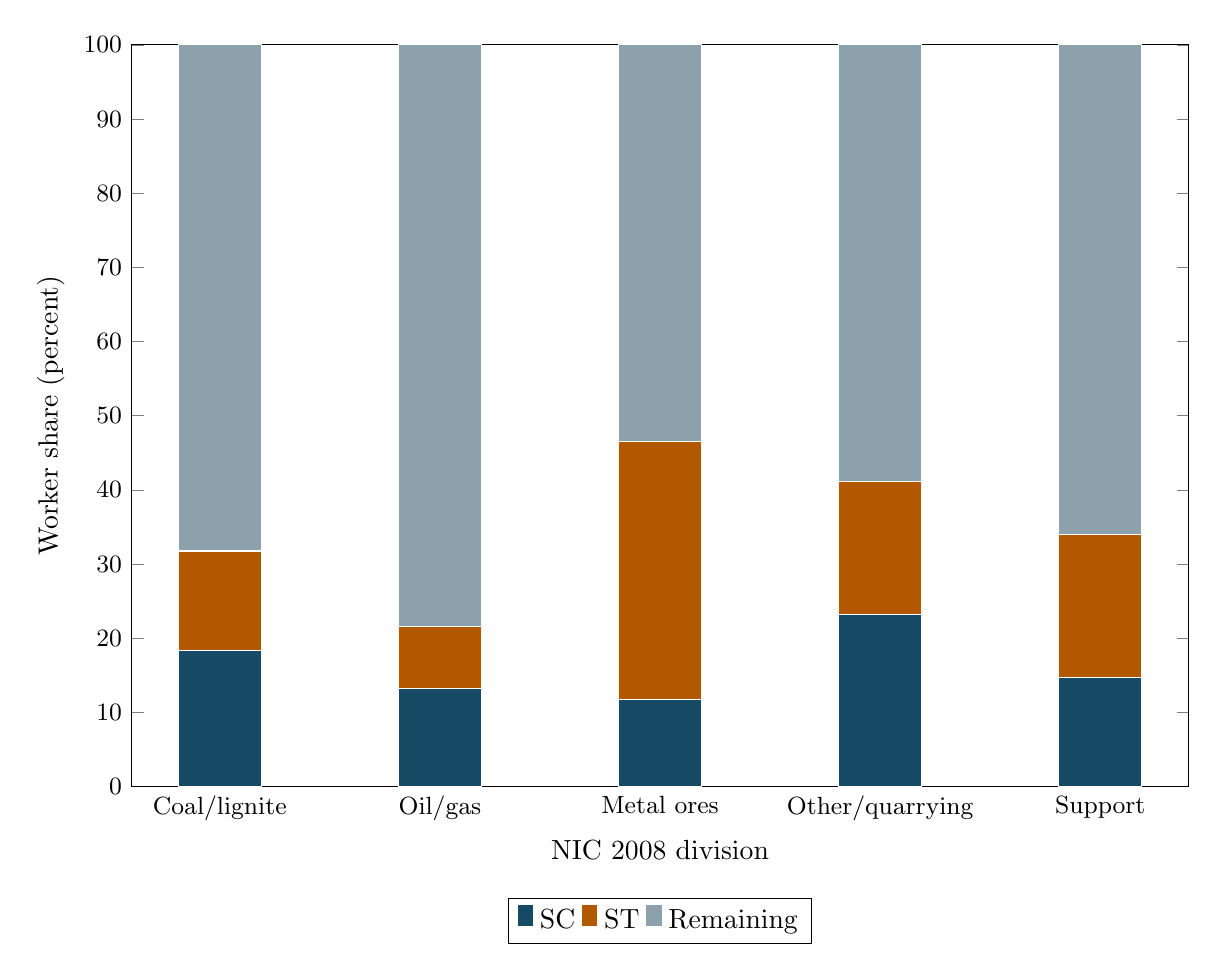
\begin{tikzpicture}
\begin{axis}[width=15cm,height=11cm,ybar stacked,bar width=30pt,ymin=0,ymax=100,xtick={0,1,2,3,4},xticklabels={Coal/lignite,Oil/gas,Metal ores,Other/quarrying,Support},ylabel={Worker share (percent)},xlabel={NIC 2008 division},legend style={at={(0.5,-0.15)},anchor=north,legend columns=3},tick label style={font=\small}]
\addplot[fill=navy,draw=white] coordinates {(0,18.29238) (1,13.22423) (2,11.72302) (3,23.14495) (4,14.67866)};
\addlegendentry{SC}
\addplot[fill=orange!70!black,draw=white] coordinates {(0,13.46477) (1,8.305303) (2,34.8279) (3,18.01872) (4,19.24568)};
\addlegendentry{ST}
\addplot[fill=muted,draw=white] coordinates {(0,68.24285) (1,78.47046) (2,53.44908) (3,58.83633) (4,66.07566)};
\addlegendentry{Remaining}

\end{axis}
\end{tikzpicture}}

\caption{National SC/\allowbreak{}ST mining worker composition, main plus marginal, by NIC divisions 05-09. Source: Census 2011 B18, B18SC and B18ST. Remaining contains OBC and other workers. This directly classifies worker identity, unlike EC employment classified by owner identity.}\end{figure}\clearpage
\clearpage\begin{figure}[p]\centering
\resizebox{\linewidth}{!}{%
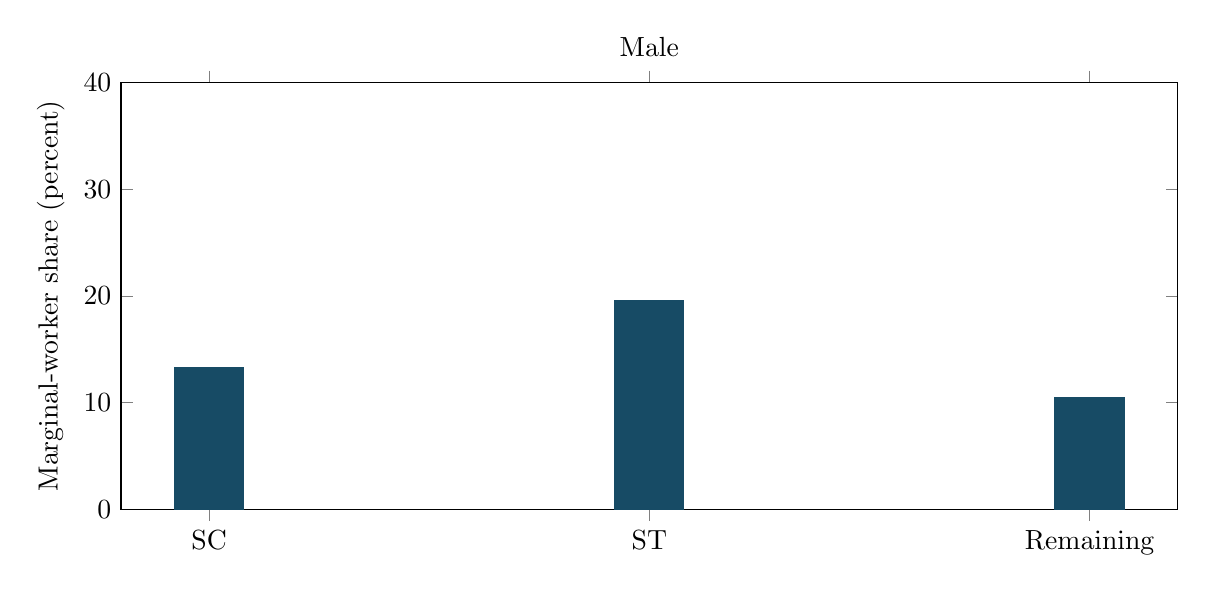
\begin{tikzpicture}
\begin{axis}[width=15cm,height=7cm,ybar,bar width=25pt,xtick={0,1,2},xticklabels={SC,ST,Remaining},ymin=0,ymax=40,ylabel={Marginal-worker share (percent)},title={Male}]
\addplot[navy,fill=navy] coordinates {(0,13.25275) (1,19.55057) (2,10.45077)};
\end{axis}
\end{tikzpicture}}

\par\vspace{0.4cm}
\resizebox{\linewidth}{!}{%
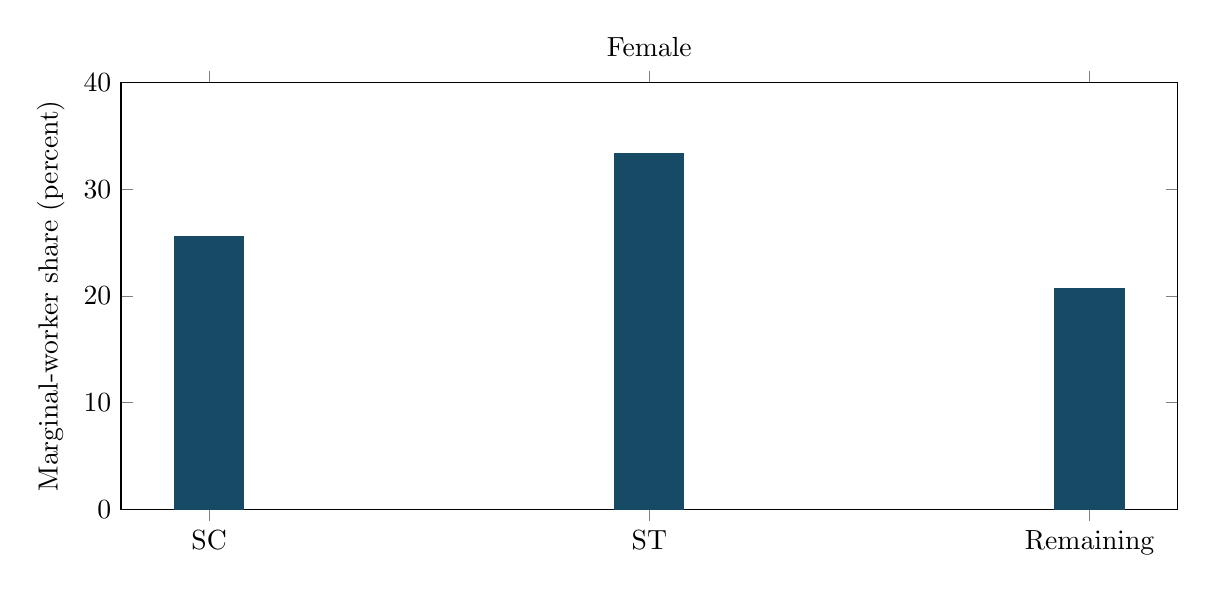
\begin{tikzpicture}
\begin{axis}[width=15cm,height=7cm,ybar,bar width=25pt,xtick={0,1,2},xticklabels={SC,ST,Remaining},ymin=0,ymax=40,ylabel={Marginal-worker share (percent)},title={Female}]
\addplot[navy,fill=navy] coordinates {(0,25.56459) (1,33.32071) (2,20.64947)};
\end{axis}
\end{tikzpicture}}

\par\vspace{0.4cm}
\caption{Sex-specific marginal-worker shares across NIC 05-09, Census 2011. Marginal denotes work for less than six months during the preceding reference year. It is not a measure of contractor employment, informality or a particular occupation.}\end{figure}\clearpage
\clearpage\begin{figure}[p]\centering
\resizebox{\linewidth}{!}{%
\begin{tikzpicture}
\begin{axis}[width=15cm,height=11cm,ytick={0,1,2,3},yticklabels={W1 group only,W2 sex + residence,W3 + state + division,W4 joint strata},yticklabel style={text width=4cm,align=right},y dir=reverse,xlabel={Contrast vs Remaining (percentage points)},legend style={at={(0.5,-0.15)},anchor=north,legend columns=2},tick label style={font=\small}]
\addplot[gray,dashed,mark=none,forget plot] coordinates {(0,-0.5)(0,3.5)};\addplot+[only marks,mark=*,color=navy,error bars/.cd,x dir=both,x explicit] coordinates {(3.83325,-0.1) +- (2.296031,0) (2.467763,0.9) +- (1.67724,0) (1.890553,1.9) +- (1.540951,0) (1.493233,2.9) +- (1.956763,0)};
\addlegendentry{SC}
\addplot+[only marks,mark=*,color=orange!70!black,error bars/.cd,x dir=both,x explicit] coordinates {(10.98901,0.1) +- (2.469842,0) (7.575182,1.1) +- (2.127297,0) (6.228437,2.1) +- (1.068707,0) (5.083905,3.1) +- (1.501008,0)};
\addlegendentry{ST}

\end{axis}
\end{tikzpicture}}

\caption{Observed aggregate duration differences before and after controls. Employment-weighted WLS on 1,275 cells. W4 absorbs state-by-division-by-sex-by-residence strata. Intervals cluster at 35 historical states and are model-based, not Census enumeration errors or causal caste effects. Missing age, education and occupation controls remain relevant.}\end{figure}\clearpage
\clearpage\begin{figure}[p]\centering
\resizebox{\linewidth}{!}{%
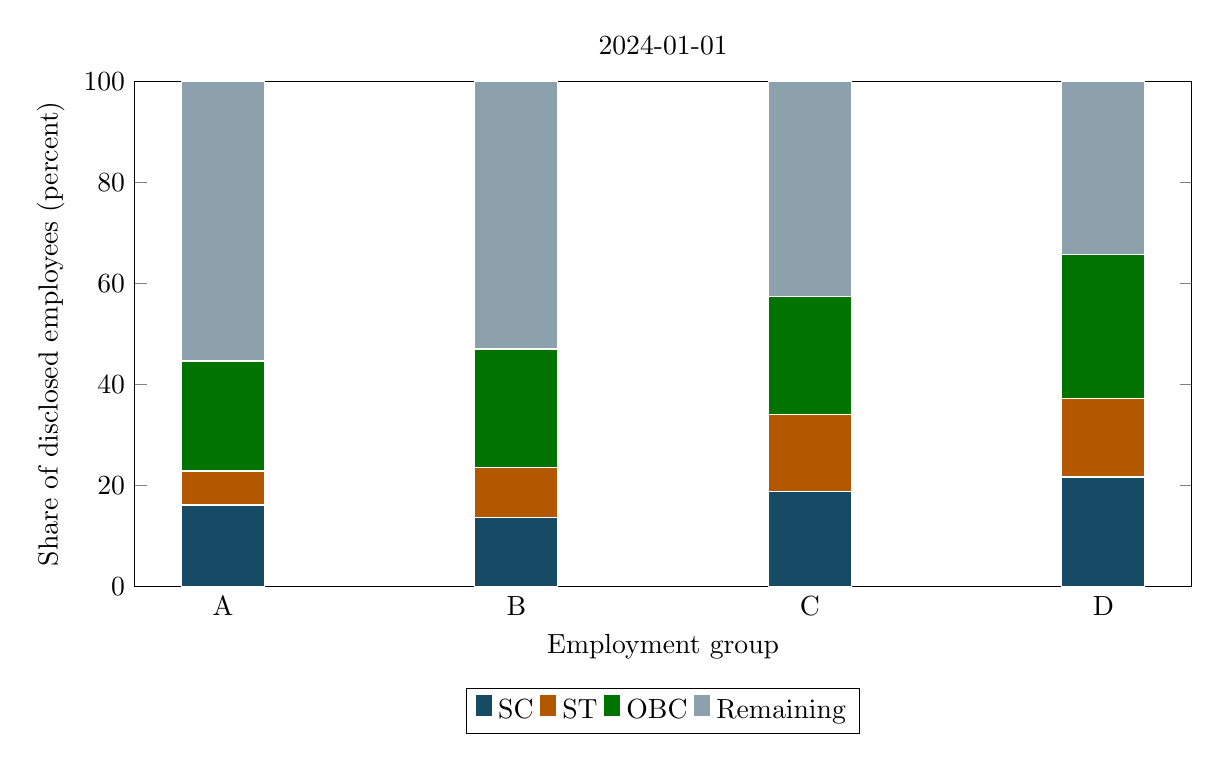
\begin{tikzpicture}
\begin{axis}[width=15cm,height=8cm,ybar stacked,bar width=30pt,ymin=0,ymax=100,xtick={0,1,2,3},xticklabels={A,B,C,D},ylabel={Share of disclosed employees (percent)},title={2024-01-01},xlabel={Employment group},legend style={at={(0.5,-0.2)},anchor=north,legend columns=4}]
\addplot[fill=navy,draw=white] coordinates {(0,16.13446) (1,13.61804) (2,18.77131) (3,21.67223)};
\addlegendentry{SC}
\addplot[fill=orange!70!black,draw=white] coordinates {(0,6.716756) (1,9.940127) (2,15.17628) (3,15.45726)};
\addlegendentry{ST}
\addplot[fill=green!45!black,draw=white] coordinates {(0,21.76954) (1,23.42986) (2,23.50698) (3,28.49453)};
\addlegendentry{OBC}
\addplot[fill=muted,draw=white] coordinates {(0,55.37923) (1,53.01197) (2,42.54543) (3,34.37599)};
\addlegendentry{Remaining}

\end{axis}
\end{tikzpicture}}

\par\vspace{1cm}
\resizebox{\linewidth}{!}{%
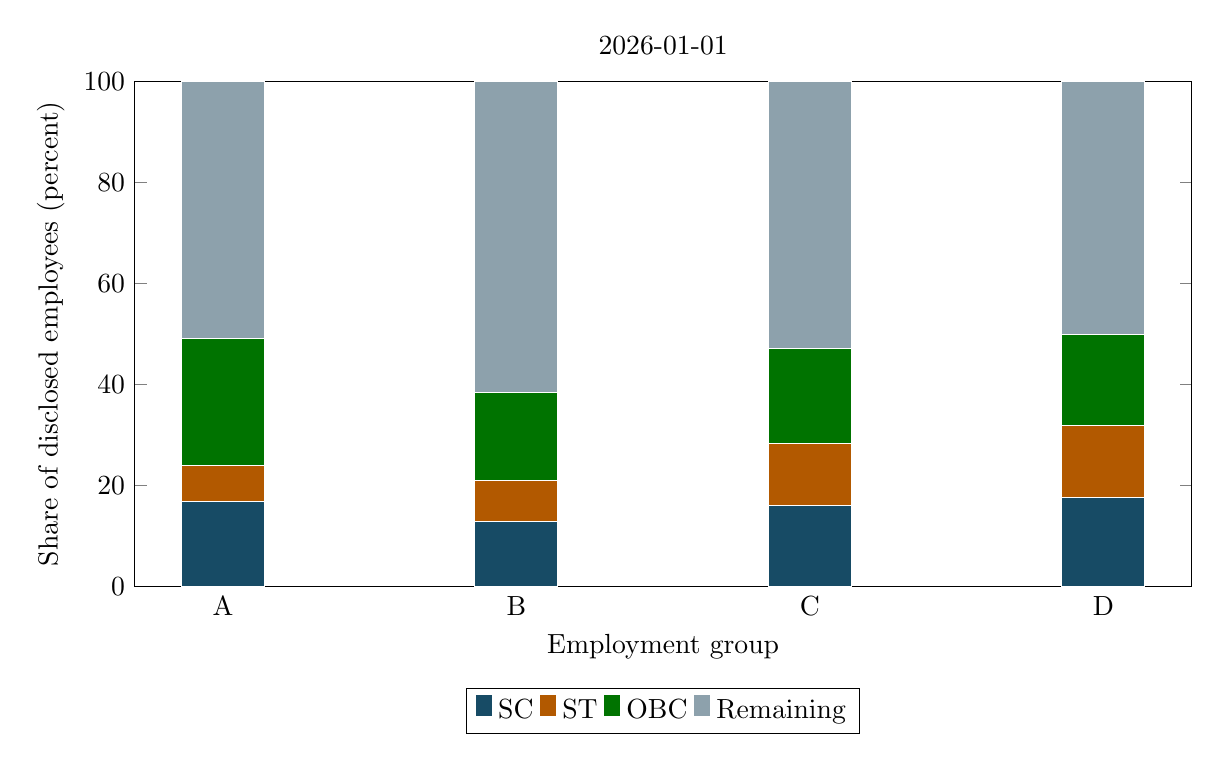
\begin{tikzpicture}
\begin{axis}[width=15cm,height=8cm,ybar stacked,bar width=30pt,ymin=0,ymax=100,xtick={0,1,2,3},xticklabels={A,B,C,D},ylabel={Share of disclosed employees (percent)},title={2026-01-01},xlabel={Employment group},legend style={at={(0.5,-0.2)},anchor=north,legend columns=4}]
\addplot[fill=navy,draw=white] coordinates {(0,16.73771) (1,12.78463) (2,15.95503) (3,17.64113)};
\addlegendentry{SC}
\addplot[fill=orange!70!black,draw=white] coordinates {(0,7.186626) (1,8.238457) (2,12.34691) (3,14.20696)};
\addlegendentry{ST}
\addplot[fill=green!45!black,draw=white] coordinates {(0,25.0766) (1,17.38615) (2,18.8581) (3,17.95311)};
\addlegendentry{OBC}
\addplot[fill=muted,draw=white] coordinates {(0,50.99907) (1,61.59077) (2,52.83996) (3,50.1988)};
\addlegendentry{Remaining}

\end{axis}
\end{tikzpicture}}

\par\vspace{1cm}
\caption{Coal India corporate employee composition by administrative employment group. Source: Coal Ministry annual reports 2023-24 and 2025-26, chapter 16, PDF pages 5 and 4. The 2026 residual contains EWS employees. Snapshots do not identify recruitment probabilities or the reasons for changes in employee stocks.}\end{figure}\clearpage
\clearpage\begin{figure}[p]\centering
\resizebox{\linewidth}{!}{%
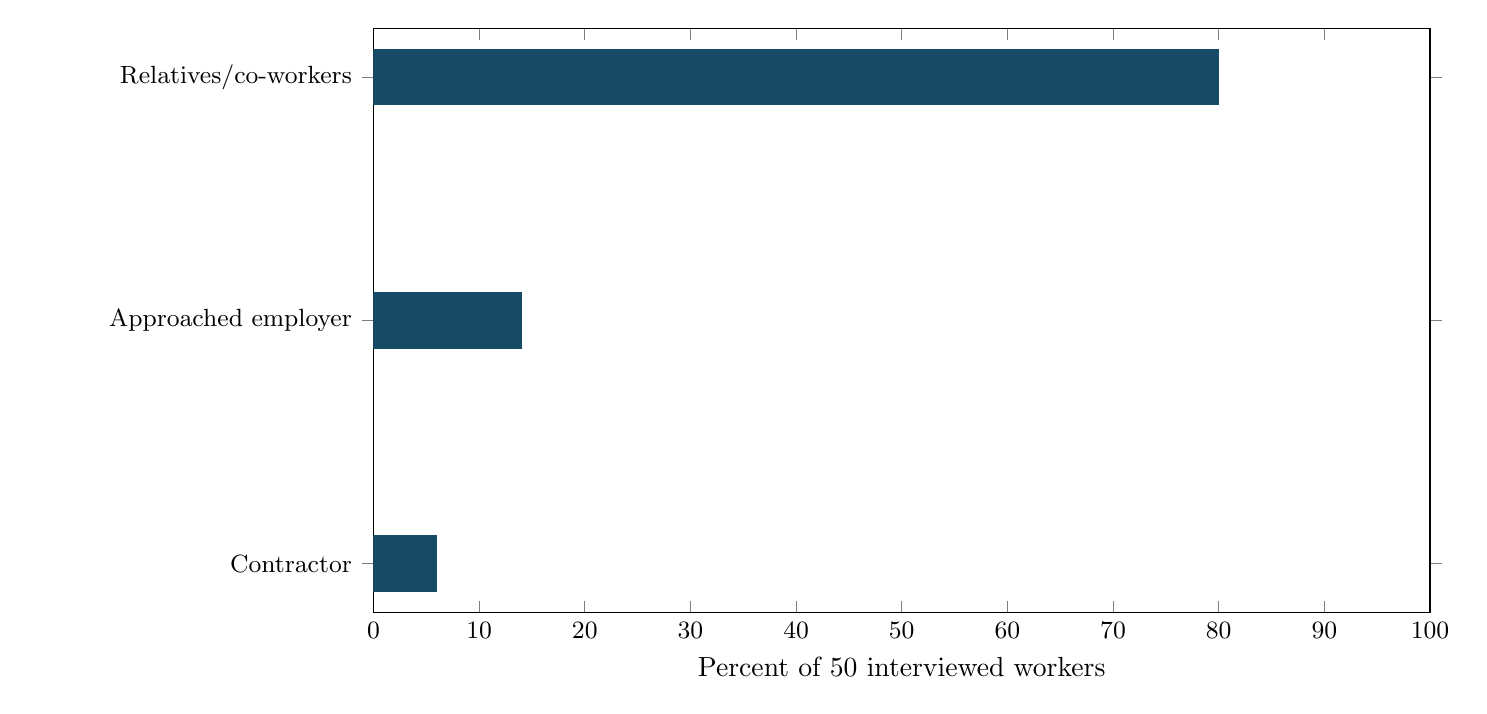
\begin{tikzpicture}
\begin{axis}[width=15cm,height=9cm,xbar,xmin=0,xmax=100,ytick={0,1,2},yticklabels={Relatives/co-workers,Approached employer,Contractor},yticklabel style={text width=4cm,align=right},y dir=reverse,xlabel={Percent of 50 interviewed workers},bar width=20pt,tick label style={font=\small}]
\addplot[fill=navy,draw=navy] coordinates {(80,0) (14,1) (6,2)};
\end{axis}
\end{tikzpicture}}

\caption{Reported Makrana job-entry routes, Arisa/\allowbreak{}CLRA 2024, PDF page 29. Published counts are seven direct approaches and three contractor recruits; 40 referral entrants are derived from the published 80 percent of N=50. This is a local supply-chain sample and referrals do not establish shared-caste relationships.}\end{figure}\clearpage
\clearpage\begin{figure}[p]\centering
\resizebox{\linewidth}{!}{%
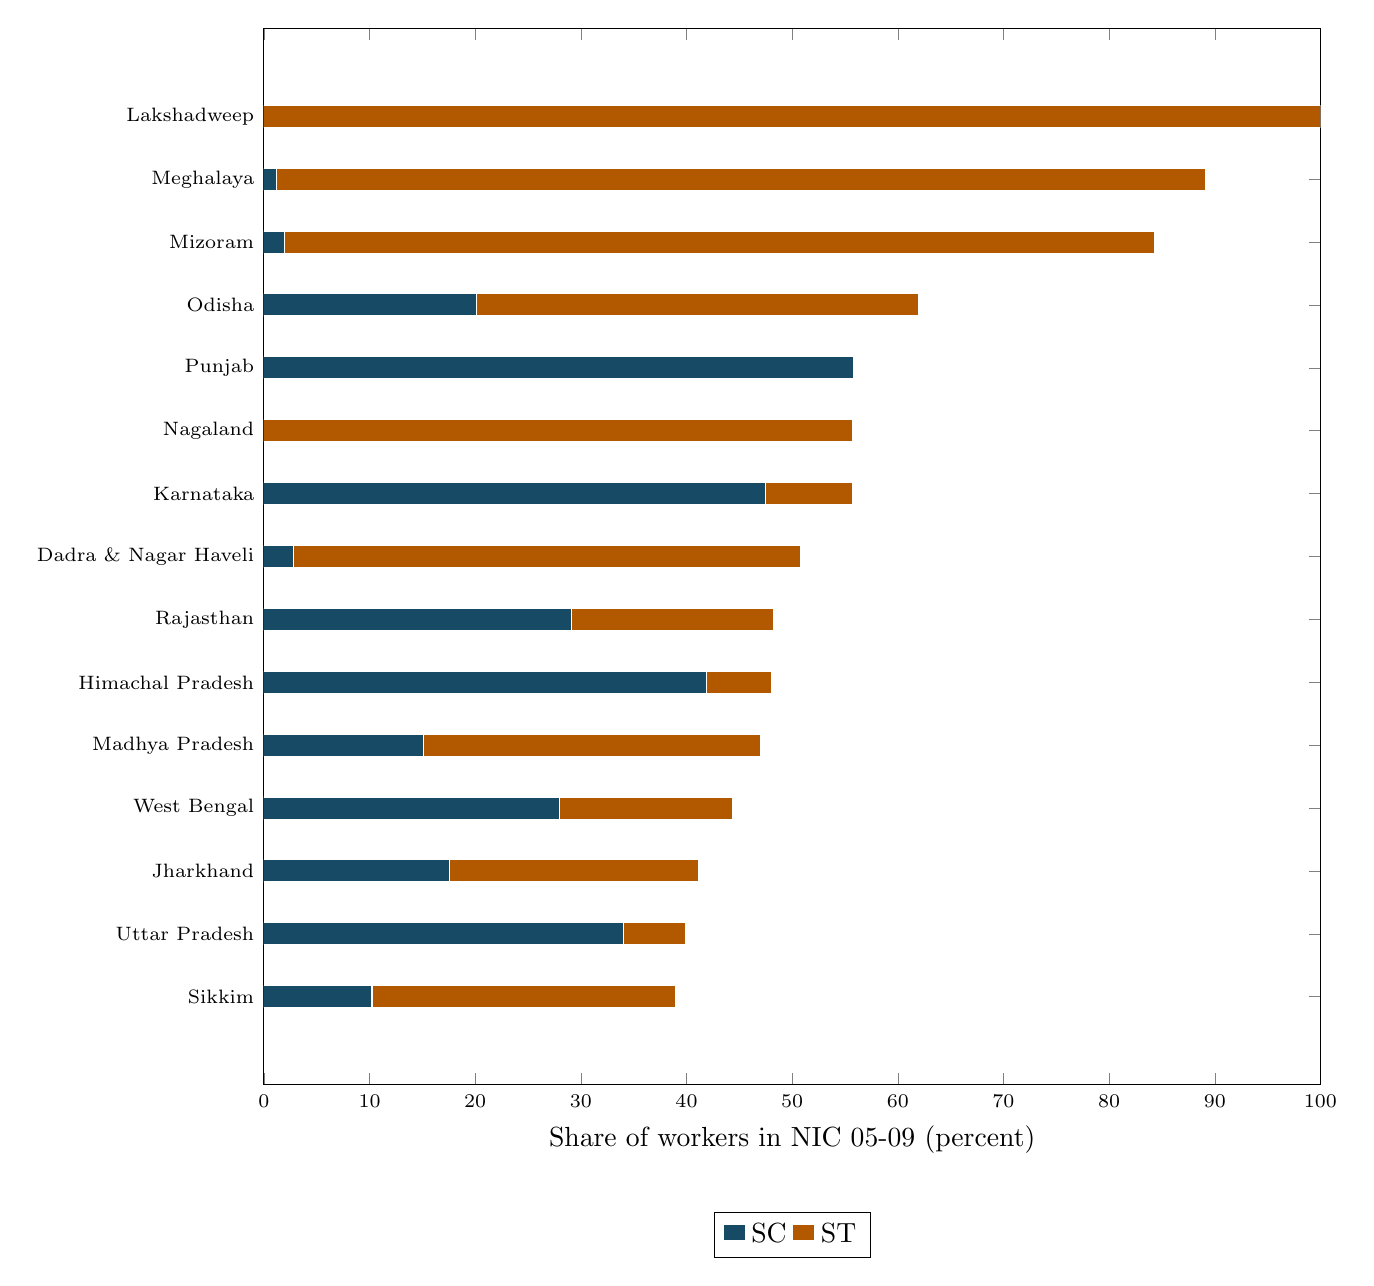
\begin{tikzpicture}
\begin{axis}[width=15cm,height=15cm,xbar stacked,xmin=0,xmax=100,ytick={0,1,2,3,4,5,6,7,8,9,10,11,12,13,14},yticklabels={{Sikkim},{Uttar Pradesh},{Jharkhand},{West Bengal},{Madhya Pradesh},{Himachal Pradesh},{Rajasthan},{Dadra \& Nagar Haveli},{Karnataka},{Nagaland},{Punjab},{Odisha},{Mizoram},{Meghalaya},{Lakshadweep}},tick label style={font=\scriptsize},xlabel={Share of workers in NIC 05-09 (percent)},bar width=8pt,legend style={at={(0.5,-0.12)},anchor=north,legend columns=2}]
\addplot[fill=navy,draw=white] coordinates {(10.23392,0) (34.06162,1) (17.60081,2) (27.96329,3) (15.13101,4) (41.88063,5) (29.0878,6) (2.771363,7) (47.50018,8) (0,9) (55.81505,10) (20.16398,11) (1.936872,12) (1.198271,13) (0,14)};
\addlegendentry{SC}
\addplot[fill=orange!70!black,draw=white] coordinates {(28.75244,0) (5.870758,1) (23.54432,2) (16.35169,3) (31.9095,4) (6.202067,5) (19.14473,6) (48.03695,7) (8.203208,8) (55.73394,9) (0,10) (41.82127,11) (82.35294,12) (87.91886,13) (100,14)};
\addlegendentry{ST}

\end{axis}
\end{tikzpicture}}

\caption{Fifteen highest SC plus ST worker shares, Census 2011 historical state/\allowbreak{}UT geography. Some regions have very small workforces; the full count table should accompany comparisons. These are workforce composition shares, not mining participation rates among the regional SC/\allowbreak{}ST population.}\end{figure}\clearpage
\clearpage\begin{figure}[p]\centering
\resizebox{\linewidth}{!}{%
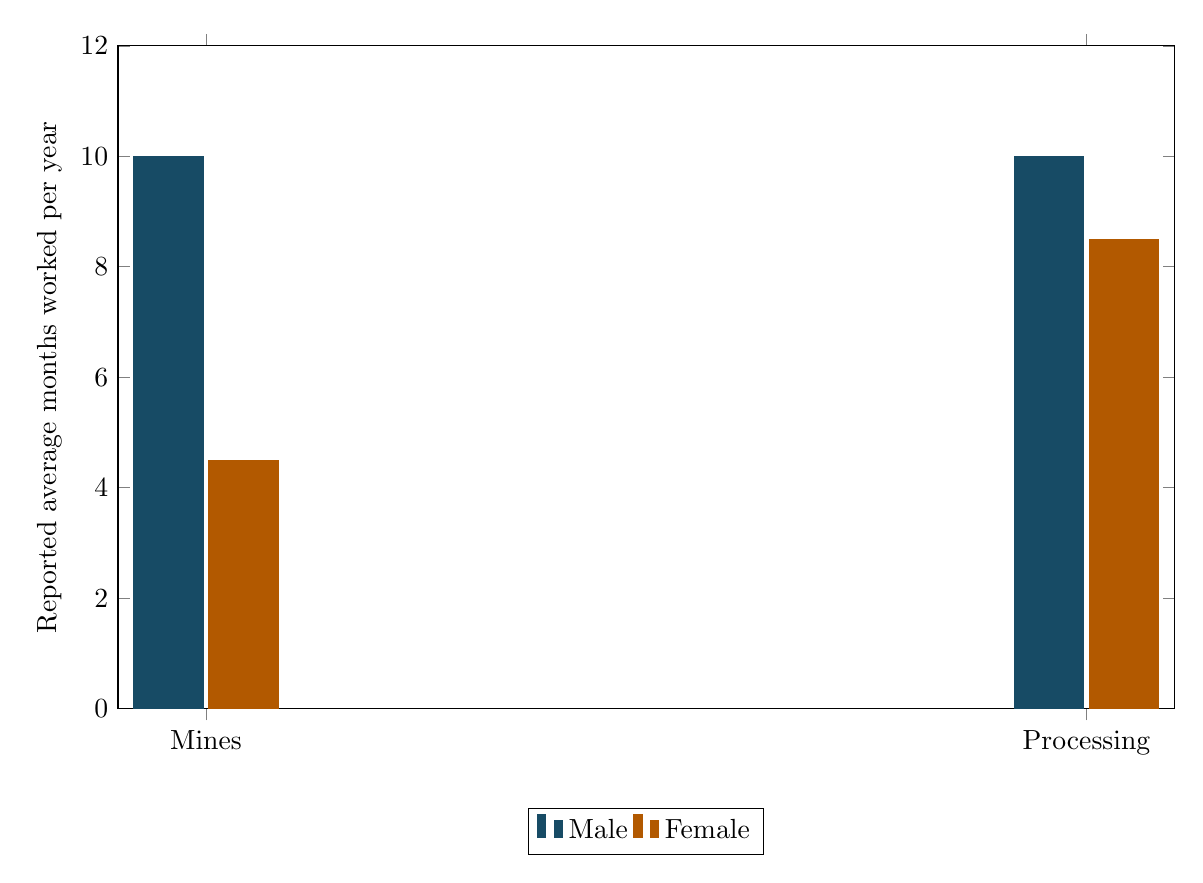
\begin{tikzpicture}
\begin{axis}[width=15cm,height=10cm,ybar,bar width=25pt,ymin=0,ymax=12,xtick={0,1},xticklabels={Mines,Processing},ylabel={Reported average months worked per year},legend style={at={(0.5,-0.15)},anchor=north,legend columns=2}]
\addplot[fill=navy,draw=navy] coordinates {(0,10) (1,10)};
\addlegendentry{Male}
\addplot[fill=orange!70!black,draw=orange!70!black] coordinates {(0,4.5) (1,8.5)};
\addlegendentry{Female}

\end{axis}
\end{tikzpicture}}

\caption{Published local working-year averages by sex and stone supply-chain stage. ILO Rajasthan study 2021, PDF page 59. These unadjusted averages do not control for occupation, caste or worker characteristics and should not be read as a causal gender effect.}\end{figure}\clearpage
\chapter{Worker statistics and controlled-result tables}
All national and state values are derived from actual B18 cells. Census categories and company reservation classifications are kept separate. Model coefficients use percentage points. Full-precision values, source coordinates and all fitted coefficients are archived in CSV files.
\begingroup\footnotesize\setlength{\tabcolsep}{4pt}
\begin{longtable}{lrrrrr}
\caption{Census 2011 national mining workforce, NIC 05-09}\\\toprule
Group & Main & Marginal & All workers & Worker \% & Marginal \% \\\midrule\endfirsthead
\multicolumn{6}{l}{\textit{Continued from previous page}}\\\toprule
Group & Main & Marginal & All workers & Worker \% & Marginal \% \\\midrule\endhead
\midrule\multicolumn{6}{r}{\textit{Continued on next page}}\\\endfoot\bottomrule\endlastfoot
SC & 371,016 & 68,503 & 439,519 & 20.87 & 15.59 \\
ST & 281,799 & 82,950 & 364,749 & 17.32 & 22.74 \\
Remaining & 1,148,511 & 152,957 & 1,301,468 & 61.81 & 11.75 \\
\end{longtable}\endgroup
\begingroup\footnotesize\setlength{\tabcolsep}{4pt}
\begin{longtable}{l>{\raggedright\arraybackslash}p{4.5cm}lrrr}
\caption{National workforce composition by mining division}\\\toprule
NIC & Division & Group & Workers & Worker \% & Marginal \% \\\midrule\endfirsthead
\multicolumn{6}{l}{\textit{Continued from previous page}}\\\toprule
NIC & Division & Group & Workers & Worker \% & Marginal \% \\\midrule\endhead
\midrule\multicolumn{6}{r}{\textit{Continued on next page}}\\\endfoot\bottomrule\endlastfoot
05 & Coal and lignite & Remaining & 398,831 & 68.24 & 4.46 \\
05 & Coal and lignite & SC & 106,906 & 18.29 & 6.04 \\
05 & Coal and lignite & ST & 78,692 & 13.46 & 13.76 \\
06 & Oil and natural gas & Remaining & 41,525 & 78.47 & 7.02 \\
06 & Oil and natural gas & SC & 6,998 & 13.22 & 13.79 \\
06 & Oil and natural gas & ST & 4,395 & 8.31 & 16.68 \\
07 & Metal ores & Remaining & 52,952 & 53.45 & 9.09 \\
07 & Metal ores & SC & 11,614 & 11.72 & 11.19 \\
07 & Metal ores & ST & 34,504 & 34.83 & 17.88 \\
08 & Other mining /\allowbreak{} quarrying & Remaining & 785,315 & 58.84 & 15.97 \\
08 & Other mining /\allowbreak{} quarrying & SC & 308,926 & 23.14 & 19.08 \\
08 & Other mining /\allowbreak{} quarrying & ST & 240,504 & 18.02 & 26.56 \\
09 & Mining support & Remaining & 22,845 & 66.08 & 8.66 \\
09 & Mining support & SC & 5,075 & 14.68 & 16.33 \\
09 & Mining support & ST & 6,654 & 19.25 & 20.26 \\
\end{longtable}\endgroup
\begingroup\footnotesize\setlength{\tabcolsep}{4pt}
\begin{longtable}{>{\raggedright\arraybackslash}p{4cm}rrrrrr}
\caption{All 35 historical regions: workforce counts and social composition}\\\toprule
Region & Workers & SC count & ST count & SC \% & ST \% & Marg. \% \\\midrule\endfirsthead
\multicolumn{7}{l}{\textit{Continued from previous page}}\\\toprule
Region & Workers & SC count & ST count & SC \% & ST \% & Marg. \% \\\midrule\endhead
\midrule\multicolumn{7}{r}{\textit{Continued on next page}}\\\endfoot\bottomrule\endlastfoot
Jammu \& Kashmir & 6,384 & 309 & 217 & 4.84 & 3.40 & 25.44 \\
Himachal Pradesh & 2,999 & 1,256 & 186 & 41.88 & 6.20 & 25.44 \\
Punjab & 4,239 & 2,366 & 0 & 55.82 & 0.00 & 10.43 \\
Chandigarh & 89 & 6 & 0 & 6.74 & 0.00 & 0.00 \\
Uttarakhand & 8,091 & 1,387 & 276 & 17.14 & 3.41 & 32.75 \\
Haryana & 9,392 & 1,802 & 0 & 19.19 & 0.00 & 19.73 \\
Nct Of Delhi & 777 & 136 & 0 & 17.50 & 0.00 & 3.09 \\
Rajasthan & 235,903 & 68,619 & 45,163 & 29.09 & 19.14 & 16.38 \\
Uttar Pradesh & 65,954 & 22,465 & 3,872 & 34.06 & 5.87 & 23.23 \\
Bihar & 27,736 & 8,478 & 964 & 30.57 & 3.48 & 23.33 \\
Sikkim & 1,026 & 105 & 295 & 10.23 & 28.75 & 18.13 \\
Arunachal Pradesh & 1,038 & 0 & 243 & 0.00 & 23.41 & 11.66 \\
Nagaland & 3,052 & 0 & 1,701 & 0.00 & 55.73 & 40.20 \\
Manipur & 1,858 & 47 & 134 & 2.53 & 7.21 & 17.98 \\
Mizoram & 1,394 & 27 & 1,148 & 1.94 & 82.35 & 16.57 \\
Tripura & 2,707 & 308 & 392 & 11.38 & 14.48 & 18.06 \\
Meghalaya & 23,367 & 280 & 20,544 & 1.20 & 87.92 & 29.66 \\
Assam & 75,909 & 4,578 & 7,291 & 6.03 & 9.60 & 19.31 \\
West Bengal & 155,250 & 43,413 & 25,386 & 27.96 & 16.35 & 14.68 \\
Jharkhand & 286,430 & 50,414 & 67,438 & 17.60 & 23.54 & 13.11 \\
Odisha & 166,609 & 33,595 & 69,678 & 20.16 & 41.82 & 21.55 \\
Chhattisgarh & 78,687 & 10,076 & 17,974 & 12.81 & 22.84 & 5.14 \\
Madhya Pradesh & 157,392 & 23,815 & 50,223 & 15.13 & 31.91 & 13.71 \\
Gujarat & 55,447 & 4,275 & 7,387 & 7.71 & 13.32 & 11.44 \\
Daman \& Diu & 451 & 17 & 84 & 3.77 & 18.63 & 2.00 \\
Dadra \& Nagar Haveli & 433 & 12 & 208 & 2.77 & 48.04 & 16.63 \\
Maharashtra & 126,535 & 16,055 & 17,257 & 12.69 & 13.64 & 9.96 \\
Andhra Pradesh & 223,499 & 37,379 & 9,354 & 16.72 & 4.19 & 8.77 \\
Karnataka & 141,530 & 67,227 & 11,610 & 47.50 & 8.20 & 14.03 \\
Goa & 18,321 & 261 & 2,178 & 1.42 & 11.89 & 14.88 \\
Lakshadweep & 3 & 0 & 3 & 0.00 & 100.00 & 33.33 \\
Kerala & 77,142 & 14,371 & 2,084 & 18.63 & 2.70 & 18.43 \\
Tamil Nadu & 144,416 & 26,314 & 1,456 & 18.22 & 1.01 & 10.37 \\
Puducherry & 822 & 126 & 0 & 15.33 & 0.00 & 6.08 \\
Andaman \& Nicobar Islands & 854 & 0 & 3 & 0.00 & 0.35 & 12.41 \\
\end{longtable}\endgroup
\begingroup\footnotesize\setlength{\tabcolsep}{4pt}
\begin{longtable}{lrrrrr}
\caption{National worker sex and duration cells}\\\toprule
Sex & Group & Main & Marginal & Workers & Marginal \% \\\midrule\endfirsthead
\multicolumn{6}{l}{\textit{Continued from previous page}}\\\toprule
Sex & Group & Main & Marginal & Workers & Marginal \% \\\midrule\endhead
\midrule\multicolumn{6}{r}{\textit{Continued on next page}}\\\endfoot\bottomrule\endlastfoot
Female & Remaining & 131,829 & 34,306 & 166,135 & 20.65 \\
Female & SC & 61,998 & 21,293 & 83,291 & 25.56 \\
Female & ST & 56,362 & 28,165 & 84,527 & 33.32 \\
Male & Remaining & 1,016,682 & 118,651 & 1,135,333 & 10.45 \\
Male & SC & 309,018 & 47,210 & 356,228 & 13.25 \\
Male & ST & 225,437 & 54,785 & 280,222 & 19.55 \\
\end{longtable}\endgroup
\begingroup\footnotesize\setlength{\tabcolsep}{4pt}
\begin{longtable}{l>{\raggedright\arraybackslash}p{5cm}rrrrr}
\caption{Worker-cell specifications: weighting and control sets}\\\toprule
Model & Controls & Cells & States & Weight sum & Rank & R sq. \\\midrule\endfirsthead
\multicolumn{7}{l}{\textit{Continued from previous page}}\\\toprule
Model & Controls & Cells & States & Weight sum & Rank & R sq. \\\midrule\endhead
\midrule\multicolumn{7}{r}{\textit{Continued on next page}}\\\endfoot\bottomrule\endlastfoot
W1 & Group only & 1275 & 35 & 2,105,736 & 3 & 0.1599 \\
W2 & Sex + rural/\allowbreak{}urban & 1275 & 35 & 2,105,736 & 5 & 0.5201 \\
W3 & Sex + area + state + division & 1275 & 35 & 2,105,736 & 43 & 0.7856 \\
W4 & State-division-sex-area strata & 1275 & 35 & 2,105,736 & 552 & 0.9349 \\
\end{longtable}\endgroup
\begingroup\footnotesize\setlength{\tabcolsep}{4pt}
\begin{longtable}{lrrrrrr}
\caption{Unadjusted and controlled SC/\allowbreak{}ST duration contrasts versus Remaining}\\\toprule
Model & Group & Beta pp & Cluster SE & 95\% low & 95\% high & Model p \\\midrule\endfirsthead
\multicolumn{7}{l}{\textit{Continued from previous page}}\\\toprule
Model & Group & Beta pp & Cluster SE & 95\% low & 95\% high & Model p \\\midrule\endhead
\midrule\multicolumn{7}{r}{\textit{Continued on next page}}\\\endfoot\bottomrule\endlastfoot
W1 & SC & 3.833 & 1.130 & 1.537 & 6.129 & 0.0018 \\
W1 & ST & 10.989 & 1.215 & 8.519 & 13.459 & 0.0000 \\
W2 & SC & 2.468 & 0.825 & 0.791 & 4.145 & 0.0052 \\
W2 & ST & 7.575 & 1.047 & 5.448 & 9.702 & 0.0000 \\
W3 & SC & 1.891 & 0.758 & 0.350 & 3.432 & 0.0177 \\
W3 & ST & 6.228 & 0.526 & 5.160 & 7.297 & 0.0000 \\
W4 & SC & 1.493 & 0.963 & -0.464 & 3.450 & 0.1302 \\
W4 & ST & 5.084 & 0.739 & 3.583 & 6.585 & 0.0000 \\
\end{longtable}\endgroup
W1 group-only; W2 sex/residence; W3 additionally state and division effects; W4 joint state-division-sex-residence strata. All models have 1,275 nonempty aggregate cells and 35 state clusters. Point estimates describe the acquired cells; p-values are exploratory model summaries. They are not part of the earlier 18-coefficient EC multiple-testing family and are not used for a causal claim.
\begingroup\footnotesize\setlength{\tabcolsep}{4pt}
\begin{longtable}{l>{\raggedright\arraybackslash}p{6cm}rrrr}
\caption{All coefficients including controls in W1-W3}\\\toprule
Model & Term & Beta pp & Cluster SE & 95\% low & 95\% high \\\midrule\endfirsthead
\multicolumn{6}{l}{\textit{Continued from previous page}}\\\toprule
Model & Term & Beta pp & Cluster SE & 95\% low & 95\% high \\\midrule\endhead
\midrule\multicolumn{6}{r}{\textit{Continued on next page}}\\\endfoot\bottomrule\endlastfoot
W1 & Intercept & 11.753 & 0.936 & 9.851 & 13.654 \\
W1 & C(group)[T.SC] & 3.833 & 1.130 & 1.537 & 6.129 \\
W1 & C(group)[T.ST] & 10.989 & 1.215 & 8.519 & 13.459 \\
W2 & Intercept & 24.968 & 2.093 & 20.714 & 29.221 \\
W2 & C(group)[T.SC] & 2.468 & 0.825 & 0.791 & 4.145 \\
W2 & C(group)[T.ST] & 7.575 & 1.047 & 5.448 & 9.702 \\
W2 & C(sex)[T.Male] & -10.559 & 1.451 & -13.508 & -7.610 \\
W2 & C(area)[T.Urban] & -9.491 & 1.176 & -11.880 & -7.101 \\
W3 & Intercept & 28.525 & 1.739 & 24.991 & 32.059 \\
W3 & C(group)[T.SC] & 1.891 & 0.758 & 0.350 & 3.432 \\
W3 & C(group)[T.ST] & 6.228 & 0.526 & 5.160 & 7.297 \\
W3 & C(sex)[T.Male] & -10.111 & 1.331 & -12.816 & -7.406 \\
W3 & C(area)[T.Urban] & -5.504 & 0.889 & -7.311 & -3.697 \\
W3 & C(state\_code)[T.02] & -2.867 & 0.480 & -3.843 & -1.891 \\
W3 & C(state\_code)[T.03] & -16.750 & 0.462 & -17.689 & -15.810 \\
W3 & C(state\_code)[T.04] & -20.420 & 0.655 & -21.750 & -19.090 \\
W3 & C(state\_code)[T.05] & 6.286 & 0.181 & 5.919 & 6.654 \\
W3 & C(state\_code)[T.06] & -6.897 & 0.219 & -7.342 & -6.453 \\
W3 & C(state\_code)[T.07] & -15.449 & 1.093 & -17.671 & -13.228 \\
W3 & C(state\_code)[T.08] & -12.533 & 0.371 & -13.288 & -11.778 \\
W3 & C(state\_code)[T.09] & -3.505 & 0.309 & -4.132 & -2.878 \\
W3 & C(state\_code)[T.10] & -2.416 & 0.340 & -3.107 & -1.725 \\
W3 & C(state\_code)[T.11] & -13.550 & 0.635 & -14.841 & -12.259 \\
W3 & C(state\_code)[T.12] & -16.212 & 0.510 & -17.247 & -15.176 \\
W3 & C(state\_code)[T.13] & 12.940 & 0.378 & 12.172 & 13.708 \\
W3 & C(state\_code)[T.14] & -13.406 & 0.770 & -14.972 & -11.841 \\
W3 & C(state\_code)[T.15] & -11.923 & 0.791 & -13.531 & -10.315 \\
W3 & C(state\_code)[T.16] & -9.294 & 1.115 & -11.560 & -7.028 \\
W3 & C(state\_code)[T.17] & 1.728 & 0.881 & -0.063 & 3.518 \\
W3 & C(state\_code)[T.18] & -4.967 & 0.756 & -6.503 & -3.431 \\
W3 & C(state\_code)[T.19] & -8.440 & 0.415 & -9.284 & -7.596 \\
W3 & C(state\_code)[T.20] & -10.086 & 0.548 & -11.200 & -8.973 \\
W3 & C(state\_code)[T.21] & -6.813 & 0.375 & -7.574 & -6.051 \\
W3 & C(state\_code)[T.22] & -14.106 & 0.908 & -15.950 & -12.261 \\
W3 & C(state\_code)[T.23] & -10.968 & 0.439 & -11.860 & -10.076 \\
W3 & C(state\_code)[T.24] & -15.007 & 0.527 & -16.077 & -13.937 \\
W3 & C(state\_code)[T.25] & -22.960 & 0.424 & -23.822 & -22.097 \\
W3 & C(state\_code)[T.26] & -11.549 & 0.316 & -12.190 & -10.907 \\
W3 & C(state\_code)[T.27] & -13.885 & 0.337 & -14.571 & -13.199 \\
W3 & C(state\_code)[T.28] & -15.900 & 0.327 & -16.564 & -15.235 \\
W3 & C(state\_code)[T.29] & -14.799 & 0.465 & -15.745 & -13.854 \\
W3 & C(state\_code)[T.30] & -8.291 & 0.515 & -9.338 & -7.245 \\
W3 & C(state\_code)[T.31] & -1.631 & 0.794 & -3.244 & -0.017 \\
W3 & C(state\_code)[T.32] & -8.172 & 0.163 & -8.504 & -7.840 \\
W3 & C(state\_code)[T.33] & -15.271 & 0.254 & -15.788 & -14.755 \\
W3 & C(state\_code)[T.34] & -13.878 & 1.440 & -16.804 & -10.952 \\
W3 & C(state\_code)[T.35] & -14.410 & 0.199 & -14.813 & -14.006 \\
W3 & C(division)[T.06] & 2.492 & 3.134 & -3.877 & 8.861 \\
W3 & C(division)[T.07] & 2.665 & 1.212 & 0.203 & 5.128 \\
W3 & C(division)[T.08] & 9.085 & 1.202 & 6.641 & 11.529 \\
W3 & C(division)[T.09] & 2.116 & 3.790 & -5.586 & 9.819 \\
\end{longtable}\endgroup
W4 includes 550 observed context strata and two group indicators (rank 552). Its focal contrasts are above; every stratum coefficient is in \path{worker_regression_all_coefficients2011.csv}. Small cells and many absorbed terms warrant caution with the finite-sample covariance correction. Omitted reference levels are Remaining, Female, Rural, and the first observed state/division/stratum as applicable.
\begingroup\footnotesize\setlength{\tabcolsep}{4pt}
\begin{longtable}{lrrrrr}
\caption{Coal India employee counts and shares by snapshot and employment group}\\\toprule
Date & Pay group & Social group & Count & Total & Share \% \\\midrule\endfirsthead
\multicolumn{6}{l}{\textit{Continued from previous page}}\\\toprule
Date & Pay group & Social group & Count & Total & Share \% \\\midrule\endhead
\midrule\multicolumn{6}{r}{\textit{Continued on next page}}\\\endfoot\bottomrule\endlastfoot
2024-01-01 & A & SC & 2,491 & 15,439 & 16.13 \\
2024-01-01 & A & ST & 1,037 & 15,439 & 6.72 \\
2024-01-01 & A & OBC & 3,361 & 15,439 & 21.77 \\
2024-01-01 & A & Remaining & 8,550 & 15,439 & 55.38 \\
2024-01-01 & B & SC & 2,229 & 16,368 & 13.62 \\
2024-01-01 & B & ST & 1,627 & 16,368 & 9.94 \\
2024-01-01 & B & OBC & 3,835 & 16,368 & 23.43 \\
2024-01-01 & B & Remaining & 8,677 & 16,368 & 53.01 \\
2024-01-01 & C & SC & 21,361 & 113,796 & 18.77 \\
2024-01-01 & C & ST & 17,270 & 113,796 & 15.18 \\
2024-01-01 & C & OBC & 26,750 & 113,796 & 23.51 \\
2024-01-01 & C & Remaining & 48,415 & 113,796 & 42.55 \\
2024-01-01 & D & SC & 18,520 & 85,455 & 21.67 \\
2024-01-01 & D & ST & 13,209 & 85,455 & 15.46 \\
2024-01-01 & D & OBC & 24,350 & 85,455 & 28.49 \\
2024-01-01 & D & Remaining & 29,376 & 85,455 & 34.38 \\
2026-01-01 & A & SC & 2,513 & 15,014 & 16.74 \\
2026-01-01 & A & ST & 1,079 & 15,014 & 7.19 \\
2026-01-01 & A & OBC & 3,765 & 15,014 & 25.08 \\
2026-01-01 & A & Remaining & 7,657 & 15,014 & 51.00 \\
2026-01-01 & B & SC & 1,617 & 12,648 & 12.78 \\
2026-01-01 & B & ST & 1,042 & 12,648 & 8.24 \\
2026-01-01 & B & OBC & 2,199 & 12,648 & 17.39 \\
2026-01-01 & B & Remaining & 7,790 & 12,648 & 61.59 \\
2026-01-01 & C & SC & 16,180 & 101,410 & 15.96 \\
2026-01-01 & C & ST & 12,521 & 101,410 & 12.35 \\
2026-01-01 & C & OBC & 19,124 & 101,410 & 18.86 \\
2026-01-01 & C & Remaining & 53,585 & 101,410 & 52.84 \\
2026-01-01 & D & SC & 15,041 & 85,261 & 17.64 \\
2026-01-01 & D & ST & 12,113 & 85,261 & 14.21 \\
2026-01-01 & D & OBC & 15,307 & 85,261 & 17.95 \\
2026-01-01 & D & Remaining & 42,800 & 85,261 & 50.20 \\
\end{longtable}\endgroup
\begingroup\footnotesize\setlength{\tabcolsep}{4pt}
\begin{longtable}{lrrrr}
\caption{Coal India full snapshot totals}\\\toprule
Date & Group & Count & Total & Share \% \\\midrule\endfirsthead
\multicolumn{5}{l}{\textit{Continued from previous page}}\\\toprule
Date & Group & Count & Total & Share \% \\\midrule\endhead
\midrule\multicolumn{5}{r}{\textit{Continued on next page}}\\\endfoot\bottomrule\endlastfoot
2024-01-01 & OBC & 58,296 & 231,058 & 25.23 \\
2024-01-01 & Remaining & 95,018 & 231,058 & 41.12 \\
2024-01-01 & SC & 44,601 & 231,058 & 19.30 \\
2024-01-01 & ST & 33,143 & 231,058 & 14.34 \\
2026-01-01 & OBC & 40,395 & 214,333 & 18.85 \\
2026-01-01 & Remaining & 111,832 & 214,333 & 52.18 \\
2026-01-01 & SC & 35,351 & 214,333 & 16.49 \\
2026-01-01 & ST & 26,755 & 214,333 & 12.48 \\
\end{longtable}\endgroup
\begingroup\footnotesize\setlength{\tabcolsep}{4pt}
\begin{longtable}{lrrrr}
\caption{SECL Mining Sirdar disclosed FY2024-25 vacancy filling}\\\toprule
Vacancy category & Advertised & Filled & Unfilled & Fill \% \\\midrule\endfirsthead
\multicolumn{5}{l}{\textit{Continued from previous page}}\\\toprule
Vacancy category & Advertised & Filled & Unfilled & Fill \% \\\midrule\endhead
\midrule\multicolumn{5}{r}{\textit{Continued on next page}}\\\endfoot\bottomrule\endlastfoot
UR & 131 & 131 & 0 & 100.00 \\
SC & 48 & 48 & 0 & 100.00 \\
ST & 97 & 92 & 5 & 94.85 \\
EWS & 32 & 32 & 0 & 100.00 \\
OBC & 42 & 42 & 0 & 100.00 \\
\end{longtable}\endgroup
Source: Coal Ministry annual report 2025-26, chapter 16, PDF page 7. Counts sum to 350 advertised and 345 filled; ST non-joining is reported. No applicant denominator is disclosed here. UR and EWS are vacancy classifications, not caste identities.
\begingroup\footnotesize\setlength{\tabcolsep}{4pt}
\begin{longtable}{llrr>{\raggedright\arraybackslash}p{7cm}}
\caption{Published Arisa/\allowbreak{}CLRA local stone-worker composition}\\\toprule
Site & Group & Published \% & PDF page & Denominator note \\\midrule\endfirsthead
\multicolumn{5}{l}{\textit{Continued from previous page}}\\\toprule
Site & Group & Published \% & PDF page & Denominator note \\\midrule\endhead
\midrule\multicolumn{5}{r}{\textit{Continued on next page}}\\\endfoot\bottomrule\endlastfoot
Budhpura & SC & 36 & 16 & Composition paragraph does not explicitly resolve 37 main vs 47 including home-workers \\
Budhpura & ST & 19 & 16 & Composition paragraph does not explicitly resolve 37 main vs 47 including home-workers \\
Budhpura & OBC & 45 & 16 & Composition paragraph does not explicitly resolve 37 main vs 47 including home-workers \\
Makrana & SC & 82 & 27 & 50 individual interviewees \\
Makrana & ST & 0 & 27 & 50 individual interviewees; no ST interviewees reported \\
Makrana & OBC & 18 & 27 & 50 individual interviewees \\
\end{longtable}\endgroup
\begingroup\footnotesize\setlength{\tabcolsep}{4pt}
\begin{longtable}{lrrr}
\caption{ILO 2021 two-cluster stone-worker composition}\\\toprule
Group & Published \% & Sample N & PDF page \\\midrule\endfirsthead
\multicolumn{4}{l}{\textit{Continued from previous page}}\\\toprule
Group & Published \% & Sample N & PDF page \\\midrule\endhead
\midrule\multicolumn{4}{r}{\textit{Continued on next page}}\\\endfoot\bottomrule\endlastfoot
SC & 34 & 115 & 55 \\
ST & 30 & 115 & 55 \\
OBC & 30 & 115 & 55 \\
General & 5 & 115 & 55 \\
\end{longtable}\endgroup
ILO percentages sum to 99 through publication rounding; they are not normalized and no individual group counts are reconstructed. Different local samples and vintages are never pooled into one representative survey.
\begingroup\footnotesize\setlength{\tabcolsep}{4pt}
\begin{longtable}{>{\raggedright\arraybackslash}p{4cm}rr>{\raggedright\arraybackslash}p{7cm}}
\caption{Makrana recruitment routes: individual-interview sample N=50}\\\toprule
Route & Count & Share \% & Count provenance \\\midrule\endfirsthead
\multicolumn{4}{l}{\textit{Continued from previous page}}\\\toprule
Route & Count & Share \% & Count provenance \\\midrule\endhead
\midrule\multicolumn{4}{r}{\textit{Continued on next page}}\\\endfoot\bottomrule\endlastfoot
Relatives /\allowbreak{} co-workers & 40 & 80 & 40 derived from reported 80\% of 50 \\
Approached employer & 7 & 14 & Published count 7 \\
Contractor & 3 & 6 & Published count 3 \\
\end{longtable}\endgroup
\begingroup\footnotesize\setlength{\tabcolsep}{4pt}
\begin{longtable}{>{\raggedright\arraybackslash}p{3.6cm}>{\raggedright\arraybackslash}p{5cm}rrrr}
\caption{Other published stone-worker details with original denominators}\\\toprule
Sample & Indicator & Count & Base & Percent & PDF page \\\midrule\endfirsthead
\multicolumn{6}{l}{\textit{Continued from previous page}}\\\toprule
Sample & Indicator & Count & Base & Percent & PDF page \\\midrule\endhead
\midrule\multicolumn{6}{r}{\textit{Continued on next page}}\\\endfoot\bottomrule\endlastfoot
Makrana & Male & 45 & 50 & 90.00 & 27 \\
Makrana & Illiterate & 20 & 50 & 40.00 & 28 \\
Makrana & Secondary education or higher & 7 & 50 & 14.00 & 28 \\
Makrana & Lives locally & 48 & 50 & 96.00 & 28 \\
Makrana & Uses any PPE & 20 & 50 & 40.00 & 31 \\
Makrana & Advance received & 18 & 50 & 36.00 & 30 \\
Makrana & Written employment contract & 0 & 50 & 0.00 & 29 \\
Makrana & Piece-rate paid & -- & 50 & 60.00 & 29 \\
Budhpura main questionnaire & Piece-rate paid & 31 & 37 & 83.78 & 18 \\
Budhpura main questionnaire & Uses any PPE & 21 & 37 & 56.76 & 23 \\
ILO Rajasthan two clusters & Illiterate & -- & 115 & 40.00 & 55 \\
ILO Rajasthan two clusters & Has bank account & -- & 115 & 30.00 & 55 \\
ILO Rajasthan two clusters & Resides in work district & -- & 115 & 92.00 & 55 \\
ILO mine-worker subgroup & Provident Fund access & -- & -- & 21.00 & 62 \\
ILO processing-worker subgroup & Provident Fund access & -- & -- & 29.00 & 62 \\
\end{longtable}\endgroup
A blank count means a published percentage rather than an observed integer count. ILO PF percentages use separate mine/processing subgroups, whose counts are not reconstructed from N=115. Any PPE use is not adequate exposure protection. The Makrana advance paragraph gives 18/50 = 36 percent; the concluding 38-percent figure conflicts and is preserved in the CSV measurement note.
\begingroup\footnotesize\setlength{\tabcolsep}{4pt}
\begin{longtable}{lrrr}
\caption{ILO published average working year}\\\toprule
Stage & Sex & Months/\allowbreak{}year & PDF page \\\midrule\endfirsthead
\multicolumn{4}{l}{\textit{Continued from previous page}}\\\toprule
Stage & Sex & Months/\allowbreak{}year & PDF page \\\midrule\endhead
\midrule\multicolumn{4}{r}{\textit{Continued on next page}}\\\endfoot\bottomrule\endlastfoot
Mines & Male & 10.0 & 59 \\
Mines & Female & 4.5 & 59 \\
Processing & Male & 10.0 & 59 \\
Processing & Female & 8.5 & 59 \\
\end{longtable}\endgroup
\chapter{Full draft fieldwork questionnaire}
The following 86 measures are a proposed instrument to pilot, translate and revise before any fieldwork. No responses were collected. Consent, private identifier handling and unknown/declined categories are mandatory parts of the protocol. Repeated outcome definitions and relationship event dates are needed to study growth and temporal order.
\begingroup\footnotesize\setlength{\tabcolsep}{4pt}
\begin{longtable}{>{\raggedright\arraybackslash}p{1.8cm}l>{\raggedright\arraybackslash}p{7.5cm}>{\raggedright\arraybackslash}p{4.5cm}}
\caption{Draft questionnaire measures and coding instructions}\\\toprule
Module & ID & Question or measure & Coding instruction \\\midrule\endfirsthead
\multicolumn{4}{l}{\textit{Continued from previous page}}\\\toprule
Module & ID & Question or measure & Coding instruction \\\midrule\endhead
\midrule\multicolumn{4}{r}{\textit{Continued on next page}}\\\endfoot\bottomrule\endlastfoot
Consent & C01 & Consent to interview; voluntary participation and ability to skip questions & Yes/\allowbreak{}no; stop if no \\
Consent & C02 & Separate permission for follow-up, administrative linkage and contact-based modules & Separate yes/\allowbreak{}no fields \\
Consent & C03 & Preferred safe contact channel and interview language & Private key file only \\
Business & B01 & Enterprise ID, site ID, operating address and historical location changes & Identifiers; separate private key \\
Business & B02 & Mine operator, quarry owner, contractor, transport, trading or other supplier role & Multiple roles plus primary role \\
Business & B03 & Mineral, grade, extraction/\allowbreak{}processing/\allowbreak{}service activity and NIC activity & Detailed activity, verified later \\
Business & B04 & Start year, operating months, current operating status and closure episodes & Dates and reasons \\
Business & B05 & Legal form, beneficial ownership, partners and owner changes & Shares/\allowbreak{}date; consent-dependent \\
Business & B06 & CIN/\allowbreak{}LLPIN, lease/\allowbreak{}mine/\allowbreak{}permit IDs and registration identifiers & Optional; verify with consent \\
Business & B07 & Other establishments, leases or businesses operated by same enterprise & Firm-site bridge \\
Owner & O01 & Owner self-reported broad social category & SC/\allowbreak{}ST/\allowbreak{}OBC/\allowbreak{}other/\allowbreak{}self-describe/\allowbreak{}decline \\
Owner & O02 & Optional self-described jati/\allowbreak{}community and preferred wording & Voluntary free text; no inference \\
Owner & O03 & Owner age, education, prior occupations and business experience & Baseline covariates \\
Owner & O04 & Prior household business ownership, inherited capital and assets & Voluntary ranges/\allowbreak{}date \\
Owner & O05 & Migration history and years in locality & Dates; sensitive details optional \\
Owner & O06 & Business association membership and date of joining & Association ID/\allowbreak{}type \\
Contacts & N01 & Who helped obtain your most recent buyer/\allowbreak{}contract? & Up to named/\allowbreak{}coded alters; recall period \\
Contacts & N02 & Who supplied useful price, permit or market information? & Functional name generator \\
Contacts & N03 & Who helped obtain formal/\allowbreak{}informal finance or guarantees? & Functional name generator \\
Contacts & N04 & Who helped hire labour or access equipment/\allowbreak{}transport? & Functional name generator \\
Contacts & N05 & Who helped resolve a business dispute? & Functional name generator \\
Contacts & N06 & Which potentially helpful contacts did you approach without receiving help? & Include unsuccessful requests \\
Contacts & N07 & For every alter, role, first-contact date, frequency and locality & Alter roster; private IDs \\
Contacts & N08 & For every alter, how did the relationship begin? & Family/\allowbreak{}community/\allowbreak{}work/\allowbreak{}association/\allowbreak{}other \\
Contacts & N09 & Does respondent describe this relationship as linked to shared community identity? & Yes/\allowbreak{}no/\allowbreak{}uncertain/\allowbreak{}decline; do not infer \\
Contacts & N10 & For every alter, what assistance occurred, when and with what result? & Event dates, resources, outcome \\
Contacts & N11 & For every alter, reciprocal obligations, fees or exclusivity expectations & Optional amounts/\allowbreak{}ranges \\
Contacts & N12 & Which contact classifications are unknown or declined? & Unknown/\allowbreak{}declined separate from different \\
Contacts & N13 & Which contacts also know one another, if respondent voluntarily knows? & Alter-alter links; limit burden \\
Contacts & N14 & Available local buyers, lenders and associations respondent could approach & Opportunity-set frame \\
Contacts & N15 & Whether assistance predated entry, preceded growth or followed success & Temporal sequence \\
Sales & F01 & Sales value in specified fiscal/\allowbreak{}reference periods & Rupees, period, record basis \\
Sales & F02 & Physical output/\allowbreak{}dispatch by mineral/\allowbreak{}grade; contractor service quantity & Units and role-specific measures \\
Sales & F03 & Prices, largest buyers and top-five revenue shares & Concentration and price verification \\
Sales & F04 & Outstanding receivables, payment delays and buyer diversification & Same reference period \\
Sales & F05 & Bids submitted, won, lost and disqualified; eligibility reasons & All attempts, not winners only \\
Employment & E01 & Workers at baseline and each follow-up; paid/\allowbreak{}unpaid, regular/\allowbreak{}casual & Same reference date/\allowbreak{}season \\
Employment & E02 & Owners working in business, family workers and hired workers & Avoid double counting \\
Employment & E03 & Operating days and seasonal employment peaks & Annual comparability \\
Capital & K01 & Equipment, asset purchases and rented machinery & Values, dates, financing source \\
Capital & K02 & Loan applications, approvals, terms, rejection and collateral & Formal and informal finance \\
Capital & K03 & Working capital constraints and foregone orders & Recall period; documentary checks \\
Institutions & I01 & Permit/\allowbreak{}lease applications, approval dates and operating commencement & Distinct event dates \\
Institutions & I02 & Compliance costs, inspection dates and safety shutdowns & Document basis optional \\
Institutions & I03 & Land access, displacement, local claims and dispute history & Voluntary, safe context \\
Institutions & I04 & Perceived exclusion or unequal treatment in specific business events & Concrete events; neutral wording \\
Institutions & I05 & Commodity, weather, infrastructure and local-policy shocks & Date and exposure \\
Follow-up & L01 & Survival, temporary shutdown, permanent closure and ownership change & Separate states and dates \\
Follow-up & L02 & Repeat sales, employment, output, capital and buyer modules & Same definitions and reference season \\
Follow-up & L03 & Changes in contacts, activated help, new contacts and broken ties & Keep old alter IDs \\
Follow-up & L04 & Treatment offered, delivered, used; exposure in neighboring clusters & Protocol-specific, blinded coding \\
Quality & Q01 & Source of each numerical response and confidence in recall & Records/\allowbreak{}recall/\allowbreak{}range/\allowbreak{}unknown \\
Quality & Q02 & Enumerator ID, duration, skips, corrections and recontact permissions & Audit trail; separate identifiers \\
Qualitative & V01 & Narrative of entry, most consequential help and a failed attempt & Do not impose network mechanism \\
Qualitative & V02 & How relationships facilitate opportunities or impose obligations & Concrete events and timelines \\
Qualitative & V03 & Experiences crossing community boundaries and diversifying customers & Voluntary event-based narrative \\
Worker/\allowbreak{}job entry & W01 & Separate worker consent and permission for anonymous site linkage & Consent yes/\allowbreak{}no; employer must not receive answers \\
Worker/\allowbreak{}job entry & W02 & Anonymous worker, site and recruitment-event identifiers & Private identity key separate; dates recorded \\
Worker/\allowbreak{}job entry & W03 & Voluntary broad social group and optional self-described jati & SC/\allowbreak{}ST/\allowbreak{}OBC/\allowbreak{}Other/\allowbreak{}unknown/\allowbreak{}declined; never infer \\
Worker/\allowbreak{}job entry & W04 & Age, sex and completed education before first mining job & Years and credential categories; relevant baseline date \\
Worker/\allowbreak{}job entry & W05 & Origin, residence, migration and commuting history & District/\allowbreak{}state and dates; local does not imply no network \\
Worker/\allowbreak{}job entry & W06 & Previous occupation and prior work/\allowbreak{}skill experience & Before recruitment; avoid post-job education proxy \\
Worker/\allowbreak{}job entry & W07 & First information source about this vacancy & Multiple sources with sequence and earliest date \\
Worker/\allowbreak{}job entry & W08 & Person who recommended or introduced the worker & Role and anonymous contact ID; no public name \\
Worker/\allowbreak{}job entry & W09 & Relationship with referring contact before the vacancy & Relative/\allowbreak{}co-worker/\allowbreak{}neighbour/\allowbreak{}broker/\allowbreak{}association/\allowbreak{}other; duration \\
Worker/\allowbreak{}job entry & W10 & Voluntary shared-community connection with referrer & Self-report yes/\allowbreak{}no/\allowbreak{}unknown/\allowbreak{}declined; separate broad category and jati \\
Worker/\allowbreak{}job entry & W11 & Application, interview, selection and joining stages & Dates; include rejected and withdrawn applicants \\
Worker/\allowbreak{}job entry & W12 & Recruitment method and vacancy category where relevant & Exam/\allowbreak{}direct/\allowbreak{}dependent/\allowbreak{}land-related/\allowbreak{}referral; UR is a vacancy category \\
Worker/\allowbreak{}job entry & W13 & Who selected, legally employs, pays and supervises & Separate actors; check site roster with consent \\
Worker/\allowbreak{}job entry & W14 & Current task, occupation, worksite and production stage & Mine/\allowbreak{}processing/\allowbreak{}transport/\allowbreak{}home-work; NIC and task \\
Worker/\allowbreak{}job entry & W15 & Employer or contractor payroll and contract type & Verbal/\allowbreak{}written and length; inspect voluntarily \\
Worker/\allowbreak{}job entry & W16 & Daily hours, days/\allowbreak{}month and months/\allowbreak{}year worked & Same reference period as earnings; seasonal interruptions \\
Worker/\allowbreak{}job entry & W17 & Cash, piece-rate and in-kind pay with deductions & Units, reference period, payments due vs received \\
Worker/\allowbreak{}job entry & W18 & Piece-rate task and quantities, rejects and tools & Avoid comparing rates across unlike tasks \\
Worker/\allowbreak{}job entry & W19 & Advances, debt terms and ability to change employer & Amount, source, timing; distinguish referral from wage payer \\
Worker/\allowbreak{}job entry & W20 & Payslips, attendance and proof of employment & Voluntary document check; absent not automatically illegal \\
Worker/\allowbreak{}job entry & W21 & PF, insurance, leave and welfare access & Eligibility, enrolment, actual receipt separate \\
Worker/\allowbreak{}job entry & W22 & Task exposure and PPE provision, training and use & Dust/\allowbreak{}noise/\allowbreak{}lifting; no medical diagnosis from questionnaire \\
Worker/\allowbreak{}job entry & W23 & Injury/\allowbreak{}illness-related absence and voluntary care history & Self-report with consent; no diagnostic inference \\
Worker/\allowbreak{}job entry & W24 & Promotion, skill training and changes of task & Dates and selection route; cohort before/\allowbreak{}after outcomes \\
Worker/\allowbreak{}job entry & W25 & Other income and household employment alternatives & Do not treat secondary work as involuntary unemployment \\
Worker/\allowbreak{}job entry & W26 & Union/\allowbreak{}association participation and grievance route & Voluntary; protect employer confidentiality \\
Worker/\allowbreak{}job entry & W27 & Concrete discrimination or exclusion event if volunteered & Dates, setting and action; no leading assumption \\
Worker/\allowbreak{}job entry & W28 & Job separation, reason and subsequent destination & Track quits, dismissals, season end and site closure \\
Worker/\allowbreak{}job entry & W29 & Employer vacancy and applicant roster with consent & Anonymous stage denominators; refusals and unmatched cases retained \\
Worker/\allowbreak{}job entry & W30 & Repeat follow-up and private safe recontact preference & Baseline/\allowbreak{}new-recruit/\allowbreak{}exit cohorts; anonymous matched firm outcomes \\
\end{longtable}\endgroup
\chapter{Source inventory and acquisition priorities}
The 65 entries are source documents, systems and source families. S02, S07, S09 and S56-S62 supply executed quantitative analysis or selected published empirical summaries. S63 provides acquired survey documentation; other entries are metadata, verified public documentation, conditional or licensed records, candidate families or data still to be collected. Source status is assessed for my research on 11 October 2026; access may change. A URL does not guarantee downloadable microdata.
\section{S01: Sixth Economic Census unit records and metadata}\hypertarget{S01}{}
\textbf{Source link:} \url{https://microdata.gov.in/nada/index.php/catalog/47}

\textbf{Access status:} Public metadata; microdata registration and terms; download not obtained

\textbf{Unit and coverage:} Establishment 2013-14

\textbf{Caste or relationship information:} SC ST OBC Others for eligible ownership

\textbf{Growth information:} No linked firm panel

\textbf{Research use and limitations:} Best broad frame for informal mining; obtain original microdata to estimate within-district differences and employment distributions. Social group is identity, not a network. Verify ownership skip rules in schedule 6A.

\section{S02: Sixth Economic Census All India Report}\hypertarget{S02}{}
\textbf{Source link:} \url{https://ecensus.in/wp-content/uploads/2022/10/All-India-Report-of-Sixth-Economic-Census.pdf}

\textbf{Access status:} Downloaded government-authored report from a third-party mirror

\textbf{Unit and coverage:} Published state and industry cells 2013-14

\textbf{Caste or relationship information:} Owner social-group aggregates

\textbf{Growth information:} Repeated census context only

\textbf{Research use and limitations:} Actual empirical input. Tables 2.5 and 4.5 give state mining establishments and workers; Tables 12 and 15 give proprietary establishments and employment by owner group. Official landing page is \url{https://www.mospi.gov.in/all-india-report-sixth-economic-census}. The mirror is an acquisition route, not a new statistical producer.

\section{S03: Fifth Economic Census 2005}\hypertarget{S03}{}
\textbf{Source link:} \url{https://microdata.gov.in/nada/index.php/catalog/46}

\textbf{Access status:} Metadata verified; unit data not acquired

\textbf{Unit and coverage:} Establishment 2005

\textbf{Caste or relationship information:} Owner social group

\textbf{Growth information:} Area and group changes if definitions harmonized

\textbf{Research use and limitations:} Pair with EC6 at stable geographic and industry cells. Do not treat independent censuses as a firm panel. Harmonize NIC2004 and NIC2008, ownership coverage, reporting rules and geography. Retrieve final rather than provisional tables.

\section{S04: Fourth Economic Census and eSankhyiki dashboard}\hypertarget{S04}{}
\textbf{Source link:} \url{https://esankhyiki.mospi.gov.in/economic-census}

\textbf{Access status:} Public dashboard; export route to verify

\textbf{Unit and coverage:} Establishment aggregates 1998 2005 2013

\textbf{Caste or relationship information:} Check individual releases

\textbf{Growth information:} Long-run area trends

\textbf{Research use and limitations:} Third cross-section can improve pre-trend context; a dashboard does not ensure a downloadable consistent panel. Preserve the release vintage and denominators.

\section{S05: Seventh Economic Census release status}\hypertarget{S05}{}
\textbf{Source link:} \url{https://mospi.gov.in/faq}

\textbf{Access status:} Official FAQ says finalization underway

\textbf{Unit and coverage:} Enumeration conducted 2019-21

\textbf{Caste or relationship information:} Check final release when available

\textbf{Growth information:} Potential third recent census

\textbf{Research use and limitations:} Do not assume an accessible final microdata release. The checked FAQ describes continuing finalization. Record the status on 10 October 2026; revisit before a dissertation data freeze.

\section{S06: Economic Census establishment directory}\hypertarget{S06}{}
\textbf{Source link:} \url{https://mospi.gov.in/sites/default/files/6ec_dirEst/ec6_note_dir_esta.html}

\textbf{Access status:} Public state directories

\textbf{Unit and coverage:} Named establishments with at least ten workers

\textbf{Caste or relationship information:} No direct caste ties

\textbf{Growth information:} Possible linkage to current registers

\textbf{Research use and limitations:} Potential fieldwork frame for larger units. The official note describes undercoverage and an employment threshold. It cannot represent small quarries alone; collect a supplemental area listing.

\section{S07: Maharashtra Sixth Economic Census report}\hypertarget{S07}{}
\textbf{Source link:} \url{https://www.nitiforstates.gov.in/public-assets/Policy/policy-repo/urbanization/RSS71M000226.pdf}

\textbf{Access status:} Downloaded government report from NITI for States repository

\textbf{Unit and coverage:} 35 districts 2013

\textbf{Caste or relationship information:} Industry social-group tables; district context

\textbf{Growth information:} All-sector repeated counts, not mining firm growth

\textbf{Research use and limitations:} Actual input for district mining counts and employment, Tables 2.5 and 4.5. Matched to 2011 district boundaries; keep Thane before Palghar split and preserve historical district names.

\section{S08: State Economic Census reports and statistical offices}\hypertarget{S08}{}
\textbf{Source link:} \url{https://des3.mahaonline.gov.in/economicReport.do}

\textbf{Access status:} Public reports; state-specific archives vary

\textbf{Unit and coverage:} District and state tables

\textbf{Caste or relationship information:} Varies by table

\textbf{Growth information:} Repeat census area totals

\textbf{Research use and limitations:} Expand district replication to Rajasthan, Odisha, Jharkhand, Karnataka, Gujarat, Telangana and Andhra Pradesh. State report families are candidates, not all downloaded. Seek custom caste by mining by district tabulations from DES.

\section{S09: Census 2011 Primary Census Abstract}\hypertarget{S09}{}
\textbf{Source link:} \url{https://censusindia.gov.in/nada/index.php/catalog/6191}

\textbf{Access status:} Downloaded Excel workbook

\textbf{Unit and coverage:} State district rural urban 2011

\textbf{Caste or relationship information:} SC and ST population counts

\textbf{Growth information:} Population denominator and baseline controls

\textbf{Research use and limitations:} Actual demographic input. SC/\allowbreak{}ST population share measures local composition; it is not the caste of entrepreneurs or a tie intensity. Literacy uses population age seven and above. No comparable universal OBC denominator is present here.

\section{S10: District Census Handbooks and village directories}\hypertarget{S10}{}
\textbf{Source link:} \url{https://censusindia.gov.in/census.website/en/data}

\textbf{Access status:} Public tables and handbooks

\textbf{Unit and coverage:} Village town ward district 2001 and 2011

\textbf{Caste or relationship information:} SC ST and amenities

\textbf{Growth information:} Spatial contextual controls

\textbf{Research use and limitations:} Village infrastructure, accessibility, workforce structure and historical settlement context. Match mining coordinates to contemporaneous boundaries and calculate buffer-based measures only when resolution supports them.

\section{S11: PLFS and earlier NSS employment surveys}\hypertarget{S11}{}
\textbf{Source link:} \url{https://microdata.gov.in/NADA/index.php/catalog/204/data-dictionary/F3?file_name=hh_per_rv_2017-18}

\textbf{Access status:} Public metadata; register for unit data

\textbf{Unit and coverage:} Person household survey waves

\textbf{Caste or relationship information:} Household social group

\textbf{Growth information:} Labour trends; limited rotating panels

\textbf{Research use and limitations:} Estimate mining workers employment, wages and occupational segmentation using industry codes and survey weights. Workers social group does not identify employer caste. Inspect annual design changes and industry-code vintages before pooling.

\section{S12: India Human Development Survey}\hypertarget{S12}{}
\textbf{Source link:} \url{https://ihds.umd.edu/ihds-1-codebook-topic-index}

\textbf{Access status:} Public documentation; data via repository terms

\textbf{Unit and coverage:} Household person 2004-05 and 2011-12

\textbf{Caste or relationship information:} Jati broad group religion social capital

\textbf{Growth information:} Household panel business income

\textbf{Research use and limitations:} A useful source for mechanisms and survey-question development; assess whether mining businesses have sufficient observations. Household nonfarm business income may combine activities and cannot automatically be assigned to a mining firm.

\section{S13: IHDS social group documentation}\hypertarget{S13}{}
\textbf{Source link:} \url{https://ihds.umd.edu/node/191}

\textbf{Access status:} Public documentation

\textbf{Unit and coverage:} Household identification variables

\textbf{Caste or relationship information:} Reported jati and category coding

\textbf{Growth information:} No mining outcome on this page

\textbf{Research use and limitations:} Separate jati, broad social group and religion. The documentation offers coding guidance; do not treat its categories as interchangeable with the EC residual Others category.

\section{S14: IHDS income and social capital questionnaire}\hypertarget{S14}{}
\textbf{Source link:} \url{https://ihds.umd.edu/sites/default/files/2022-08/ihds2isq.pdf}

\textbf{Access status:} Public questionnaire

\textbf{Unit and coverage:} Household questions

\textbf{Caste or relationship information:} Association membership and network questions

\textbf{Growth information:} Business and income modules

\textbf{Research use and limitations:} Adapt neutral name-generator questions and distinguish family, jati, religious community, business association and political access. It is a questionnaire source, not evidence about mining ties in the current analysis.

\section{S15: ASUSE and NSS unincorporated enterprise surveys}\hypertarget{S15}{}
\textbf{Source link:} \url{https://www.mospi.gov.in/node/current-surveys-0}

\textbf{Access status:} Public survey documentation and registered microdata

\textbf{Unit and coverage:} Eligible manufacturing trade services establishments

\textbf{Caste or relationship information:} Some owner categories

\textbf{Growth information:} Cross-sections rather than firm panels

\textbf{Research use and limitations:} Excludes mining section B in the checked coverage. Can study eligible transport, repair, trade and other ancillary businesses with a mining exposure measure. Never label these records a mining operator sample.

\section{S16: Annual Survey of Industries}\hypertarget{S16}{}
\textbf{Source link:} \url{https://nmds.mospi.gov.in/}

\textbf{Access status:} Public metadata; registered unit data

\textbf{Unit and coverage:} Registered factory establishment year

\textbf{Caste or relationship information:} No general owner caste field

\textbf{Growth information:} Factory outcomes subject to identifier access

\textbf{Research use and limitations:} Downstream processing and eligible mineral-based manufacturing. Quarrying, mine operations and mineral manufacture have different coverage. Verify the factory frame and NIC before adding any plant.

\section{S17: Historical mining establishment follow-up survey 1992-93}\hypertarget{S17}{}
\textbf{Source link:} \url{https://ecensus.in/india-fifth-economic-census-2005/}

\textbf{Access status:} Existence described in census history; archive not acquired

\textbf{Unit and coverage:} Historical mining establishments

\textbf{Caste or relationship information:} Unknown until instrument inspected

\textbf{Growth information:} Potential historical benchmark

\textbf{Research use and limitations:} An obscure lead worth pursuing with MoSPI archives: the EC history identifies a mining and quarrying follow-up survey in 1992-93. No usable microdata, variables or complete report were located in this work; do not overstate availability.

\section{S18: Indian Bureau of Mines Indian Minerals Yearbook}\hypertarget{S18}{}
\textbf{Source link:} \url{https://www.ibm.gov.in/IBMPortal/pages/indian-minerals-yearbook---2023}

\textbf{Access status:} Public volumes and commodity chapters

\textbf{Unit and coverage:} Mineral state mine industry annual

\textbf{Caste or relationship information:} No caste ties

\textbf{Growth information:} Production and mine activity context

\textbf{Research use and limitations:} Mineral definitions, production, reserves, sector composition and state reviews. Coverage differs across fuels, atomic and minor minerals. Useful for geology and commodity-market confounders, with a mine-level availability audit.

\section{S19: IBM monthly mineral production statistics}\hypertarget{S19}{}
\textbf{Source link:} \url{https://www.ibm.gov.in/IBMPortal/pages/monthly-statistics-of-mineral-production---2024}

\textbf{Access status:} Public monthly reports

\textbf{Unit and coverage:} Mineral state month

\textbf{Caste or relationship information:} None

\textbf{Growth information:} Production cycles

\textbf{Research use and limitations:} Construct mineral-specific demand and output trends. Publication lag and revisions matter. A state-mineral series is contextual and does not reveal a particular firms growth.

\section{S20: IBM Mining Tenement System returns}\hypertarget{S20}{}
\textbf{Source link:} \url{https://mts.ibm.gov.in/RMS/}

\textbf{Access status:} Operational login; research access must be requested

\textbf{Unit and coverage:} Mine holder monthly and annual returns

\textbf{Caste or relationship information:} No verified caste variable

\textbf{Growth information:} Potential mine production employment sales panel

\textbf{Research use and limitations:} High-priority administrative request for deidentified mine identifiers and longitudinal quantities. The existence of a filing portal does not mean private returns are open. Request filing status and nonresponse flags with outcomes.

\section{S21: IBM registration plans notices and ratings}\hypertarget{S21}{}
\textbf{Source link:} \url{https://ibm.gov.in/IBMPortal/pages/MINING_TENEMENT_SYSTEM_PROJECT}

\textbf{Access status:} Public modules plus restricted sections

\textbf{Unit and coverage:} Mine lease registrant plan inspection

\textbf{Caste or relationship information:} Business links only

\textbf{Growth information:} Approvals compliance operating events

\textbf{Research use and limitations:} Link mine identifiers, operators and approval dates. Ratings are selected among reporting mines and are not exogenous treatments. Access and historical snapshots require verification.

\section{S22: IBM average sale prices}\hypertarget{S22}{}
\textbf{Source link:} \url{https://www.ibm.gov.in/IBMPortal/pages/Average_Sale_Price}

\textbf{Access status:} Public month and year series

\textbf{Unit and coverage:} Mineral grade month

\textbf{Caste or relationship information:} None

\textbf{Growth information:} Outcome deflators and price exposure

\textbf{Research use and limitations:} Deflate sales using relevant mineral and grade. Revenue may rise while tonnage falls. These prices are not an automatic valid instrument for caste ties because they directly affect demand and profitability.

\section{S23: IBM mining lease bulletins and National Mineral Inventory}\hypertarget{S23}{}
\textbf{Source link:} \url{https://ibm.gov.in/IBMPortal/pages/DOWNLOADS}

\textbf{Access status:} Public publications; detailed spatial access varies

\textbf{Unit and coverage:} Lease mineral state resource inventory

\textbf{Caste or relationship information:} None

\textbf{Growth information:} Lease frame and geological controls

\textbf{Research use and limitations:} Request vintage-consistent lease and resource measures. Geological endowment is crucial to regressions but is not a credible excluded instrument for caste networks because it directly affects mine growth.

\section{S24: Ministry of Mines annual reports and auction summaries}\hypertarget{S24}{}
\textbf{Source link:} \url{https://mines.gov.in/webportal/annualreportflipbook}

\textbf{Access status:} Public reports

\textbf{Unit and coverage:} Block state fiscal year

\textbf{Caste or relationship information:} None

\textbf{Growth information:} Policy and auction timing

\textbf{Research use and limitations:} Build a legal and auction timeline then verify the operative instrument for each event. The report alone cannot establish random assignment or a caste mechanism.

\section{S25: MSTC major mineral block auctions}\hypertarget{S25}{}
\textbf{Source link:} \url{https://www.mstcecommerce.com/auctionhome/mlcln/index.jsp}

\textbf{Access status:} Public notices; bidding logs restricted

\textbf{Unit and coverage:} Block auction bidder

\textbf{Caste or relationship information:} No caste variable

\textbf{Growth information:} Allocation and subsequent operations

\textbf{Research use and limitations:} Public tender and block summaries can define exposure. Full bids, participation, eligibility failures and unsuccessful bidders are essential for selection and close-auction analysis; availability is unverified.

\section{S26: MSTC minor mineral auctions}\hypertarget{S26}{}
\textbf{Source link:} \url{https://www.mstcecommerce.com/auctionhome/mmb/welcome.jsp}

\textbf{Access status:} Public state auction notices; fuller data conditional

\textbf{Unit and coverage:} Sand stone minor mineral block

\textbf{Caste or relationship information:} None

\textbf{Growth information:} Concession events

\textbf{Research use and limitations:} Important for small operators often missed in major-mineral records. State regimes vary. Separate auction award, permit approval, commencement and actual production dates.

\section{S27: Coal Directory of India}\hypertarget{S27}{}
\textbf{Source link:} \url{https://www.coal.nic.in/index.php/major-statistics/coal-statistics}

\textbf{Access status:} Public PDF and chapter Excel files

\textbf{Unit and coverage:} Coal lignite mine company state year

\textbf{Caste or relationship information:} None

\textbf{Growth information:} Production dispatch employment series

\textbf{Research use and limitations:} A verified source family with downloadable chapter spreadsheets listed for 2024-25. Relevant for coal operators and procurement ecosystems, but PSU production does not reveal supplier-owner caste.

\section{S28: Coal monthly statistics}\hypertarget{S28}{}
\textbf{Source link:} \url{https://www.coal.nic.in/public-information/statistical-report}

\textbf{Access status:} Public reports

\textbf{Unit and coverage:} Coal month company state

\textbf{Caste or relationship information:} None

\textbf{Growth information:} High-frequency operating context

\textbf{Research use and limitations:} Match dispatch and production cycles to supplier surveys and outcomes. Preserve fiscal-calendar mapping and distinguish mining from coal trading.

\section{S29: Directorate General of Mines Safety}\hypertarget{S29}{}
\textbf{Source link:} \url{https://www.dgms.gov.in/UserView/index?mid=1651}

\textbf{Access status:} Public annual reports; mine-level request needed

\textbf{Unit and coverage:} Mine employment accidents inspections year

\textbf{Caste or relationship information:} No verified caste of owner

\textbf{Growth information:} Safety and employment context

\textbf{Research use and limitations:} Triangulate mining coverage and incidents. Inspections are often targeted, so comparing inspected and uninspected mines is not a causal evaluation without an assignment design.

\section{S30: Directorate General of Hydrocarbons}\hypertarget{S30}{}
\textbf{Source link:} \url{https://www.dghindia.gov.in/?page=home}

\textbf{Access status:} Public outlook; repository terms vary

\textbf{Unit and coverage:} Hydrocarbon block operator basin year

\textbf{Caste or relationship information:} None

\textbf{Growth information:} Exploration and production

\textbf{Research use and limitations:} NIC mining includes hydrocarbons, but they require a separate institutional and data regime. Core small-quarry fieldwork should not be extrapolated to petroleum extraction.

\section{S31: PARIVESH environmental and forest clearances}\hypertarget{S31}{}
\textbf{Source link:} \url{https://parivesh.nic.in/}

\textbf{Access status:} Public project records and documents

\textbf{Unit and coverage:} Project proposal clearance event

\textbf{Caste or relationship information:} None

\textbf{Growth information:} Approval dates capacity and location

\textbf{Research use and limitations:} Potential project-to-firm linkage and permit delay outcomes. Approved capacity is not observed production. Delays can reflect project risk and application quality, so approval timing is endogenous.

\section{S32: State Pollution Control Board consent records}\hypertarget{S32}{}
\textbf{Source link:} \url{https://parivesh.nic.in/}

\textbf{Access status:} Candidate state-board portals and requests

\textbf{Unit and coverage:} Plant mine consent event

\textbf{Caste or relationship information:} None

\textbf{Growth information:} Entry operation and compliance dates

\textbf{Research use and limitations:} Follow the relevant board from project records and verify access to Consent to Establish and Consent to Operate. No unified national mine panel was acquired. Useful for entity validation and operating-status checks.

\section{S33: Odisha mining lessee register}\hypertarget{S33}{}
\textbf{Source link:} \url{https://www.odishaminerals.gov.in/MIS/LesseeReport/LesseeReport}

\textbf{Access status:} Public lessee report verified

\textbf{Unit and coverage:} Lessee lease mine

\textbf{Caste or relationship information:} No social-group field verified

\textbf{Growth information:} Linkable administrative frame

\textbf{Research use and limitations:} Columns include lessee code, area, IBM code, mine code, location and mineral. A strong starting point for fieldwork and linking returns to firms without inferring caste from names.

\section{S34: Odisha i3MS transaction system}\hypertarget{S34}{}
\textbf{Source link:} \url{https://i3ms.odishaminerals.gov.in/i3MSStakeholder.aspx}

\textbf{Access status:} Public descriptions and some MIS; transactions conditional

\textbf{Unit and coverage:} Lessee licensee production dispatch transport

\textbf{Caste or relationship information:} None

\textbf{Growth information:} Potential transaction panel

\textbf{Research use and limitations:} Administrative codes distinguish lessees and licensees. Seek deidentified production and dispatch histories and legal access to cross-firm transactions. A transporter, licensee and mine owner are different units.

\section{S35: Rajasthan mines and geology records}\hypertarget{S35}{}
\textbf{Source link:} \url{https://mines.rajasthan.gov.in/}

\textbf{Access status:} Candidate public directories and state requests

\textbf{Unit and coverage:} Lease quarry permit operator

\textbf{Caste or relationship information:} Not verified

\textbf{Growth information:} Renewals dispatch production where accessible

\textbf{Research use and limitations:} Priority fieldwork state for stone and other quarrying. Check Rajasthan-specific minor mineral rules and obtain a current operator frame; the source family was identified but no lease panel downloaded.

\section{S36: Other state mining and geology departments}\hypertarget{S36}{}
\textbf{Source link:} \url{https://mines.gov.in/}

\textbf{Access status:} Candidate state portals and administrative requests

\textbf{Unit and coverage:} Lease permit concession transaction

\textbf{Caste or relationship information:} Not verified

\textbf{Growth information:} State-dependent longitudinal records

\textbf{Research use and limitations:} Include Gujarat, Karnataka, Maharashtra, Jharkhand, Chhattisgarh, Madhya Pradesh, Tamil Nadu, Telangana, Andhra Pradesh, Kerala and Meghalaya. Inspect each departments source schema rather than presuming identical registries or public access.

\section{S37: MCA company and LLP master data}\hypertarget{S37}{}
\textbf{Source link:} \url{https://www.mcacdm.nic.in/company-master-details}

\textbf{Access status:} Public master-data portal verified

\textbf{Unit and coverage:} Legal entity CIN LLPIN

\textbf{Caste or relationship information:} No caste field

\textbf{Growth information:} Incorporation status and registration snapshots

\textbf{Research use and limitations:} Link mine operators to legal firms. Registered office state may differ from mine location. Incorporation does not establish operations; current active status does not prove historical survival.

\section{S38: MCA company filings and research access}\hypertarget{S38}{}
\textbf{Source link:} \url{https://www.mca.gov.in/Ministry/pdf/GuidelinesMCA_final_12022018.pdf}

\textbf{Access status:} Research guidelines; filings may need account and payment

\textbf{Unit and coverage:} Company fiscal year

\textbf{Caste or relationship information:} No caste tie measure

\textbf{Growth information:} Sales assets payroll borrowing

\textbf{Research use and limitations:} Build financial growth outcomes with standalone versus consolidated accounting clearly separated. Guidelines describe researcher access conditions; company-specific data access is not assumed here.

\section{S39: CMIE Prowess}\hypertarget{S39}{}
\textbf{Source link:} \url{https://www.cmie.com/kommon/bin/sr.php?kall=wproducts&prd=prowess&tabno=7010&xportal_code=030010010050000000000000000000000000000000000}

\textbf{Access status:} Commercial institutional subscription

\textbf{Unit and coverage:} Company year financial panel

\textbf{Caste or relationship information:} No validated caste field

\textbf{Growth information:} Sales assets profits borrowing

\textbf{Research use and limitations:} Practical dissertation option where the university has access. Inspect coverage of unlisted mining operators, exit treatment, identifier history and business groups. Company panels still require a consented network module.

\section{S40: NSE corporate annual reports and financial filings}\hypertarget{S40}{}
\textbf{Source link:} \url{https://www.nseindia.com/companies-listing/corporate-filings-annual-reports-xbrl}

\textbf{Access status:} Public filings

\textbf{Unit and coverage:} Listed company year quarter

\textbf{Caste or relationship information:} No self-reported caste ties

\textbf{Growth information:} Audited financial outcomes

\textbf{Research use and limitations:} Cheap route for listed operators and parent groups. Provides a selected formal sample, not the quarry population. Ownership and director links measure corporate networks, not caste.

\section{S41: Company investor relations and PSU reports}\hypertarget{S41}{}
\textbf{Source link:} \url{https://www.coal.nic.in/}

\textbf{Access status:} Candidate firm and PSU websites

\textbf{Unit and coverage:} Operator subsidiary year

\textbf{Caste or relationship information:} No verified caste tie measure

\textbf{Growth information:} Production finance vendor context

\textbf{Research use and limitations:} Collect mining-specific segment outcomes from relevant operators such as coal, metal and state mineral enterprises. The catalogue flags a source family; it does not claim all company reports were inspected.

\section{S42: Udyam registration and MSME dashboards}\hypertarget{S42}{}
\textbf{Source link:} \url{https://dashboard.msme.gov.in/dashboard.aspx/clcss_Cummulative.aspx}

\textbf{Access status:} Public aggregates; restricted unit records

\textbf{Unit and coverage:} Registered enterprise plant

\textbf{Caste or relationship information:} Administrative owner social category

\textbf{Growth information:} Possible turnover employment histories by permission

\textbf{Research use and limitations:} A high-priority request for NIC mining by social group by district by year. Registration counts measure formalization as well as entry. Multi-activity enterprises and multiple plants complicate industry attribution.

\section{S43: Udyam registration instrument}\hypertarget{S43}{}
\textbf{Source link:} \url{https://udyamregistration.gov.in/docs/UdyamApplication.pdf}

\textbf{Access status:} Public application documentation

\textbf{Unit and coverage:} Registration form

\textbf{Caste or relationship information:} General SC ST OBC and ownership rules

\textbf{Growth information:} No outcomes on the form itself

\textbf{Research use and limitations:} Verified evidence that social category is recorded. Read entity ownership rules before assigning the entrepreneurs category to a multi-owner enterprise; administrative category is not a direct jati or tie measure.

\section{S44: National SC ST Hub and NSIC}\hypertarget{S44}{}
\textbf{Source link:} \url{https://www.nsic.co.in/Schemes/NSSH}

\textbf{Access status:} Public scheme information; unit monitoring by request

\textbf{Unit and coverage:} Beneficiary enterprise procurement assistance

\textbf{Caste or relationship information:} Eligibility social category

\textbf{Growth information:} Potential support and procurement outcomes

\textbf{Research use and limitations:} Possible partner for an ethical network-brokerage trial or eligibility-based evaluation. Application, selection and take-up are endogenous unless randomized or a defensible cutoff exists.

\section{S45: CPPP procurement records}\hypertarget{S45}{}
\textbf{Source link:} \url{https://eprocure.gov.in/eprocure/app}

\textbf{Access status:} Public notices; awards and bids need audit

\textbf{Unit and coverage:} Tender bidder award contract

\textbf{Caste or relationship information:} Category status only where documented

\textbf{Growth information:} Contract wins values and buyer links

\textbf{Research use and limitations:} Mine and PSU supplier networks, transport, overburden removal and equipment services. Request losing bids as well as awards; award-only data cannot estimate success probabilities.

\section{S46: GeM and PSU vendor registration}\hypertarget{S46}{}
\textbf{Source link:} \url{https://gem.gov.in/}

\textbf{Access status:} Candidate public portal; richer unit data conditional

\textbf{Unit and coverage:} Seller bid order buyer

\textbf{Caste or relationship information:} Verified status may be available by agreement

\textbf{Growth information:} Sales diversification procurement access

\textbf{Research use and limitations:} Potential supply-chain outcome source. No GeM mining seller panel was obtained in this work. Avoid treating broad portal aggregates as a dataset of mining contracts.

\section{S47: RBI Database on Indian Economy}\hypertarget{S47}{}
\textbf{Source link:} \url{https://data.rbi.org.in/}

\textbf{Access status:} Public macro and banking series

\textbf{Unit and coverage:} State district bank time

\textbf{Caste or relationship information:} No direct business caste ties

\textbf{Growth information:} Credit infrastructure and economic controls

\textbf{Research use and limitations:} Baseline financial access, state income and banking density. Aggregate credit does not reveal a firms loan access or who introduced the borrower.

\section{S48: GST EPFO ESIC banking and credit records}\hypertarget{S48}{}
\textbf{Source link:} \url{https://www.mca.gov.in/}

\textbf{Access status:} Restricted administrative sources; agreements required

\textbf{Unit and coverage:} Taxpayer employer borrower period

\textbf{Caste or relationship information:} Generally no validated caste field

\textbf{Growth information:} Sales payroll employment and credit

\textbf{Research use and limitations:} Candidate research partnerships only, not downloaded data. Require authorized linkage and stable identities. No individual tax returns, payroll histories or credit reports were accessed.

\section{S49: DGCI and S trade data and port records}\hypertarget{S49}{}
\textbf{Source link:} \url{https://www.dgcis.gov.in/}

\textbf{Access status:} Candidate public aggregates and licensed details

\textbf{Unit and coverage:} Commodity partner month exporter

\textbf{Caste or relationship information:} None

\textbf{Growth information:} Export exposure and prices

\textbf{Research use and limitations:} Demand context for stone and mineral exports. Exporter-level availability and license terms need checking. Commodity HS codes must be crosswalked to NIC and mineral categories.

\section{S50: GSI Bhukosh and geological publications}\hypertarget{S50}{}
\textbf{Source link:} \url{https://ap.data.gov.in/catalog/bhukosh}

\textbf{Access status:} Public catalogue; layer access varies

\textbf{Unit and coverage:} Geological spatial layers

\textbf{Caste or relationship information:} None

\textbf{Growth information:} Endowment and resource-quality controls

\textbf{Research use and limitations:} Geology is a central omitted variable in the completed regressions. Record resolution, survey vintage and uncertainty; do not equate mineral occurrence with commercially viable reserves.

\section{S51: District Mineral Foundations and PMKKKY records}\hypertarget{S51}{}
\textbf{Source link:} \url{https://bahraich.nic.in/district-mineral-foundation-trust-bahraich/}

\textbf{Access status:} Public district records; other districts to audit

\textbf{Unit and coverage:} District project beneficiary payment

\textbf{Caste or relationship information:} Sometimes beneficiary categories; verify

\textbf{Growth information:} Local infrastructure and mining-affected development

\textbf{Research use and limitations:} Potential local-context and procurement sources. This verified district page describes project disclosure; no unified national panel was obtained. Spending assignment reflects mining revenues and need.

\section{S52: NCRB crimes against SC and ST}\hypertarget{S52}{}
\textbf{Source link:} \url{https://www.data.gov.in/resource/stateut-wise-crimeatrocities-against-scheduled-castes-2021-2023}

\textbf{Access status:} Public crime aggregates

\textbf{Unit and coverage:} State district recorded case year

\textbf{Caste or relationship information:} Victim category not owner network

\textbf{Growth information:} Contextual exclusion and conflict

\textbf{Research use and limitations:} Optional historical context. Recorded crime reflects reporting and enforcement; it is not a direct discrimination measure, and current crime must not be mechanically used as a pre-treatment control.

\section{S53: Remote sensing imagery and night lights}\hypertarget{S53}{}
\textbf{Source link:} \url{https://www.usgs.gov/landsat-missions}

\textbf{Access status:} Candidate open satellite sources

\textbf{Unit and coverage:} Pixel mine footprint month year

\textbf{Caste or relationship information:} None

\textbf{Growth information:} Land disturbance and operating proxies

\textbf{Research use and limitations:} Landsat, Sentinel and VIIRS can validate footprint changes or activity. Physical excavation is not firm profitability or employment; clouds, illegal activity and neighbouring plants complicate attribution. No imagery analysis was executed.

\section{S54: Mining associations cooperatives unions and district industry centres}\hypertarget{S54}{}
\textbf{Source link:} \url{https://www.nsic.co.in/}

\textbf{Access status:} Candidate institutional lists and interviews

\textbf{Unit and coverage:} Member business worker association

\textbf{Caste or relationship information:} Potential consented membership information

\textbf{Growth information:} Historical entry and relationship histories

\textbf{Research use and limitations:} Local associations can identify overlooked operators and contractors. Membership lists are selected. Do not use an association or chamber as the sole sampling frame, and do not infer individual caste from names.

\section{S55: Consent-based primary firm and relationship panel}\hypertarget{S55}{}
\textbf{Source link:} \url{https://ihds.umd.edu/sites/default/files/2022-08/ihds2isq.pdf}

\textbf{Access status:} To be collected through fieldwork

\textbf{Unit and coverage:} Firm owner alter relationship wave

\textbf{Caste or relationship information:} Self-reported identity and explicitly reported ties

\textbf{Growth information:} Employment sales production survival

\textbf{Research use and limitations:} The indispensable source for the actual research question. The URL is a questionnaire reference, not a dataset. Collect baseline, 12-month and 24-month outcomes and dated relationship histories; never fabricate respondents.

\section{S56: Census 2011 B18: all mining-industry workers}\hypertarget{S56}{}
\textbf{Source link:} \url{https://censusindia.gov.in/nada/index.php/catalog/43234}

\textbf{Access status:} Downloaded official Excel; executed worker analysis

\textbf{Unit and coverage:} Persons by industry, main/\allowbreak{}marginal duration, sex, residence, India and 35 historical states/\allowbreak{}UTs

\textbf{Caste or relationship information:} All workers; join published SC/\allowbreak{}ST tables by exact codes

\textbf{Growth information:} One historical cross-section, no firm panel

\textbf{Research use and limitations:} Select division 05-09 with group 000 and class 0000 to avoid hierarchical double counting. Counts include workers beyond employees. Official duration definitions: \url{https://data.gov.in/catalog/main-workers-marginal-workers-non-workers-and-those-marginal-workers-non-workers} .

\section{S57: Census 2011 B18SC: SC mining workers}\hypertarget{S57}{}
\textbf{Source link:} \url{https://censusindia.gov.in/nada/index.php/catalog/43270}

\textbf{Access status:} Downloaded official Excel; executed worker analysis

\textbf{Unit and coverage:} SC persons by NIC division, sex, rural/\allowbreak{}urban and main/\allowbreak{}marginal status

\textbf{Caste or relationship information:} Worker own SC identity, no jati or referral tie

\textbf{Growth information:} No linked growth

\textbf{Research use and limitations:} Matched with all/\allowbreak{}ST tabulations. Preserve zero and absent division rows and workbook row numbers. Does not identify employer group.

\section{S58: Census 2011 B18ST: ST mining workers}\hypertarget{S58}{}
\textbf{Source link:} \url{https://censusindia.gov.in/nada/index.php/catalog/43302}

\textbf{Access status:} Downloaded official Excel; executed worker analysis

\textbf{Unit and coverage:} ST persons by NIC division, sex, residence and duration

\textbf{Caste or relationship information:} Worker own ST identity, not a caste-network measure

\textbf{Growth information:} No linked growth

\textbf{Research use and limitations:} Actual worker composition and duration baseline. Remaining = All minus SC minus ST includes OBC. Workforce shares do not measure access probabilities among the ST population.

\section{S59: Coal Ministry Annual Report 2023-24, welfare chapter 16}\hypertarget{S59}{}
\textbf{Source link:} \url{https://www.coal.nic.in/sites/default/files/2024-07/chap16AnnualReport2024en2.pdf}

\textbf{Access status:} Downloaded official PDF; counts transcribed and reconciled

\textbf{Unit and coverage:} Coal India employment groups A-D as on 1 January 2024

\textbf{Caste or relationship information:} SC/\allowbreak{}ST/\allowbreak{}OBC administrative employee composition

\textbf{Growth information:} Corporate stock only

\textbf{Research use and limitations:} Full workforce composition table PDF page 5. Distinguish reservation quotas and PwBD tables from actual workforce shares; does not cover all Indian miners or all contractors.

\section{S60: Coal Ministry Annual Report 2025-26, welfare chapter 16}\hypertarget{S60}{}
\textbf{Source link:} \url{https://www.coal.nic.in/sites/default/files/2026-02/chap16AnnualReport2026en.pdf}

\textbf{Access status:} Downloaded official PDF; employee and selected recruitment tables used

\textbf{Unit and coverage:} Coal India snapshot 1 January 2026; subsidiary advertised and filled vacancies

\textbf{Caste or relationship information:} SC/\allowbreak{}ST/\allowbreak{}OBC/\allowbreak{}EWS in payroll; separate reserved/\allowbreak{}unreserved vacancy categories

\textbf{Growth information:} Two company stocks, no matched turnover or firm growth causal data

\textbf{Research use and limitations:} Workforce PDF page 4; SECL vacancy example page 7. Applicant denominators missing. UR vacancy category is not General worker caste. A separate SC/\allowbreak{}ST/\allowbreak{}OBC table concerns PwBD only and is not used as the full workforce numerator.

\section{S61: Arisa and CLRA: Caste in stone, November 2024}\hypertarget{S61}{}
\textbf{Source link:} \url{https://arisa.nl/wp-content/uploads/Caste-in-stone_November-2024.pdf}

\textbf{Access status:} Downloaded and inspected primary producer report; selected aggregate facts retained

\textbf{Unit and coverage:} 97 individual interviews in Budhpura/\allowbreak{}Makrana; local stone supply chain

\textbf{Caste or relationship information:} Broad groups and published recruitment-route margins; no joint individual records

\textbf{Growth information:} No owner-linked longitudinal growth

\textbf{Research use and limitations:} Composition pages 16/\allowbreak{}27; Makrana routes page 29. Non-probability local evidence. Ten Budhpura home-workers used a different instrument. Exact composition denominator unresolved; advance percentage discrepancy retained. Full publication is linked, not redistributed under the code licence.

\section{S62: ILO: Rajasthan natural stone productive employment and decent work, 2021}\hypertarget{S62}{}
\textbf{Source link:} \url{https://www.ilo.org/sites/default/files/wcmsp5/groups/public/%40ed_dialogue/%40sector/documents/publication/wcms_781885.pdf}

\textbf{Access status:} Downloaded and inspected primary ILO report; selected aggregates retained

\textbf{Unit and coverage:} 115 workers and 43 owners in two local clusters; primarily formal value-chain respondents

\textbf{Caste or relationship information:} Published SC/\allowbreak{}ST/\allowbreak{}OBC/\allowbreak{}General worker shares; qualitative job-entry routes

\textbf{Growth information:} No linked individual firm-worker growth panel

\textbf{Research use and limitations:} Methods page 18; profile page 55; work-year averages page 59. Rounded caste shares sum to 99; not normalized. No joint caste-route data acquired. Full publication is linked rather than redistributed.

\section{S63: PLFS 2023-24 first-visit/\allowbreak{}revisit layout and instructions}\hypertarget{S63}{}
\textbf{Source link:} \url{https://microdata.gov.in/NADA/index.php/catalog/213}

\textbf{Access status:} Downloaded layout Excel and instructions PDF; no unit records acquired

\textbf{Unit and coverage:} Household social group and person-level labour survey records

\textbf{Caste or relationship information:} Household sg; no employer caste or validated same-caste referral measure

\textbf{Growth information:} Labour outcomes and limited survey revisit design, not firm growth

\textbf{Research use and limitations:} Verified ind\_pas/\allowbreak{}ind\_sas, job\_pas/\allowbreak{}job\_sas, occupation, enterprise and earnings fields. Obtain unit records and exact survey design before controlled wage/\allowbreak{}formality analysis. Principal and subsidiary jobs and first/\allowbreak{}revisit records require explicit population definitions.

\section{S64: Labour Bureau Occupational Wage Survey, mining}\hypertarget{S64}{}
\textbf{Source link:} \url{https://www.labourbureau.gov.in/occupational-wage-survey}

\textbf{Access status:} Official survey description verified; specific seventh-round PDF identified, not downloaded

\textbf{Unit and coverage:} Occupation-level wages/\allowbreak{}employment in selected mining industries

\textbf{Caste or relationship information:} Caste fields not verified

\textbf{Growth information:} Repeated industry wage context, not worker-firm panel

\textbf{Research use and limitations:} Specific report: \url{https://labourbureau.gov.in/assets/images/pdf/OWS_7th_MINING_Jul_Dec_2016.pdf} . Verify sample, occupation definitions and unit-data access; do not assume this gives caste-specific pay.

\section{S65: Labour Bureau SC/\allowbreak{}ST, unorganised and women-worker survey families}\hypertarget{S65}{}
\textbf{Source link:} \url{https://www.labourbureau.gov.in/sesdsl-1}

\textbf{Access status:} Candidate official archive; mining-specific release/\allowbreak{}schema not acquired

\textbf{Unit and coverage:} Working/\allowbreak{}living conditions; industry and locality vary

\textbf{Caste or relationship information:} SC/\allowbreak{}ST-specific survey family; jati/\allowbreak{}referral fields unknown

\textbf{Growth information:} Mostly cross-sectional, vintage-specific

\textbf{Research use and limitations:} Search archives by coal, stone, quarrying, contractor and mineral; request schedules and mining subsamples. Survey-family availability does not establish a national modern mining-worker dataset.

\chapter{Input provenance and verification record}
The raw files in the archive are retained with their original institutional authorship. The Ecensus-hosted national PDF is a third-party acquisition route; it is not a new statistical producer. Redistributed public reports and workbook remain subject to their original terms. Code and original report prose have separate licensing.
\section{Downloaded input hashes}
\textbf{ec6\_report.pdf}: 15,378,638 bytes.\
\texttt{6ddb2d8b689257e4eaeef0d96b74e724}\\\texttt{e7ad28768d5db81417b0a3f1a67b2df0}

\textbf{maharashtra\_ec6.pdf}: 15,911,003 bytes.\
\texttt{e1d10089c2662f20badfdd7c517287db}\\\texttt{0598bba25ba24d8c3dfbe760134500da}

\textbf{pca\_2011.xlsx}: 1,376,414 bytes.\
\texttt{7a8f70d46c43b5dd30eefe920f251752}\\\texttt{f69f6af8589594c21ac06499074646f5}

\section{Additional acquired worker inputs}
\textbf{ilo\_rajasthan\_stone.pdf}: 4,595,859 bytes. \url{https://www.ilo.org/sites/default/files/wcmsp5/groups/public/%40ed_dialogue/%40sector/documents/publication/wcms_781885.pdf}\\
\texttt{3064f41e22a01421746e491a2f64955f}\\\texttt{b52c6e7b40a6ae7f9a22b6fa60b774b3}

Primary producer report inspected; selected aggregate facts archived, full publication linked rather than redistributed

\textbf{plfs\_layout\_2023\_24.xlsx}: 56,677 bytes. \url{https://microdata.gov.in/NADA/index.php/catalog/213/download/2463}\\
\texttt{3de65c3dcaaadfd90b78579b8eaa6555}\\\texttt{7e32dc7074f178dcc1e11195e8cf3836}

Acquired survey documentation; no individual data analyzed

\textbf{plfs\_instructions\_2023\_24.pdf}: 1,848,924 bytes. \url{https://microdata.gov.in/NADA/index.php/catalog/213/download/5155}\\
\texttt{038994ccb43a1d11aa5248dc463cab07}\\\texttt{4984562aa131f749e49a58e06c3841ed}

Acquired survey documentation; no individual data analyzed

\textbf{coal\_welfare\_2024.pdf}: 210,004 bytes. \url{https://www.coal.nic.in/sites/default/files/2024-07/chap16AnnualReport2024en2.pdf}\\
\texttt{2d42d95df760e4252967a8356784e2ca}\\\texttt{a233881e75d0e6b43fd6e2238a8be1ff}

Official acquired worker empirical input; raw file bundled

\textbf{coal\_welfare\_2026.pdf}: 339,446 bytes. \url{https://www.coal.nic.in/sites/default/files/2026-02/chap16AnnualReport2026en.pdf}\\
\texttt{91924643bdbcfcce32c075312f014d65}\\\texttt{544d60f8d2ce31686280669b98fdcf26}

Official acquired worker empirical input; raw file bundled

\textbf{caste\_in\_stone\_2024.pdf}: 1,250,372 bytes. \url{https://www.arisa.nl/wp-content/uploads/Caste-in-stone_November-2024.pdf}\\
\texttt{e39d44947cae00c4488dd38b65096603}\\\texttt{f4f42bdc7a33c7f35d3e10461b777a0a}

Primary producer report inspected; selected aggregate facts archived, full publication linked rather than redistributed

\textbf{census\_b18\_all\_2011.xlsx}: 3,583,367 bytes. \url{https://censusindia.gov.in/nada/index.php/catalog/43234/download/46902/DDW-B18-0000-nic-final.xlsx}\\
\texttt{844666b5e2d45941112271703f44b03c}\\\texttt{02fb72adec811efc1e2d1dc6555b2598}

Official acquired worker empirical input; raw file bundled

\textbf{census\_b18\_sc\_2011.xlsx}: 2,626,194 bytes. \url{https://censusindia.gov.in/nada/index.php/catalog/43270/download/46938/DDW-B18SC-0000-nic-final.xlsx}\\
\texttt{06705fc7db8a4223f270a512a352a959}\\\texttt{9f7c9008741794b7a72530a1516f0f3b}

Official acquired worker empirical input; raw file bundled

\textbf{census\_b18\_st\_2011.xlsx}: 2,507,054 bytes. \url{https://censusindia.gov.in/nada/index.php/catalog/43302/download/46970/DDW-B18ST-0000-nic-final.xlsx}\\
\texttt{fa9997214e78982ad1723decce68d670}\\\texttt{6e834e0f697ceb1b662eae55d5ae57bc}

Official acquired worker empirical input; raw file bundled

Worker checks additionally reconcile sexes, residence, group residuals and every historical state sum to India. The four weighted models are reproduced from 1,275 observed nonempty cells. Local-study percentages remain published margins; no recruitment-by-caste joint distribution is invented. The ILO rounded 99-percent total and the conflicting Arisa advance percentage are explicitly retained.
\section{Meaningful checks performed}
Extraction checks verify own-account plus hired-worker establishments equals all establishments, and rural plus urban equals combined totals for every region and column. National mining sums are 85,176 establishments and 557,474 workers; Maharashtra sums are 6,229 and 29,527. Proprietary owner-group sums are 73,170 and 319,425. Join cardinality is enforced, Maharashtra names are compared, residual AP/Telangana counts are pooled, and zero denominators are retained as missing size rather than invented observations. Source hashes, exact coefficients, all figures and archive integrity are checked. Model uncertainty and unavailable causal data remain substantive limitations.
\section{Reporting conventions}
Data vintages include 2011, EC6 2013--14, ILO 2021, Arisa/CLRA 2024 and Coal India snapshots 2024/2026; source entries state the exact dates. Historical series are not automatically comparable.  Broad industry code 05 in the EC tables means Mining and quarrying; it is not NIC division 05 alone. Establishment is the observed EC unit; enterprise, company, mine, lease and household are different units. Population shares are geographic context. Others is residual. Every proposed design and hypothetical power parameter is marked as such. Reproducibility is the ability to regenerate the observed-data outputs, not proof that causal identification is valid.
\end{document}